\documentclass[times, utf8, diplomski]{fer}
\usepackage{booktabs}
\usepackage[croatian]{babel}
\usepackage[utf8]{inputenc}
\usepackage{pdfpages}
\usepackage[justification=centering]{caption}
\usepackage{array}
\usepackage{float}
\usepackage{url}

\setcounter{secnumdepth}{3}
\setcitestyle{numbers}
\graphicspath{ {./images/} }
\newcolumntype{L}{>{\centering\arraybackslash}m{4cm}}
\newcolumntype{M}{>{\centering\arraybackslash}m{3cm}}
\newcolumntype{X}{>{\centering\arraybackslash}m{2.4cm}}
\newcolumntype{S}{>{\centering\arraybackslash}m{2cm}}

\begin{document}

\thesisnumber{1373}

\title{Analiza i usporedba sigurnosnih mehanizama u Internetu stvari}

\author{Filip Ptiček}

\maketitle

% Ispis stranice s napomenom o umetanju izvornika rada. Uklonite naredbu \izvornik ako želite izbaciti tu stranicu.
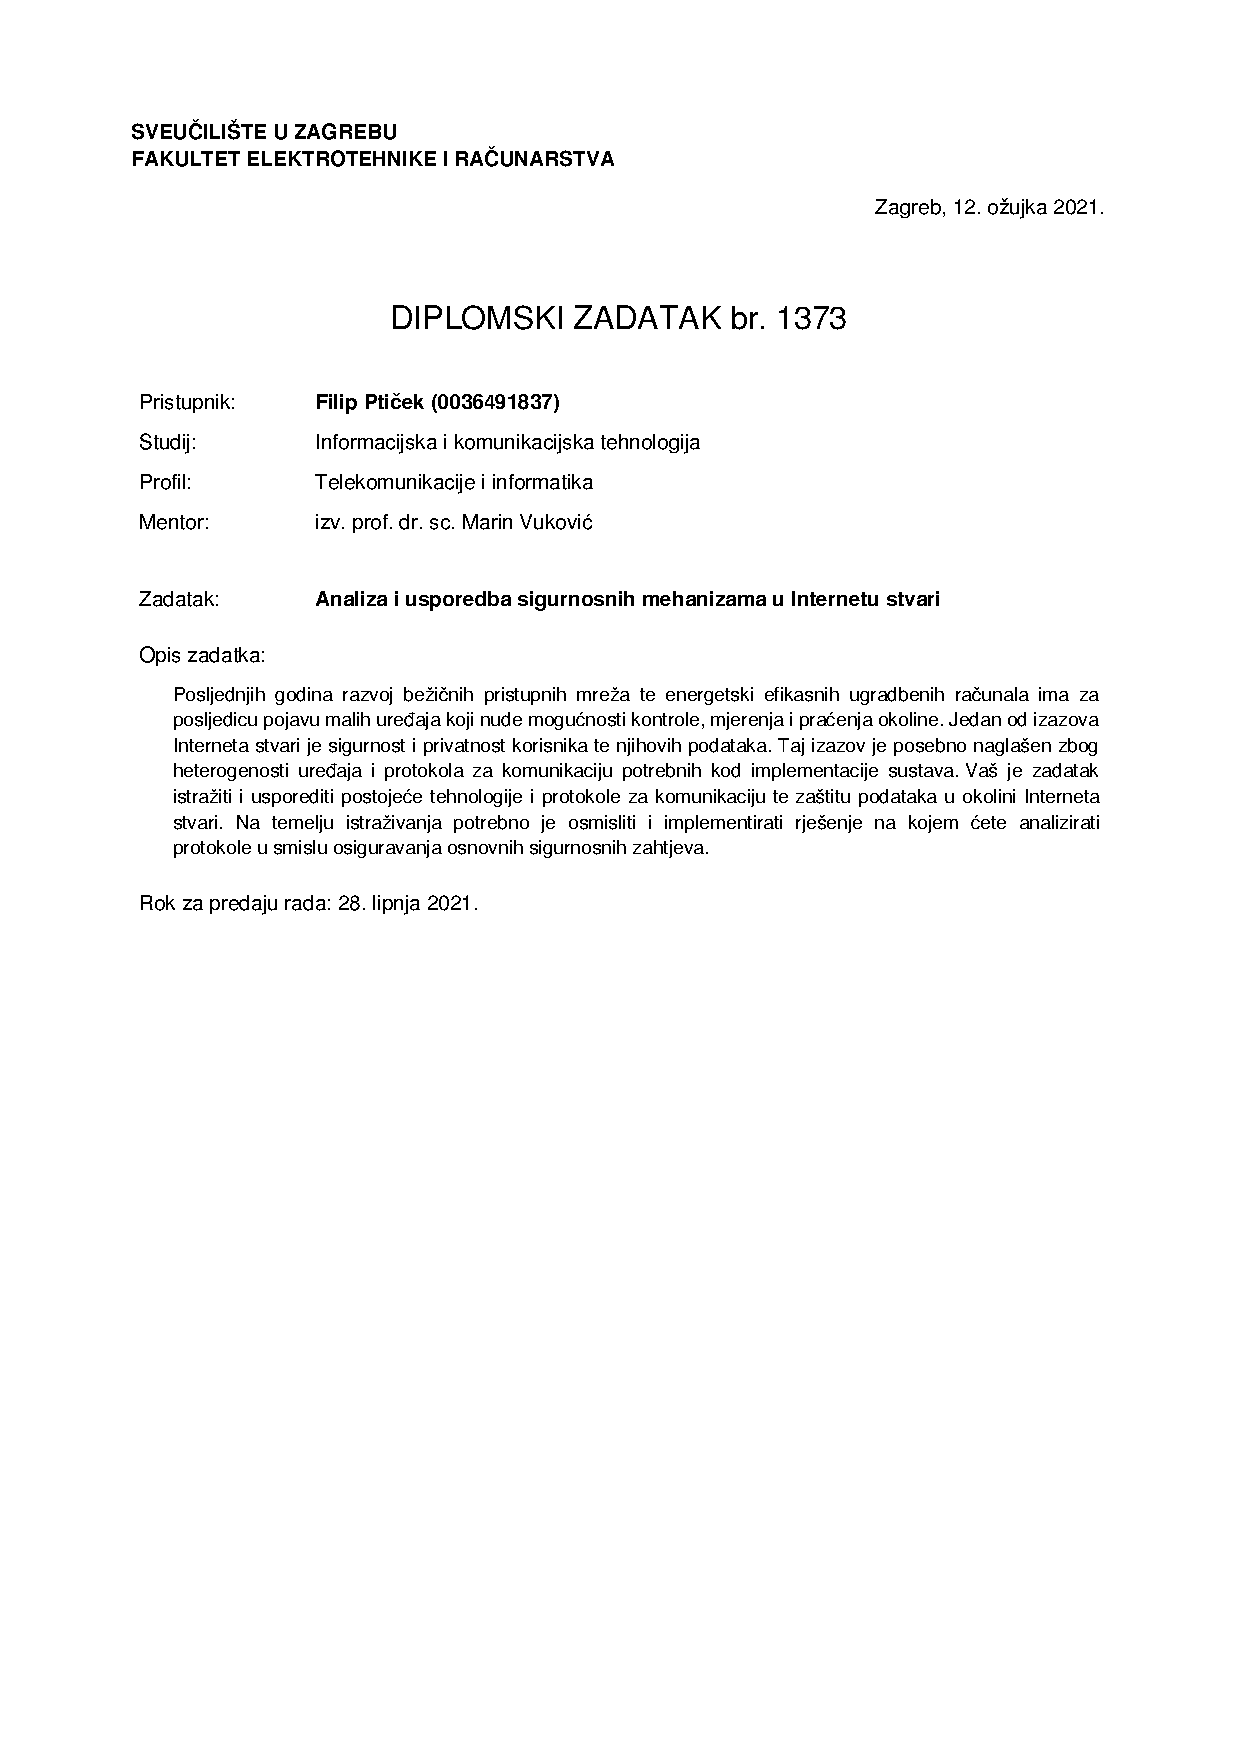
\includepdf[pages=-,fitpaper=true]{zadatak.pdf}

% Dodavanje zahvale ili prazne stranice. Ako ne želite dodati zahvalu, naredbu ostavite radi prazne stranice.
\zahvala{}

\tableofcontents

\chapter{Uvod}
Internet stvari sve više obuhvaća našu okolinu i sadašnjicu. Pojavom brzih bežičnih pristupnih mreža te sve manjih i učinkovitijih uređaja se povezanost usadila u sve aspekte naših života. Pametni domovi, pametni gradovi i industrija 4.0 samo su neki od primjera gdje Internet stvari nalazi svoju primjenu. Povezanošću uređaja i krajnjih korisnika olakšavaju se razni dnevni procesi te se pokazuje prilika za pojavom novih koji prije nisu bili mogući. Iako se pojam Interneta stvari pojavio u zadnjih dvadeset godina, potreba za umrežavanjem uređaja datira od samih početka pojave Interneta. 

Tako se prvi pametni uređaj povezan na mrežu našao u Sveučilištu Carnegie Mellon 1982. godine. Zbog iritiranosti jednog studenta, prouzročene praznim automatom za pića, on je odlučio spojiti automat na ARPANET, preteča javna mreža Internetu, kako bi mogao doznati trenutno stanje automata\citep{Coke}. Iako taj postupak tada nije bio smatran revolucionarnom idejom, broj umreženih aparata danas ukazuje na suprotno.

Trend područja Interneta stvari je u brzom rastu te poprima sve veću primjenu u svim područjima socijalnog života i poslovnih procesa te je važno definirati i rastumačiti sigurnosne mehanizme vezane uz Internet stvari kako bi implementacijska rješenja krajnjim korisnicima pružala adekvatnu razinu sigurnosti i privatnosti.

Ovaj rad primarno obrađuje sigurnosne mehanizme u Internetu stvari uz glavni naglasak na informacijsku sigurnost, analizu i usporedbu sigurnosnih mehanizama protokola te implementaciju i sigurnosnu analizu sustava za praćenje tjelesne temperature. 

U sljedećem poglavlju će se definirati pojam, referentni model, izazovi, područja primjene i trendovi u Internetu stvari. Treće poglavlje obrađuje zahtjeve vezane uz sigurnost i privatnost te sigurnosne propuste u Internetu stvari. U četvrtom poglavlju se kroz protokolni složaj Interneta stvari analiziraju i uspoređuju protokoli svakog sloja uz naglasak na sigurnosnim mehanizmima protokola. Peto poglavlje opisuje implementaciju sustava za praćenje tjelesne temperature, arhitekturu sustava, korištene razvojne alate i uređaje, opisuje rad sustava i analizu sigurnosti sustava. Konačno u zaključku se utvrđuju implementacijski i sigurnosni izazovi oko razvoja sustava Internet stvari.

\chapter{Internet stvari}

\section{Definicija}
\emph{The International Telecommunication Union(ITU-T)} je specijalizirana agencija Ujedinjenih Naroda za informacijske i komunikacijske tehnologije. ITU-T definira Internet stvari kao globalnu infrastrukturu za informacijsko društvo, koja omogućava napredne usluge međusobnim povezivanjem (fizičkih i virtualnih) stvari na temelju postojećih i razvijajućih interoperabilnih informacijskih i komunikacijskih tehnologija. Iskorištavanjem identifikacije, prikupljanja podataka, obrade i komunikacijskih sposobnosti, Internet stvari u potpunosti upotrebljava mogućnosti povezanih stvari kako bi ponudio usluge za mnogo različitih primjena, uz osiguravanje sigurnosti i privatnosti. Sa šire perspektive, Internet stvari može biti percipiran kao vizija s tehnološkim i društvenim implikacijama\citep{ITU-T/IoT}. Informacijske i komunikacijske tehnologije (ICT) pružaju komunikaciju u bilo koje vrijeme i na bilo kojem mjestu dok Internet stvari dodaje još jednu dimenziju gdje se radi o bilo kojoj stvari u komunikaciji. Te tri dimenzije komunikacije su prikazane na sljedećoj slici.
\begin{figure}[htb]
    \centering
    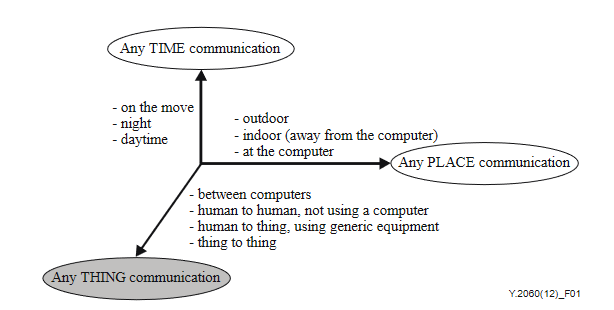
\includegraphics[width=14cm]{images/3dimenzije.png}
    \caption{Nova dimenzija komunikacije predstavljena u Internetu stvari\citep{ITU-T/IoT}}
    \label{fig:3-dim}
\end{figure}

ITU-T također definira pojmove uređaja i stvari u kontekstu Interneta stvari. Uređaj je dio opreme s obaveznom mogućnošću komunikacije i neobaveznim mogućnostima opažanja, aktuacije te prikupljanja, pohrane i obrade podataka. Pojam stvari je definiran kao objekt u fizičkom svijetu (fizička stvar) ili u informacijskom svijetu (virtualna stvar) koja ima sposobnost da bude identificiran i integrirana u komunikacijsku mrežu. Fizičke stvari postoje u fizičkom svijetu i imaju sposobnosti biti opažene, aktuirane i povezane, a virtualne stvari postoje u informacijskom svijetu i imaju sposobnosti biti spremljene, obrađene i pristupljene. Neki od primjera fizičkih stvari su: okolina, industrijski roboti, proizvodi i električna oprema, dok primjeri virtualnih stvari su multimedijski sadržaji i programska podrška.

\section{Referentni model}
Ako promatramo Internet stvari kao jedan zaseban ekosustav potrebno je definirati referentni model prema kojem možemo opisati sve dijelove sustava i njegove zahtjeve. S obzirom na to da je Internet stvari pojam koji opisuje povezanost stvari, a ne i konkretan referentni model, od pojave samog pojma su se predlagani različiti modeli koji bi predstavljali cijeli spektar mogućnosti i zahtjeva Interneta stvari. 
\begin{figure}[htb]
    \centering
    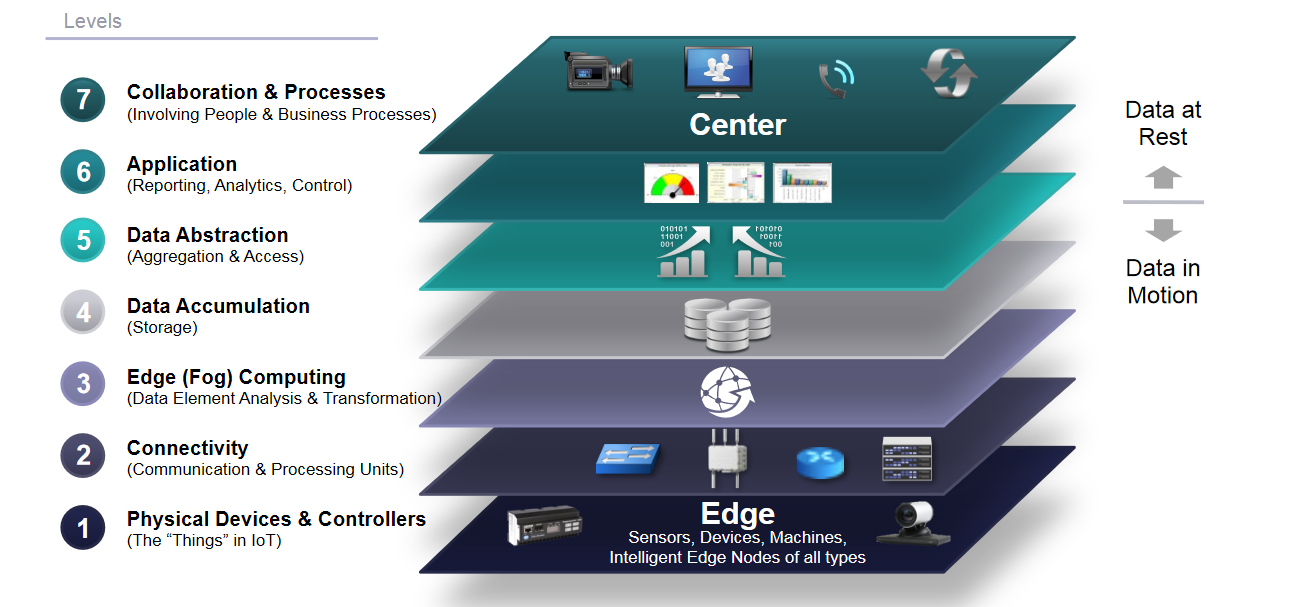
\includegraphics[width=14cm]{images/ciscomodel.png}
    \caption{Cisco Internet stvari referentni model\citep{CiscoIotModel}}
    \label{fig:ciscomodel}
\end{figure}

Ciscov referentni model Interneta stvari\citep{CiscoIotModel} definira višeslojni model od kojih svaki sloj definira terminologiju koja može biti standardizirana kako bi se stvorio globalni referentni okvir. Ovaj model ne definira lokalnost komponenata već opisuje zadatke koje svaki sloj obavlja kako bi se održala jednostavnost, omogućila skalabilnost i osigurala potpora. Model također definira funkcije koje su potrebne kako bi sustav Interneta stvari bio kompletan. Na slici 2.2 je prikazan Ciscov Internet stvari referentni model i njegovi slojevi. Put podataka između slojeva je dvosmjeran, dok put kontrolnih informacija je s viših slojeva prema nižim slojevima. Kod promatranja je put informacija u obrnutom smjeru, od nižih slojeva prema višim. 

\subsection{Fizički uređaji i kontroleri}
Referentni model počinje s prvim slojem: fizički uređaji i kontroleri koji mogu upravljati s više uređaja. Ovo je sloj koji opisuje stvari u kontekstu Interneta stvari i uključuje različiti raspon uređaja koji šalju i primaju informacije. Uređaji 
su različitih veličina, izgleda i namjene te potječu od različitih proizvođača. Kako bi se pojednostavila kompatibilnost referentni model općenito opisuje razinu obrade potrebne od uređaja. Neke od osnovnih sposobnosti uređaja uključuje: pretvorbu analognih u digitalne signale, generiranje podataka i mogućnost da se uređajem upravlja i šalju upiti.

\subsection{Povezanost}
Komunikacije i povezanost su sadržani u drugom sloju. Najvažnija mogućnost ovog sloja je sposobnost pouzdanog i pravovremenog prijenosa informacija. Time se definira prijenos između uređaja i mreže, između mreža te između mreže i računanja na rubu mreže \engl{Edge Computing} na trećem sloju. Jedan od cilja referentnog modela je da se sva komunikacija odvija putem postojećih mreža. Kako neki uređaji ne podržavaju protokol IP, potrebno je u mrežu uvesti prilaze \engl{gateway} koji će služiti kao posrednik između uređaja i ostatka mreže. Na ovom sloju se pojavljuje velika heterogenost komunikacijskih i pristupnih protokola koji uvelike ovise o željenoj namjeni uređaja prvog sloja. Ovaj sloj je usko povezan sa TCP/IP složajnim modelom koji sadrži protokole fizičkog sloja, sloja podatkovne poveznice te mrežnog, transportnog i aplikacijskog sloja.

\subsection{Računarstvo na rubu mreže}
Funkcija trećeg sloja je vođena potrebom za pretvaranjem mrežnog podatkovnog prometa u informacije koje su prikladne za pohranu podataka i za obradu na višim slojevima. Treći sloj je zadužen za obradu podataka i njihovu transformaciju. Jedno od načela ovog referentnog sloja je da se obrada podataka odvija što je ranije moguće i što bliže rubu mreže kako bi se smanjila potreba za odvijanjem obrade velikog skupa podataka na udaljenom i centralnom mjestu. Obrada na trećem sloju obuhvaća razne primjere poput: evaluacije, formatiranja, proširivanja, dekodiranja, redukcije i procjene značenja podataka.

\subsection{Akumulacija podataka}
Mrežni sustavi su izgrađeni za pouzdani prijenos podataka. Prije četvrtog sloja podaci su u stanju prijenosa. Takvi podaci proizlaze iz prvog i prolaze kroz drugi i treći sloj. Kako u nekim slučajevima ne postoji potreba za trenutnom obradom tih podataka, oni dolaze do četvrtog sloja gdje se podaci spremaju u memoriju. Na ovom sloju su podaci trajni i nepromjenjivi te spremni za posluživanje višim slojevima referentnog modela. Četvrti sloj određuje jesu li podaci važni za više slojeve, ako jesu, potrebno je osigurati načine posluživanja tih podataka zahtjevima viših slojeva. Određuje je li potrebno da podaci budu trajni, tj. treba li podatke spremiti na trajnu ili ih je dovoljno spremiti u radnu memoriju za kratkoročnu upotrebu. Kakav tip pohrane podataka je potreban: datotečni sustav, distribuirani datotečni sustav ili neki oblik baze podataka. Na koji način je organizirano spremanje podataka te je li potrebno podatke spojiti, preračunati i agregirati s prethodno spremljenim podacima. Ukratko, zadaća četvrtog sloja je da podatke bazirane na događajima pretvori u podatke nad kojima se rade upiti za potrebe viših slojeva.

\subsection{Apstrakcija podataka}
Funkcije apstrakcije podataka petog sloja su fokusirane na prikazivanje podataka i njihovu pohranu na način koji dozvoljava razvoj jednostavnijih, brzih aplikacija. Kako u modelu Interneta stvari postoji više uređaja koji generiraju podatke tako postoje različiti razlozi zašto podaci nisu prisutni na istom podatkovnom spremištu: previše podataka za spremanje na jedno mjesto, uređaji su geografski odvojeni, a obrada je optimizirana lokalno, postoji potreba za različitim načinima obrade podataka te se koriste različiti načini akumulacije podataka. Zbog tih razloga peti sloj je zadužen za različite vrste obrade poput ujednačavanja različitih formata podataka iz različitih izvora, osiguravajući dosljednu semantiku podataka kroz različite izvore, potvrda o potpunosti podataka šestom aplikacijskom sloju, zaštita podataka korištenjem autorizacijskih i autentifikacijskih mehanizama te normaliziranje i indeksiranje podataka za brz pristup od strane aplikacija.

\subsection{Aplikacije}
Na šestom sloju se nalazi aplikacijski sloj koji obavlja interpretaciju informacija. Ovaj referentni model ne definira strogo aplikaciju. Aplikacije se razlikuju na temelju različitih tržišta, prirode podataka i poslovnih potreba. Primjeri različitih potreba su aplikacije koje su usredotočene na promatranje i prikupljanje podataka, neke aplikacije se koriste za kontrolu uređaja dok neke kombiniraju podatke s uređaja i drugih izvora. Aplikacije predstavljaju različite modele upotrebe, razvojnih obrazaca, korištene razvojne programske podrške te krajnje kompleksnosti upotrebe. Neki primjeri aplikacija su povezane sa specijaliziranim industrijskim rješenjima, mobilne aplikacije koje obavljaju jednostavne interakcije, izrada izvješća povezanih uz poslovne procese, analitičke aplikacije koje obrađuju i interpretiraju podatke važne za poslovne odluke i aplikacije za upravljanje i kontroliranje ostatkom sustava. Ako su prijašnji slojevi dizajnirani pravilno to će utjecati na količinu posla koje sama aplikacija mora raditi dok će to zauzvrat olakšati procese na sedmom sloju. 

\subsection{Suradnja i procesi}
Zadnji sedmi sloj referentnog modela uključuje ljude i poslovne procese. Ljudi koriste aplikacije i pridružene podatke za svoje specifične potrebe. Često, više ljudi koriste iste aplikacije za različite svrhe. Tako cilj cijelog sustava Interneta stvari nije sama aplikacija nego kao ispomoć u radu ljudi. Aplikacije pomažu ljudima kako bi mogli obavljati različite poslovne procese uz odgovarajuće podatke u pravo vrijeme. Poslovni procesi nerijetko uključuju rad i komunikaciju između više ljudi. Ljudi surađuju i komuniciraju međusobno kako bi potpora Interneta stvari bila korisna. Zato ti procesi zahtijevaju više koraka koji obuhvaća više aplikacija. Stoga zadnji sloj predstavlja višu razinu od jedne aplikacije.

\section{Izazovi}
Internet stvari kao pojam i skup tehnologija donosi i određene izazove. S obzirom na to da je Internet stvari široko područje, koje ima različita područja primjene, tako su i izazovi s kojima se susreće kod razvoja, planiranja i održavanja sustava brojni. Korištenjem pravilnih oblikovnih obrazaca postižu se bolja svojstva sustava te se olakšava daljnje održavanje i korištenje. U nastavku su nabrojani i opisani neki od izazova koji se pojavljuju u sustavima Interneta stvari.

\subsection{Heterogenost}
Heterogenost se pojavljuje na svakom implementacijskom koraku Internet stvari sustava. Heterogenost uređaja, komunikacijskih, pristupnih i transportnih protokola, programske podrške i samih potreba korisnika. Naravno ovakva vrsta heterogenosti se javlja zbog različitih potreba i radnih procesa. Uređaji koji se koriste nude različite potrebe u vidu veličine, potrebe za vanjskim napajanjem te dometu komunikacijskih kanala, radilo se o žičanoj ili bežičnoj komunikaciji. Protokoli koji vrše komunikaciju između uređaja i nekog oblika prilaza također ovise o tim potrebama, radilo se o potrebi za velikim transportnim brzinama ili o korištenje radiokomunikacije niske snage kako bi se očuvala energija uređaja. Također treba li komunikacija biti pouzdana i sigurna ovisi o korištenju različitih transportnih protokola te kriptografskih algoritama. Na sve navedeno utječu i sami radni procesi i potrebe korisnika. Ovisno o tome sami sustavi su osmišljeni za potrebe korisnika.

Heterogenost koja se javila u prvim razdobljima razvoja Interneta svari je povezano s nepostojanjem standardizacije i interoperabilnosti uređaja i postojećih programskih platformi. Tako se na primjeru pametnih domova pojavili različiti pametni uređaji od kojih je svaki zahtijevao vlastitu programsku platformu za upravljanje zbog nepostojanja interoperabilnosti s centralnim upravljačkim platformama. Kroz vrijeme su se pojavili zajednički napori proizvođača i različitih standardizacijskih tijela da se ovisno o području primjene Interneta stvari sustava postigne standardizacija komunikacijskih protokola i semantike informacija kako bi se postigla bolja interoperabilnost.

\subsection{Raspodijeljenost}
Kako u sustavima Interneta stvari sudjeluju različiti uređaji različitih prostornih lokacija tako se javlja i potreba za raspodijeljenosti sustava. Uređaji mogu biti mobilni što uvelike utječe na način pristupa krajnjim programskim platformama s kojima uređaji komuniciraju. Od dovođenja uređaja u sustava, upravljanja uređaja, promatranja uređaja i samih aplikacija preko kojih se ti postupci provode se odvijaju raspodijeljenim putem. U nekim sustavima broj sudionika dostiže veliku brojku te je kod takvih sustava važno da se paralelno i konkurentno mogu odvajati aktivnosti. Otpornost na kvar je još jedan od zahtjeva koji prati raspodijeljene sustave kako bi se omogućio nesmetan rad sustava. Kod ispada i kvarova posljedice koje sustav Interneta stvari može imati na vanjski svijet je velik. Posebice u primjerima gdje se nadzire neki kritični sustavi poput industrijskih postrojenja. Također u pametnim domovima gdje različiti kućanski aparati su pretvoreni u pametne uređaje, kvarom poslužitelja mogu postati neupotrebljivi te je važno da postoji redundantnost servisa s kojima uređaji komuniciraju.

\subsection{Sigurnost}
Sigurnost informacija i samih sustava je važan aspekt Interneta stvari u kojem sve više uređaja oko nas postaje umreženo. Problemi koji se javljaju su povezani s pokušajem brzog razvoja rješenja zbog konkurentnosti na tržištu, stavljanje u prvobitni plan funkcionalnosti sustava te dostupnosti prema korisnicima što stavlja sigurnost tih sustava u drugi plan. Kako mnogi uređaji i cjelokupni sustavi uvelike imaju kritične zadatke, poput medicinskih uređaja ili automobila, kompromitacija istih zbog sigurnosnih propusta može imati negativne posljedice. Također neki od primjera napada na sustave nije kako bi se napravila šteta sustavu, već za iskorištavanje procesne snage sustava u botnetovima. Sigurnosni propusti se mogu pojaviti na svakom dijelu sustava: uređaja, komunikacijskih kanala, poslužitelja, baza podataka i korisničkih sučelja. Neki od najvažnijih sigurnosnih zahtjeva na koje treba obratiti pozornost tijekom razvoja sustava Interneta stvari su obrađeni u trećem poglavlju.

\subsection{Privatnost}
Privatnost je uz sigurnost izazov s kojim se susreću mnogi sustavi Interneta stvari. Pametni uređaji koji se nalaze u našoj blizini imaju mogućnosti pratiti i bilježiti podatke o nama i našoj okolini. Kako korisnici priključuju sve više i više uređaja to je količina prikupljenih podataka veća, čime i povreda privatnosti može imati negativne posljedice na korisnika. Povrede te privatnosti mogu dolaziti u različitim oblicima. Od osobnih informacija koje mogu detaljno identificirati korisnika daju mogućnost napada u obliku krađe identiteta, medicinskih podataka ili pristupnih lozinki različitim servisima do kompromitacije sigurnosnih kamera što dozvoljava napadačima izravno praćenje korisnika. Privatnost podataka koji nisu isključivo vezani uz krajnje korisnike su i podaci pravnih osoba gdje može doći do narušavanja poslovnih tajni, autentifikacijskih i autorizacijskih podataka za razne servise i sigurnosne sustave. Kako pristupiti zaštiti privatnosti je usko povezano sa sigurnošću sustava te je obrađeno u trećem poglavlju.

\subsection{Integracija}
Nove tehnologije donose i nove integracijske probleme sa sobom. U slučaju Interneta stvari ovaj izazov je veći zbog heterogenosti svih dijelova koji čine sustave. U slučaju heterogenosti sloja podatkovne poveznice i količine različitih protokola koji se koriste postoji problem uvođenja novih prijamnika i prilaza za te uređaje. Radi li se o niskofrekventnim rješenjima poput NFC-a ili protokolima poput ZigBee postoji potreba korištenja posebnih čitača ili prijamnika dok se taj problem ne pojavljuje kod protokola Wi-Fi čija pristupna točka već postoji u većini domova. Nakon toga dolazimo do komunikacijske integracije između uređaja i poslužitelja, tj. programskih platformi. Na koji način će se odvijati prijenos podatka, kako će ti podaci biti organizirani te semantičko značenje tih istih podataka. Početkom razvoja rješenja Interneta stvari prvobitno su svi sustavi imali vlastite pristupne aplikacije. S pojavom želje za automatizacijom i međusobnom komunikacijom između uređaja različitih proizvođača počele su se razvijati platforme koje omogućuju interoperabilnost među sustavima te mogućnost upravljanja i praćenja uređaja putem jedne pristupne aplikacije. Kroz razvoj tih platformi proizvođači su počeli integrirati nove i postojeće uređaje da budu kompatibilni s njima.

\section{Područja primjene}
Internet stvari je širok u svojem području primjena. U današnjem svijetu postaje sve prisutnije u svakom aspektu života ljudi i taj trend će se nastaviti. Od naših domova do industrijskih postrojenja Internetu stvari omogućava pojednostavljenje naših života i poslovnih procesa. U nastavku su navedeni neke od glavnih područja primjene Interneta stvari i rješenja koja se koriste u tim područjima:
\begin{itemize}
    \item Pametni dom
    \begin{itemize}
        \item Pametna rasvjeta
        \item Pametni kućanski aparati
        \item Detekcija uljeza
        \item Upravljanje energijom
    \end{itemize}
    \item Pametni grad
    \begin{itemize}
        \item Pametni parking
        \item Upravljanje otpadom
        \item Pametna rasvjeta
        \item Reagiranje na hitne slučajeve
    \end{itemize}
    \item Okoliš
    \begin{itemize}
        \item Praćenje vremena
        \item Praćenje zagađenja zraka
        \item Praćenje zagađenja bukom
        \item Detekcija požara
    \end{itemize}
    \item Prodaja
    \begin{itemize}
        \item Upravljanje inventarom
        \item Pametni automati za prodaju
        \item Pametne blagajne
        \item Pametno plaćanje
    \end{itemize}
    \item Logistika
    \begin{itemize}
        \item Praćenje flote vozila
        \item Praćenje pošiljaka
        \item Dijagnostika vozila na daljinu
        \item Generiranje i vremensko raspoređivanje voznih ruta
    \end{itemize}
    \item Industrija
    \begin{itemize}
        \item Dijagnostika strojeva
        \item Praćenje dijelova proizvodnje
        \item Automatizacija proizvodnih procesa
    \end{itemize}
    \item Poljoprivreda
    \begin{itemize}
        \item Pametno navodnjavanje
        \item Praćenje usjeva
        \item Automatizacija obrađivanja
    \end{itemize}
\end{itemize}

\section{Trendovi}
Internet svari se pojavio kao zamisao za daljnju budućnost, ali je već danas sadašnjost u socijalnim i proizvođačkim aspektima svijeta. To može biti pripisano pristupačnijim, procesorski bržim, energetski učinkovitijim te sve manjim uređajima za kojima raste potražnja integracije takvih rješenja u različita područja koja također kroz vrijeme postaju sve raznovrsnija. Trenutni broj umreženih Internet stvari uređaja doseže brojku od 35.82 bilijuna uređaja. Pojavom novih tehnologija poput 5G mreža, koje dozvoljavaju još veće brzine i smanjeno vrijeme odaziva, taj trend će kroz godine još više rasti te su neke od projekcija za godinu 2025. u iznosu od 75.44 bilijuna uređaja\citep{IotNumber}. Trend broja umreženih Internet stvari uređaja između 2015. godine i predikcije do 2025. godine su prikazane na sljedećoj slici. 
\begin{figure}[H]
    \centering
    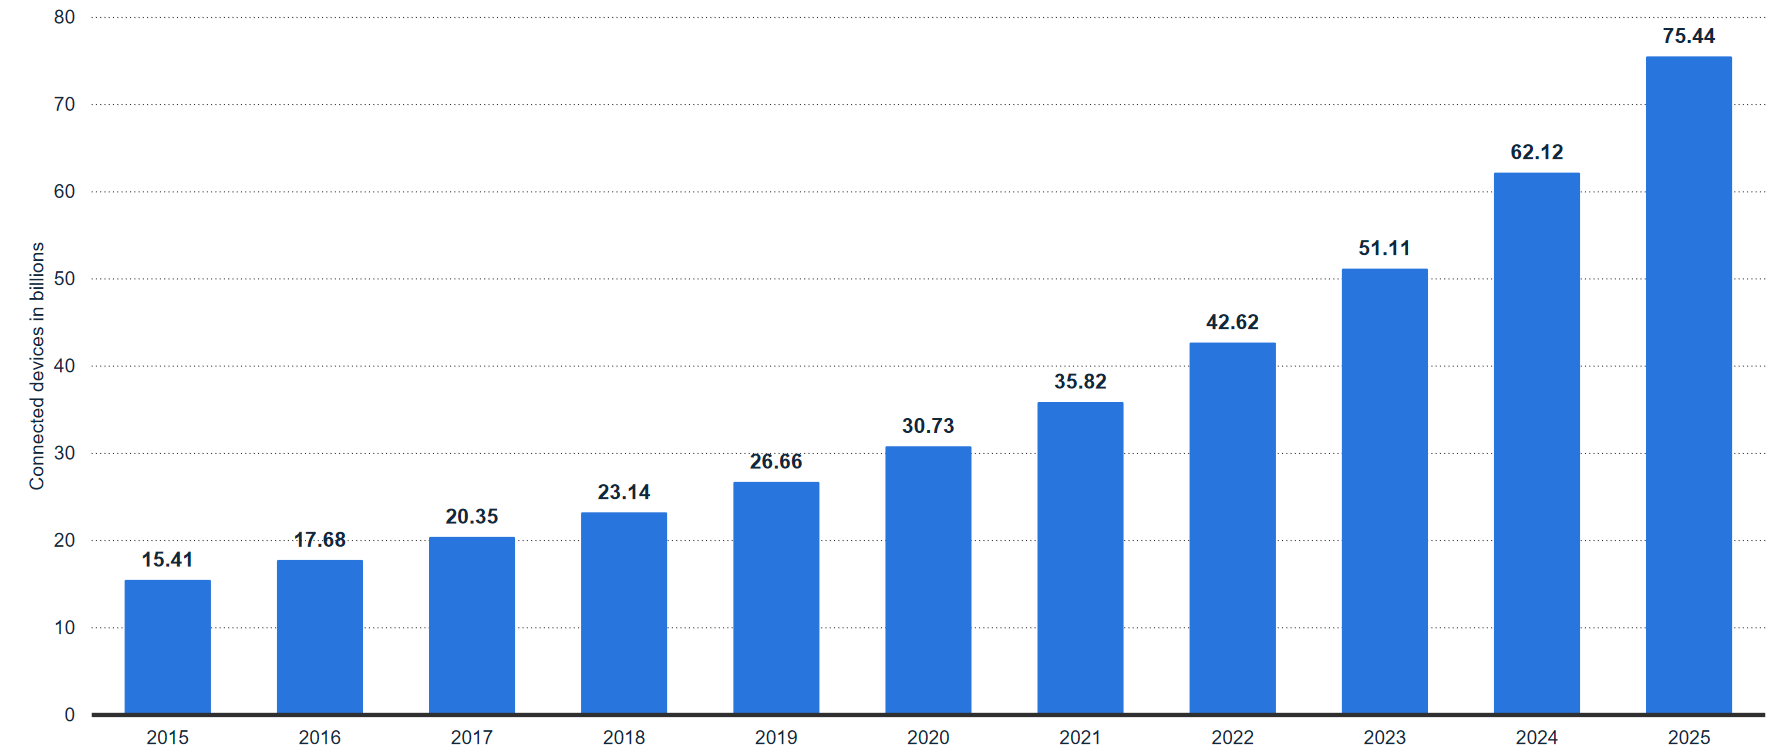
\includegraphics[width=14cm]{images/number-of-installed-iot.png}
    \caption{Broj povezanih Internet stvari uređaja\citep{IotNumber}}
    \label{fig:iotdevices}
\end{figure}

Ako promatramo porast broja umreženih Internet stvari uređaj možemo zaključiti da s time postoji i veliki tržišni potencijal. Korisnika je sve više te je procijenjeno da svaki posjeduje prosječno četiri Internet stvari uređaja te da se u svijetu svake sekunde spoji novih 127 uređaja. Tako su i procjene za ekonomski utjecaj Interneta stvari na tržište između 3.9 i 11.1 bilijuna američkih dolar kroz različita područja primjene uključujući tvornice, gradove, domove i prodaju\citep{Patel2018Jan}. Na sljedećoj slici su prikazane niske i visoke predikcije za ekonomski utjecaj Interneta stvari za 2025. godinu.
\begin{figure}[H]
    \centering
    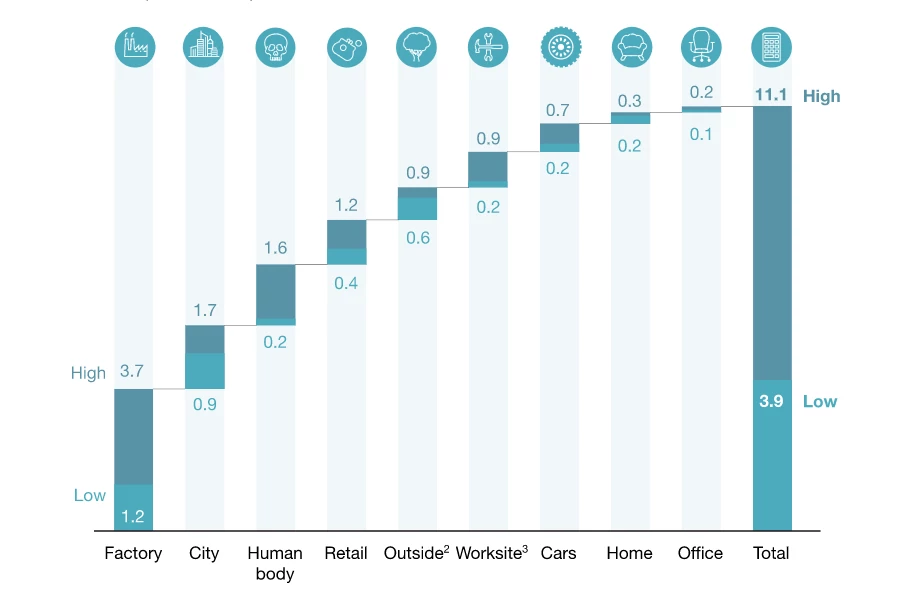
\includegraphics[width=12cm]{images/iot-economic-impact.png}
    \caption{Potencijalni ekonomski utjecaj Interneta stvari kroz različita područja primjene za 2025. godinu. izražen u bilijunima američkih dolara\citep{Patel2018Jan}}
    \label{fig:market}
\end{figure}

\chapter{Sigurnost u Internetu stvari}
\section{Zahtjevi vezani uz sigurnost i privatnost}
Važnost sigurnosti i privatnosti je nezamjenjiva. Ta važnost se posebice očituje u sustavima Interneta stvari gdje je ponekad veći naglasak stavljen na funkcionalnost što stavlja sigurnosne zahtjeve u drugi plan. Jednostavni uređaji s malo procesorske snage imaju problema s obavljanjem zahtjevnijih kriptografskih algoritama te je studija iz 2019. godine utvrdila da od 56 milijuna ispitanih uređaja, 91.5\% razmjene podataka je bilo nešifrirano\citep{Greene2019May}. Nedostatak iskustva u području razvoja Interneta stvari također utječe na slabu sigurnost uređaja jer se ponekad kod planiranja ne utvrde svi mogući sigurnosni propusti te zahtjevi koji su vezani uz sigurnost i privatnost. Ti zahtjevi su ključan dio očuvanja sigurnosti cjelokupnog sustava i privatnosti samih korisnika. Zahtjevi vezani uz sigurnost i privatnost su sljedeći\citep{InternetStvari}:

\begin{description}
    \item[Tajnost:]informacija nije dostupna ili je izložena  neovlaštenim osobama, entitetima ili procesima.
    \item[Cjelovitost:]točnost i potpunost informacije.
    \item[Raspoloživost:]informacija je dostupna na zahtjev i omogućeno je njeno korištenje od strane ovlaštenih osoba, entiteta ili procesa.
    \item[Vjerodostojnost:]osoba, entitet ili proces je zaista onaj kojim se predstavlja.
    \item[Odgovornost:]obveza izvještavanja o aktivnostima i preuzimanja odgovornosti za njih.
    \item[Neporicanje:]sposobnost dokazivanja događaja ili aktivnosti i osoba, entiteta ili procesa koji su ih pokrenuli ili u njima sudjelovali.
    \item[Pouzdanost:]konzistentno ponašanje i rezultati.
\end{description}

\section{Sigurnosni propusti}
The Open Web Application Security Project® (OWASP) je neprofitna organizacija čiji je cilj napredak i poboljšanje računalne sigurnosti informacijskih sustava. OWASP kroz svoje projekte otvorenog koda vođenih putem razvojne zajednice radi na poboljšanju sigurnosti Interneta.

\emph{OWASP Internet of Things Project} je projekt osmišljen kako bi pomogao proizvođačima, programerima i potrošačima bolji uvid i razumijevanje u sigurnosne probleme vezane uz Internet stvari. Tako korisnici u bilo kojem dijelu razvojnog procesa mogu donositi bolje odluke kod razvoja, postavljanja i pristupanja tehnologijama Interneta stvari\citep{owasp1}. 2018. godine izlazi \emph{OWASP IoT Top 10} lista koja reprezentira deset najčešćih ranjivosti Internet stvari sustava. Svih deset sigurnosnih ranjivosti su navedeni u nastavku uz opis sigurnosnih praksi koje bi trebale spriječiti te ranjivosti i sigurnosne propuste. 

\subsection{Slabe, pogodljive ili tvrdo kodirane lozinke}
Prvi navedeni sigurnosni problemi kod Internet stvari sustava su vezni uz lozinke. Da bi se uređaju moglo pristupiti i naknadno ga konfigurirati, uređaji dolaze s korisničkim računima koji služe korisnicima kako bi ih mogli upariti sa željenim sustavom ili kako bi proizvođač mogao upravljati uređajem u slučaju pomoći korisnicima ili kod ažuriranja uređaja. Za pristup tom korisničkom računu uređaja je potrebna lozinka koju krajnji korisnik kod prve upotrebe treba postaviti. Navike korisnika su većinom da iskoriste njima dobro poznatu lozinku koju koriste i za svoje druge korisničke račune. Ako napadač dobije pristup jednoj njihovoj lozinki ima i pristup ostalim računima. Na taj način se pristup korištenim uređajima koji imaju isto korisničko ime ili e-mail adresu i lozinku uvelike olakšava. Korisnici imaju i naviku koristiti slabe lozinke koje su vrlo česte i jako lako pamtljive. Tako su neke od najčešće korištenih lozinka jednostavni nizovi numeričkih znakova ili nizovi znakova na tipkovnici poput: 123456, 123456789, qwerty, ili sam engleski prijevod lozinke \engl{password}\citep{pass1}. Napadi na lozinke se provode putem takozvanih \emph{brute force} napada. Kako je procesna snaga današnjih računala dosegla vrlo visoke brzine računanja, tako se jednostavne i kratke lozinke mogu pogoditi u vrlo kratkom vremenu.

Ovakvi propusti ne zaobilaze ni proizvođače samih sustava i uređaja. Kod proizvodnje proizvođači na uređaje postavljaju iste lozinke za sve uređaje kako bi kod testiranja ispravnosti lakše pristupili istima. Jedan od najboljih pokazatelja takvog pristupa su usmjerivači/modemi telekom operatera za pristup Internetu koji imaju postavljenu istu zadanu lozinku i korisničko ime poput "admin" ili "user" koju krajnji korisnici uređaja nikada ne promjene. Problem se također pojavljuje i u tvrdo kodiranim \engl{hard coded} lozinkama. Proizvođači postave takve lozinke na uređaje kako bi se uređaji mogli nesmetano povezati s vanjskim servisima, kako bi se proizvođači povezali na uređaj zbog otklanjanja pogrešaka ili kao način za vanjsko upravljanje uređajima. Ako napadač ima fizički pristup uređaju on može skenirati memoriju i pomoću raznih alata pronaći lozinku spremljenu na samom uređaju. A kako proizvođači najvjerojatnije koriste istu lozinku za sve iste modele uređaja, napadač ima lak način za pristup i ostalim istim uređajima.

Kako bi se spriječila ova vrsta ranjivosti neki od sigurnosnih mjera koji bi se trebali pratiti su sljedeći. Korisnici bi kod prve upotrebe uređaja trebali promijeniti zadanu lozinku koristeći duge, kompleksne i jedinstvene nizove znakova. Najjednostavniji način za postići te zahtjeve je korištenjem upravitelja lozinkama. Oni daju mogućnost generiranja lozinki uz mogućnost spremanja istih bez potrebe da korisnik mora pamtiti sve jedinstvene i duge lozinke. Što se tiče zahtjeva od strane proizvođača, oni bi trebali razriješiti bolje načine upravljanja uređajima kako bi se izbjeglo korištenje istih ili čak tvrdo kodiranih lozinka za pristup uređaju ili vanjskim servisima. Također bi proizvođači trebali upozoriti korisnika kod uspostave uređaja da promijeni zadanu lozinku.

\subsection{Nesigurne mrežne usluge}
Internet stvari uređaji koriste razne mrežne usluge kako bi mogli komunicirati s vanjskim servisima. Kako je moguće pristupiti tim uređajima putem Interneta potrebno je pravilno osigurati sigurnost tih mrežnih usluga koje se izvršavaju. Neautoriziran pristup preko usluga iskorištavajući zadane lozinke, otvorene mrežne priključke te nepravilno podešeni vatrozidi dozvoljavaju napadaču da dobije pristup uređajima i poslužiteljima. Takvi napadi dozvoljavaju izvršavanje malicioznog koda, iskorištavanje uređaja za botnet, krađu podataka ili onesposobljavanje sustava.

Neki od sigurnosnih mjera koje se mogu poduzeti za osiguravanje mrežnih usluga su: \begin{itemize}
    \item korištenje zasebne lokalne mreže za sve pametne uređaje,
    \item spajati uređaje na isključivo sigurne mreže,
    \item instaliranje regularnih softverskih ažuriranja,
    \item isključivanje svih usluga koje pružaju vanjski pristup uređaju,
    \item isključivanje nepotrebnih mrežnih priključaka i usluga,
    \item isključivo korištenje protokola koji podržavaju šifriranje.
\end{itemize}

\subsection{Nesigurna sučelja ekosustava}
Nesigurna web sučelja, pozadinski API-jevi, servisi u oblaku i mobilna sučelja, koja dozvoljavaju komunikaciju i interakciju s uređajem, čine sveukupni ekosustav Interneta stvari. Kompromitacija bilo kojeg dijela sustava može uzrokovati i kompromitaciju cjelokupnog sustava. Ranjivost kod načina autorizacije i autentifikacije između uređaja i poslužitelja ili korisnika mobilnih i web aplikacija i poslužitelja su jedan od vektora napada na sustav. Također nedostatak ili korištenje slabog šifriranja kod komunikacije može uzrokovati da napadač presretne i iskoristi sakupljene informacije za napad. Nedostatak pravilnog filtriranja ulazno/izlaznih podataka može dovesti do napada poput SQL injekcije. Još jedan projekt OWASP organizacije je \emph{OWASP Top 10 Web Application Security Risks} koji nudi popis najčešćih ranjivosti za web i mobilne aplikacije. Nesigurna sučelja ekosustava imaju direktnu poveznicu s tim ranjivostima koje su: \begin{itemize}
    \item injekcije (SQL, NoSQL, OS, LDAP),
    \item neispravna autentifikacija,
    \item izlaganje osjetljivih podataka,
    \item XML External Entities(XXE) napadi,
    \item neispravna autorizacijska kontrola,
    \item pogrešna konfiguracija servisa,
    \item Cross-Site Scripting(XSS),
    \item nesigurna deserijalizacija podataka,
    \item korištenje biblioteka i komponenta s poznatim sigurnosnim ranjivostima,
    \item nedovoljno korištenje logova i praćenja sustava.\citep{owasp2}
\end{itemize}

Pravilno podešavanje autorizacije i autentifikacije korisnika, ali i uređaja je najvažniji način osiguravanja raznih sučelja ekosustava. Filtriranje ulaznih i izlaznih podataka spriječava napade injekcijom, pravilno podešavanje poslužitelja da koriste kriptografske algoritme za sve servise kako bi osigurali privatnu i sigurnu komunikaciju. Kroz cijeli ekosustav je potrebna i uspostava logiranja i praćenja sustava kako bi se na vrijeme otkrila nepravilna ponašanja unutar samog sustava.

\subsection{Nedostatak mehanizama za sigurnosna ažuriranja}
Kroz vrijeme, za programska rješenja koja se trenutno koriste na uređaju će se pronaći ranjivosti. Kako bi se na vrijeme i jednostavnim putem mogli spriječiti napadi koji iskorištavaju te ranjivosti potrebna su nam softverska ažuriranja, kao i ažuriranja samog ugrađenog programa \engl{firmware} uređaja. Ako ne postoji način kojim dovodimo takva sigurnosna ažuriranja na uređaj postoji rizik za kompromitacijom uređaja. Također ako su i implementirani načini sigurnosnih ažuriranja, potrebno je pridodati pažnju na način te implementacije ažuriranja. Ako se ne provjeravaju digitalni potpisi izvora ažuriranja, moguće je na uređaj poslati maliciozno ažuriranje koje će kompromitirati uređaj. Potrebno je i koristiti sigurne načine prijenosa tih ažuriranja poput šifriranja upotrebljavanog komunikacijskog kanala. 

Trenutnim trendom brzog razvoja novih uređaja, proizvođači često ne daju dovoljno dugi period sigurnosnih ažuriranja. Tako će se desiti da proizvod nakon manje od dvije godine prestane dobivati ažuriranja te će pasti odluka na korisnika o tome hoće li kupiti novi uređaj ili riskirati kompromitaciju trenutnog. Najbolji pokazatelj toga su pametni telefoni od kojih većina tijekom svog perioda upotrebe dobije samo nekoliko sigurnosnih ažuriranja prije nego bude zapostavljena od strane proizvođača.

Kako bi se uređaji zaštili od budućih napada zbog novootkrivenih sigrunosnih propusta potrebno je pružati korisnicima uređaja nuditi dugotrajna i česta sigurnosna ažuriranja. Prijenos ažuriranja je neophodno prenositi putem sigurnih komunikacijskih kanal koji su šifrirani. Ažuriranjima koja su dostigla na uređaj je potrebno validirati izvor, provjeriti odgovara li digitalni potpis izvoru od kojeg bi trebalo stići ažuriranje te je potrebno i validirati samo ažuriranje kako bi se izbjeglo moguće umetanje malicioznog koda.

\subsection{Upotreba nesigurnih ili zastarjelih komponenti}
Nadovezano na nedostatak mehanizama za sigurnosno ažuriranje, peta po redu od sigurnosnih propusta je upotreba nesigurnih ili zastarjelih komponenti. Mnogi sustavi Interneta stvari kao dio svojeg programskog rješenja sadrže otvoreni kod koji održava zajednica koja nije direktno povezana s proizvođačem. Kada se otkrije ranjivost na nekom od korištenih otvorenih rješenja proizvođač ili čeka na sigurnosnu zakrpu, ili u najboljem slučaju će sam riješiti sigurnosni propust te ga objaviti kako bi doprinio razvoju otvorenog rješenja. Nakon što sigurnosna zakrpa bude razvijena potrebno je ažurirati sve uređaje ili dijelove sustava koji su ugroženi od tog sigurnosnog propust. 

Ako govorimo o Internetu stvari u proizvođačkoj industriji, takozvanoj Industriji 4.0, upotreba zastarjele programske podrške, koja je potrebna zbog jako specifičnih uređaja za proizvodnju, čija zadnja verzija zna datirati i više od deset godina nije rijetka. Uvođenjem takvih uređaja u sustave Interneta stvari također utječe na sigurnost i integritet cjelokupnog sustava te ugrožavanje jednog uređaja može dovesti do napada na cijelog lanca opskrbe. Kod upotrebe gotovih proizvoda poput senzora, videokamera ili pametne rasvjete te integracijom istih u postojeći sustav također treba obratiti pozornost na dostupnost sigurnosnih ažuriranja te stanja uređaja kojeg proizvođač još uvijek nudi sigurnosnu podršku.

Kod planiranja razvoja Interneta stvari sustava potrebno je uzeti u obzir trenutno, a i buduće stanje razvojne i sigurnosne podrške vanjske programske potpore i komponenti sustava. Najbolji način za sprječavanje sigurnosnih propusta je korištenje vlastito razvijene programske potpore ili korištenje dobro podržanih vanjskih biblioteka otvorenog koda s jakom i aktivnom razvojnom zajednicom. Upotreba zastarjelih uređaja bez sigurnosne podrške proizvođača ili potporom koja uskoro dostiže krajnji period \engl{end of life} je potrebno izbjegavati. Nakon puštanja sustava u produkciju nadziranje i praćenje vijesti vezanih uz sigurnosne propuste upotrebljenih komponenti i programske podrške je važno kako bi se na vrijeme moglo spriječiti kompromitacija sustava. Sve ovo nije moguće ako bilo koji dio ustava nema implementirane mehanizme za sigurnosna ažuriranja. Ako neka od komponenti dostigne svoj krajnji period ažuriranja potrebno je tu komponentu ukloniti i zamijeniti ju drugom čija sigurnosna ažuriranja još uvijek su podržana.  

\subsection{Nedovoljna zaštita privatnosti}
Uloga Interneta stvari je djelom prikupljanje različitih podataka i mjerenja. Neki od tih podataka su osobne prirode za korisnika poput: medicinskih podataka ili zvukovnih i video zapisa. Kompromitacija takvih privatnih podataka može negativno utjecati na sigurnost korisnika. Prostor na kojem se privatnost korisnika može narušiti je od samog uređaja koji prikuplja podatke, do komunikacijskih kanala preko kojih se podaci šalju do samih krajnjih servisa koji primaju i obrađuju te podatke, a zatim ih spremaju u baze podataka na poslužiteljima. Nedovoljna zaštita privatnosti je zapravo rezultat svih ostalih nabrojanih sigurnosnih ranjivosti nabrojanih u ovom odjeljku. 

Za očuvanje privatnosti korisnika i načine obrade podataka korisnika u Europskoj uniji postoji uredba donesena od strane Europske unije pod nazivom \emph{Opća uredba o zaštiti podataka(GDPR) (EU) 2016/679}\citep{GDPR}. Cilj uredbe je omogućiti građanima Europske unije veću kontrolu i uvid u podatke koji se prikupljaju. Tako građani mogu tražiti brisanje svojih podataka i povećava se odgovornost pravnih osoba koje te podatke prikupljaju. Odgovornost se postiže mogućim nametnutim sankcijama, ako se utvrdi povreda podataka građana. Prikupljanje podataka je moguće uz izrazitu privolu građana korisnika čime se zabranjuje bilo kakvo prikupljanje podataka bez pristanka. 

Šifriranje komunikacijskih kanal nekada ne osigurava i privatnost korisnika. Kako bi pametni uređaji mogli komunicirati s krajnjim poslužiteljima, koji mogu mijenjati svoju odredišnu adresu, koriste se domenska imena. Za razlučivanje tih adresa u brojčane IP adrese koristi se protokol DNS\engl{Domain Name System}. Kada uređaji rade DNS upite u sadržaju upita se prikazuje i domena upita u nešifriranom formatu. Na taj način napadač može iz konteksta upita zaključiti koji uređaji proizvođača se nalaze u mreži korisnika. Za neke uređaje je moguće zaključiti i sam tip, a ne samo proizvođača. U sljedećoj tablici možemo vidjeti uređaje i DNS upite koje proizvode:

\begin{table}[h]
    \centering
    \caption{Primjer DNS upita napravljenih od strane uređaja \citep{Apthorpe2017May}}
    \begin{tabular}{| c | c |} 
    \hline
    \textbf{Uređaj} & \textbf{DNS upiti} \\
    \hline\hline
    Nest Security Camera & nexus.dropcam.com \\
     & oculus519-vir.dropcam.com \\
     & pool.ntp.org \\
    \hline
    Amazon Echo & ash2-accesspoint-a92.ap.spotify.com \\ 
     & audio-ec.spotify.com \\ 
     & device-metrics-us.amazon.com \\ 
     & ntp.amazon.com \\ 
     & pindorama.amazon.com \\ 
     & softwareupdates.amazon.com \\
    \hline
    \end{tabular}
    \label{tab:confusion}
\end{table} 

Još jedan način na koji se može zaključiti o trenutnoj aktivnosti korisnika u vlastitoj mreži je i broj paketa koji se šalje u danom trenutku van mreže i njihova periodičnost. Ako se radi o uređaju koji ima mogućnosti virtualnog asistenta moguće je imati uvid u to kada je korisnik imao interakciju s uređajem. Također kod uređaja koji prate spavanje korisnika se broj razmijenjenih paketa drastično poveća kada korisnik spava\citep{Apthorpe2017May}.

Kako najbolje očuvati privatnost korisnika je pitanje s kojim još uvijek mnogi proizvođači imaju problema. To se očituje u ostalim navedenim sigurnosnim propustima u ovom odjeljku. Zakonskim regulativama postiže se veća svijest o bitnosti zaštite podataka te se samim time proizvođači tjeraju na bolje prakse za očuvanjem podataka. Neki od osnovnih načina zaštite korisničkih podataka su: 
\begin{itemize}
    \item šifriranje podataka u svakom aspektu sustava,
    \item prikupljanje samo nužnih podataka,
    \item anonimiziranje korisnika,
    \item bolja kontrola i uvid u podatke za korisnike.
\end{itemize}

\subsection{Nesigurni prijenos i pohrana podataka}
Podaci koji nisu šifrirani moguće je vrlo lako iščitati. Kriptografijom se postiže sigurnost i privatnost podataka. Kako bi se to postiglo podatke je potrebno šifrirati u svakom koraku njihova nastajanja, prijenosa, obrade i spremanja. Korištenje samih kriptografskih algoritama ne rezultira uvijek i zaštitom podataka. Neki kriptografski algoritmi koriste ključeve nedovoljne dužine i kao takve je potrebno malo vremena da se dešifriraju. Najveći sigurnosni propusti u nedavnoj povijesti povezani su direktno s neadekvatnim kriptografskim algoritmima ili općenitim nedostatkom šifriranja čime su ugroženi osobni podaci i lozinke korisnika\citep{DataBreaches}. Pozornost se treba posvetiti i kontroli pristupa podacima kako neautorizirani korisnici ne bi mogli pristupiti nedozvoljenim podacima. 

Osnovne sigurnosne mjere koje bi se trebale osigurati su: \begin{itemize}
    \item šifriranje podataka,
    \item pravilno korištenje PKI-a \engl{public key infrastructure},
    \item kontrola pristupa podacima,
    \item korištenje sigurnih protokola za prijenos podataka,
    \item provjera korištenih kriptografskih algoritama za ranjivosti,
    \item korištenje dugih kriptografskih ključeva.
\end{itemize}     

\subsection{Nedostatak mogućnosti upravljanja uređajima}
Nemogućnošću upravljanja uređajima ima posljedicu da uređaji u slučaju otkrivenih sigurnosnih propusta ne mogu biti ažurirani, da uređaje nije moguće na jednostavan način otkloniti i uvesti u ekosustav te naknadno proširivati njihove mogućnosti. Zato je jedan od najvažnijih sigurnosnih zadataka u Internet stvari ekosustavima upravljanje uređajima kroz njihov životni ciklus. Ako neautorizirani uređaji budu uvedeni u ekosustav, imat će mogućnost dobivanja pristupa ostalim komponentama ekosustava te nadgledanja mreže i presretanja prometa i informacija. 

Zbog heterogenosti trenutnih implementacijskih rješenja jedinstven način upravljanja uređaja je također jedan od problema koji se pojavljuju. Ako imamo više uređaja od kojih svaki zahtjeva svoju platformu i drugačiji način upravljanja, stvara se problem da neki uređaji koji ne zahtijevaju konstantnu pozornost ostanu zaboravljeni, nenadzirani i neažurirani. 

Potrebno je imati implementirane načine upravljanja, nadzora i ažuriranja uređaja prisutnih u sustavu. Otkrivanje i identifikacija uređaja je bitan korak u nadgledanju i zaštiti cijelog ekosustava. Heterogenost implementacijskih rješenja uređaja je još uvijek problem s kojim se integratori rješenja susreću, ali kako cijelo područje sazrijeva dolazimo do različitih platformi koje nude integraciju njih svih u jedinstveni ekosustav. Stoga je kod planiranja sustava potrebno uzeti u obzir uređaje kojim je moguće jedinstveno upravljati kako bi se izbjeglo zanemarivanje uređaja.

\subsection{Nesigurne zadane postavke}
Zadane postavke na pametnim uređajima povezane su uz nekoliko primjera. Takav propust se može očitovati kod univerzalno zadanih lozinka, tvrdo kodiranih lozinka ili zadanih postavka programske podrške uređaja. Univerzalne zadane lozinke se pojavljuju kao najjednostavniji način prvobitnom pristupu uređaju umjesto nekog drugog načina uspostave uređaja. Takav pristup se mora spriječiti navođenjem upozorenja ili obaveznim postupkom promjene lozinke kod prvobitnog postavljanja uređaja. Tvrdo kodirane lozinke za pristup uređajima je problem koji kod fizičkog ili vanjskog pristupa uređaju može lako dovesti do kompromitacije cijelog sustava te je korištenje takvih lozinka i načina pristupa potrebno izbjegavati. Zadane postavke programske podrške koje mogu dovesti do sigurnosnih propusta je dužnost proizvođača da tijekom testiranja i sigurnosne revizije uoči i onemogući sve nepotrebne i potencijalno nesigurne postavke programske podrške uređaja. To uključuje i sve metode koje su se koristile za testiranje i otklanjanje pogrešaka tijekom razvoja uređaja.

Ovaj sigurnosni propust nije isključivo vezan uz uređaje. Nesigurne zadane postavke se javljaju i na poslužiteljima te ostaloj opremi koja sudjeluje u cijelom lancu komunikacije. Usluge koje se javljaju kao zadane na operativnim sustavima poslužitelja ponekad su i nepotrebne za rad sustava. Takve usluge mogu imati zadane postavke koje dozvoljavaju jednostavan ili nesiguran pristup poslužitelju. Ovakav tip ranjivosti se nadovezuje na propust nesigurnih mrežnih sučelja. Jedan od takvih primjera je konfiguracija vatrozida mreže, koja po zadanim postavkama može dozvoliti nesmetan doljev vanjskog prometa prema lokalnoj mreži.  

Sprječavanju sigurnosnih propusta vezanih uz nesigurne zadane postavke se treba pristupiti iz dva smjera. Prvi je od strane korisnika, ako uređaj dolazi s općenitom zadanom pristupnom lozinkom, korisnika se treba obavijestiti da promjeni lozinku. Drugi je sa strane proizvođača da prije nego što se uređaj stavi u upotrebu, ukloni sve zadane postavke vezane uz testnu okolinu i lako pristupanje uređaju poput tvrdo kodiranih lozinki. Kod uspostave poslužitelja potrebno je obratiti pozornost na konfiguraciju mrežnih usluga koje dozvoljavaju pristup i upravljanje samim poslužiteljem, to se odnosi i na sve mrežne uređaje koji se nalaze u lokalnoj mreži uređaja kako bi komunikacija bila sigurna i sprječavala neautorizirani vanjski pristup.

\subsection{Nedostatak fizičke sigurnosti}
Uređaji koji se koriste u Internetu stvari su u nekim slučajevima postavljeni na širokim, raspršenim  i nenadziranim područjima poput polja ili šuma. Takvim uređajima je potrebna fizička sigurnost kako bi se spriječili napadi direktnom pristupu prvobitno uređaju, a zatim i napadi na ostatak sustava. Takvi uređaji postavljeni na otvorenom se nalaze u zaštitnim kućištima te je prvi korak napada otvaranje tog kućišta. Zato je potrebno zaštiti kućišta te implementirati načine otkrivanja neovlaštenog pristupa \engl{anti-tempering detection}. Ako napadač uspješno fizički pristupi uređaju postoji nekoliko načina pristupa informacijama ili radu uređaja. Informacije se često na takvim uređajima spremaju na memorijske kartice iz kojih je izvlačenje spremljenih informacija moguće ukoliko sam sadržaj nije šifriran. Takvim načinom napada se može izvući lozinke ili privatni ključevi koje uređaj koristi za pristup vanjskim servisima. Na uređajima se također znaju nalaziti pristupni priključci poput USB ili serijskih priključaka. Ako ne postoji način autorizacije pristupnog korisnika moguća je kompromitacija samog rada uređaja. Ti priključci se koriste za testiranja te se kod stavljanja uređaja u upotrebu često ne onesposobe.

Kod takvih fizičkih napada ponekad nije cilj kompromitacija sustava već samo onesposobljavanje uređaja za obavljanjem njihovog zadatka. Ako uređaj obavlja zadatke poput nadziranja prostora pomoću senzora za požar, dima ili pokreta, napad na takav uređaj može fizički naštetiti stvarima poput različitih industrijskih pogona, osiguranih prostora i nanijeti veliku financijsku štetu.

Kako bi se spriječila ili otežao fizički pristup uređajima potrebno je koristiti zaštitna kućišta koja sprječavaju takve napade. Drugi sloj zaštite je korištenje mehanizama za otkrivanje neovlaštenog pristupa uz mogućnost obavještavanja korisnika o pristupu. Kod samih fizičkih uređaja potrebno je koristiti šifriranje memorije kako bi se spriječilo čitanje podataka s uređaja. Za pristup radu uređaja uklanjanje i onemogućavanje svih nepotrebnih priključaka za pristup je sljedeći korak zaštite. Ako postoji potreban priključak za pristup, pristupanje je potrebno omogućiti samo autoriziranim korisnicima korištenjem kriptografskih ključeva ili lozinkama.

\chapter{Analiza i usporedba protokola}

\section{Protokolni složaj Interneta stvari}
Protokolni složaj Interneta stvari se pobliže temelji na TCP/IP složaju koji podrazumijeva 5 slojeva u svom modelu. Ti slojevi su: fizički sloj, sloj podatkovne poveznice, mrežni, transportni i aplikacijski sloj. Svaki od tih slojeva sadrže različite protokole koji se koriste za komunikaciju na temelju fizičkih, komunikacijskih, identifikacijskih, pristupnih ili semantičkih karakteristika. Na sljedećoj slici su prikazani slojevi prisutni u složaju uz primjere nekih protokola prisutnih u protokolnom složaju Interneta stvari, uz uređaje i senzore navedene kao nulti sloj jer su temelj svakog sustava Interneta stvari. 
\begin{figure}[htb]
    \centering
    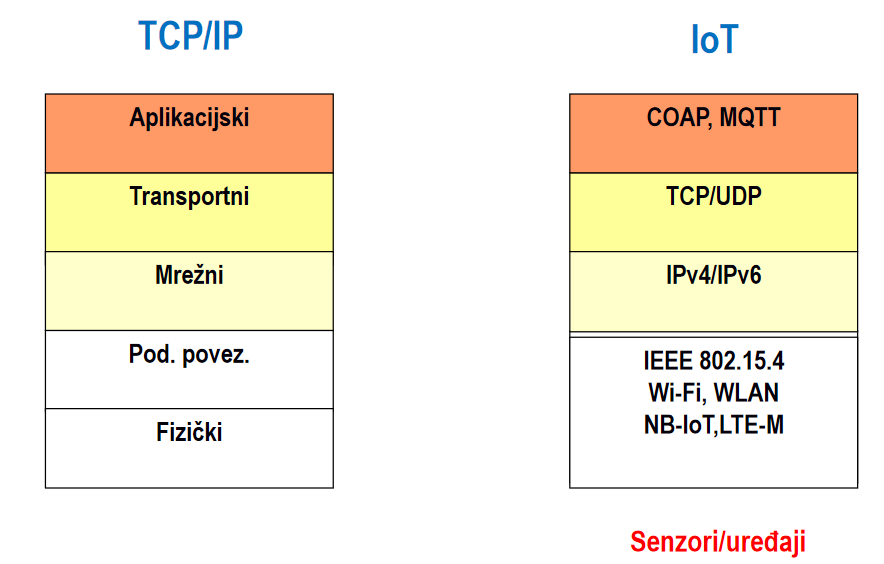
\includegraphics[width=11cm]{images/iot-stack.png}
    \caption{Protokolni složaj Interneta stvari\citep{InternetStvari}}
    \label{fig:iotstack}
\end{figure}

\section{Sloj uređaja}
Sloj uređaja je bazni sloj u Internetu stvari. Umrežavanjem tih uređaja i korištenjem njihovih senzorskih i aktuatorskih sposobnosti nam omogućava razvoj cjelokupnog sustava Interneta stvari. Uređaji se sastoje od nekoliko komponenti: napajanja, radio primopredajnika, senzora, analogno-digitalnih pretvornika koji dolaze kao zasebni moduli te mikroprocesora, memorije i razvojne pločice kao jedan jedinstveni uređaj. Postoje i već potpuno integrirani uređaji koji sadrže sve prije spomenute module na jednoj razvojnoj pločici. Prikaz modula uređaja nalazi se na sljedećoj slici.
\begin{figure}[htb]
    \centering
    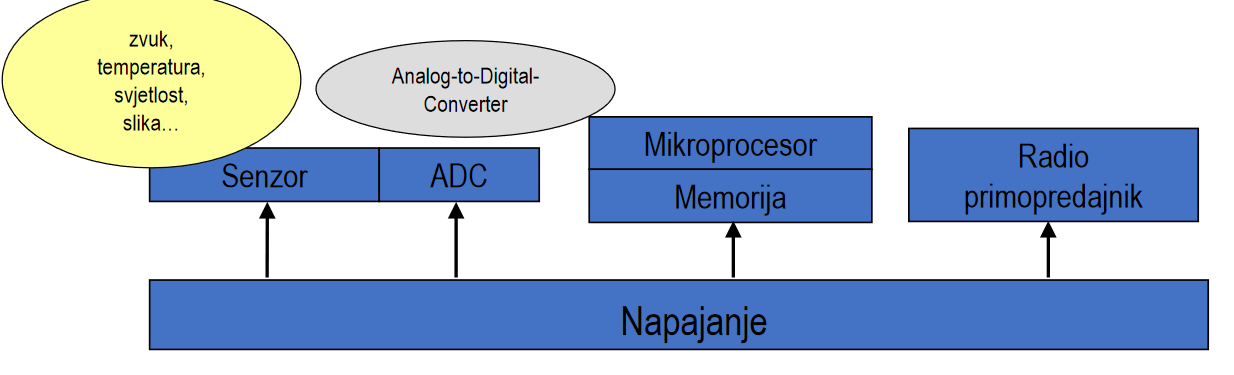
\includegraphics[width=14cm]{images/devicemodule.png}
    \caption{Moduli uređaja Interneta stvari\citep{InternetStvari}}
    \label{fig:devicemodule}
\end{figure}

Kod upotrebe Internet stvari uređaja postoji nekoliko zahtjeva koji se razlikuju s obzirom na primjenu. Neki od zahtjeva su: izrazito male dimenzije, mala potrošnja energije, niska cijena i umrežavanje na načelu samoorganizacije. Male dimenzije su potrebne kako bi uređaji djelovali neinvazivno na prostor u kojem se nalaze. Mala potrošnja energije je bitan zahtjev jer dio uređaja je mobilno te nema stalan izvor napajanja već koristi baterije koje nemaju veliki kapacitet ili solarne ćelije čija stopa punjenja nije visoka. Zbog energetske učinkovitosti uređaji imaju ograničenu procesorsku moć te je memorijski kapacitet ograničen. Najveća potrošnja energije se dešava na komunikacijskim modulima čija snaga signala otpada s kvadratom udaljenosti. Svi ti zahtjevi se trebaju uzeti u obzir tijekom planiranja kako bi se mogao utvrditi potreban uređaj za namijenjenu primjenu.

U nastavku će biti opisane senzorske pločice, komunikacijski modul te analizirani pristupni uređaji od kojih su neki potpuno integrirani kao jedna razvojna pločica.

\subsection{Senzorske pločice}
Uloga senzorskih pločica je očitavanje vanjskih fizičkih stvari što je jedna od glavnih mogućnosti sustava Interneta stvari. Senzori prisutni na pločicama omogućuju opažanje različitih vanjskih fizičkih pojava poput: temperature, prisutnosti, pokreta, zvuka, koncentracije plinova, magnetskih polja i protoka vode. Integracija tih pločica s mikrokontrolerima omogućuje procesiranje tih opažanja. Primjer senzorske pločice s mogućnošću očitanja razine buke, temperature i luminacijskog intenziteta je prikazan na sljedećoj slici.
\begin{figure}[htb]
    \centering
    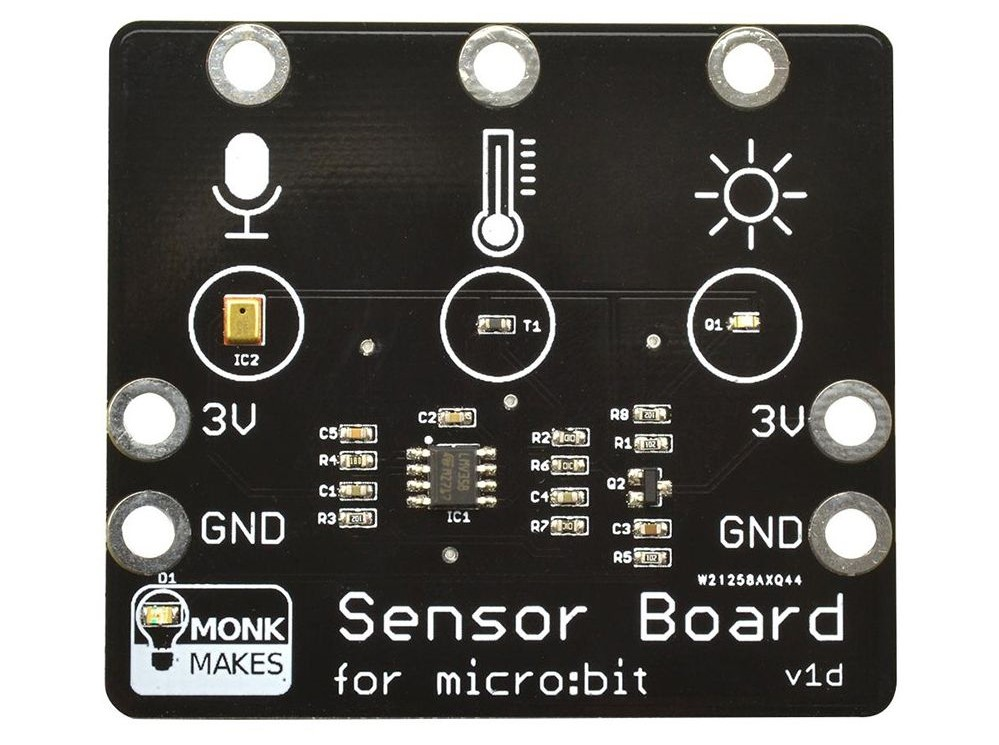
\includegraphics[width=5.5cm]{images/sensor_board.jpg}
    \caption{Senzorska pločica s mogućnošću očitanja razine buke, temperature i luminacijskog intenziteta\citep{SensorBoard}}
    \label{fig:sensorboard}
\end{figure}

\subsection{Komunikacijski moduli}
Komunikacijski moduli omogućuju uređajima da se umreže u ostatak sustava čime se ostvaruje glavni zahtjev u Internetu stvarima što je povezanost i mogućnost komunikacije. Moduli potrebni za komunikaciju ovise o fizičkom sloju i o sloju podatkovne poveznice. Fizički sloj uvjetuje fizički medij u kojem se podaci prenose. Žičani mediji su: bakrena žica u kojem se radi o elektronima i optički kablovi gdje se informacije prenose fotonima. Bežični mediji su: optički, koji ne koriste kablove već usmjerene laserske snopove koji putuju kroz zrak i radio valove čije različite frekvencije koriste različiti protokoli sloja podatkovne poveznice. 

Sloj podatkovne poveznice čine protokoli koji u osnovi opisuju način komunikacije putem fizičkog sloja. Na ovom sloju heterogenost protokola je najprisutnija, posebno kod protokola koji koriste radio valove kao fizički medij. Ta heterogenost se javlja zbog različitih potreba i primjena u sustavima. Tako na ovom sloju imamo različite protokole koji će biti obrađeni u sklopu analize protokola podatkovne poveznice. U nastavku je prikazan komunikacijski modul za protokol ZigBee.
\begin{figure}[htb]
    \centering
    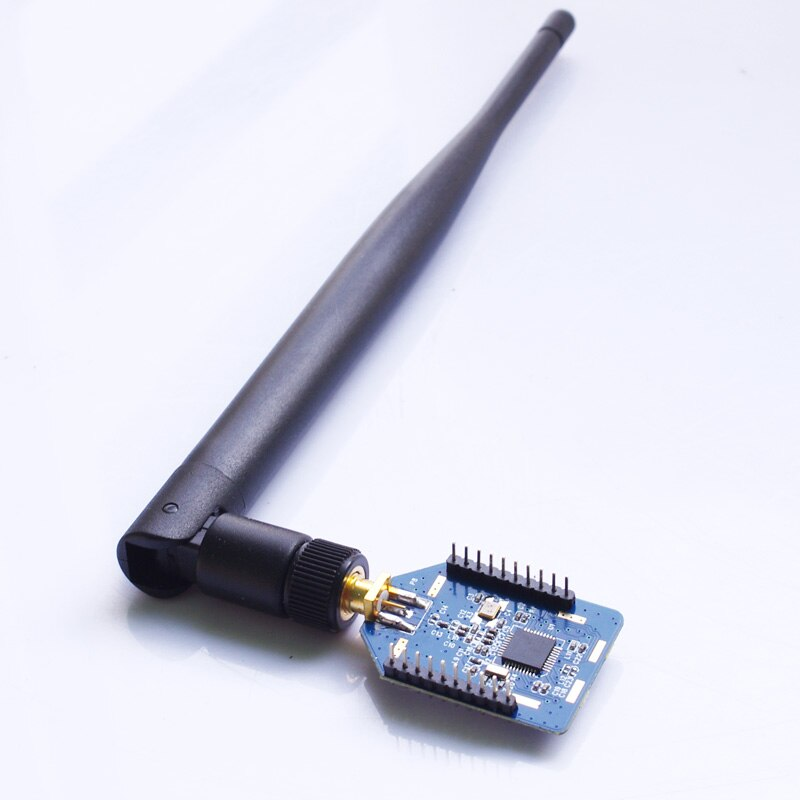
\includegraphics[width=6cm]{images/zigbee-module.jpg}
    \caption{ZigBee komunikacijski modul\citep{ZigBeemodule}}
    \label{fig:zigbeemodule}
\end{figure}

\subsection{Analiza pristupnih uređaja}
\subsubsection{Raspberry Pi 4 Model B}
Raspberry Pi je svojom pojavom na tržištu ponudio malo integrirano računalo za nisku cijenu čime je razvoj Interneta stvari postao pristupačniji za širu zajednicu. Zadnja verzija Pi računala je četvrta s time da sve tri prijašnje verzije su još uvijek u proizvodnji. Razlika između verzija je u procesorskoj snazi, radnoj memoriji, prisutnosti Ethernet i Wi-Fi modula te broju USB i HDMI priključaka. Na Raspberry Pi-u se izvršava GNU/Linux operativni sustav čime se uvelike olakšava razvoj aplikacija i dobiva podrška za postojeća programska rješenja. Na računalu se nalaze 40 priključnih pinova\engl{GPIO pins} koji omogućuju spajanje različitih senzorskih pločica, komunikacijskih modula, napajanja i zaslona čime se postiže visoka modularnost. Raspberry Pi je namijenjen kao stacionaran uređaj zbog njegove relativno visoke potrošnje energije s obzirom na integrirana računala s mikrokontrolerom što zahtjeva konstantan izvor napajanja putem strujnog adaptera. Neke od namjena su kao prilaz za ostale pametne uređaje zbog svoje procesorske snage, kao kontrolni centar sustav za pametan dom korištenjem platformi poput Home Assistanta, a spajanjem modula kamere Raspberry postaje nadzorna kamera. 

Raspberry Pi 4 Model B\citep{RPi4} je računalo koje poprima karakteristike stolnog računala. Tako sadrži Broadcom BCM2711, četverojezgreni Cortex-A72 (ARM v8) 64-bit SoC \engl{System on a chip}, 2, 4 ili 8 gigabajta radne memorije, gigabitni Ethernet priključak, Wi-Fi modul te 2 micro-HDMI priključka koji podržavaju do 4K 60Hz monitore. Te specifikacije dozvoljavaju korištenje RPi4 kao malo stolno računalo, a ne samo kao ugradbeno računalo s nekoliko senzora. Podrška za programske jezike koji se koriste za razvoj nije ograničen s obzirom na to da uređaj može izvršavati GNU/Linux operativni sustav. Na sljedećoj slici je prikazan Raspberry Pi 4.
\begin{figure}[htb]
    \centering
    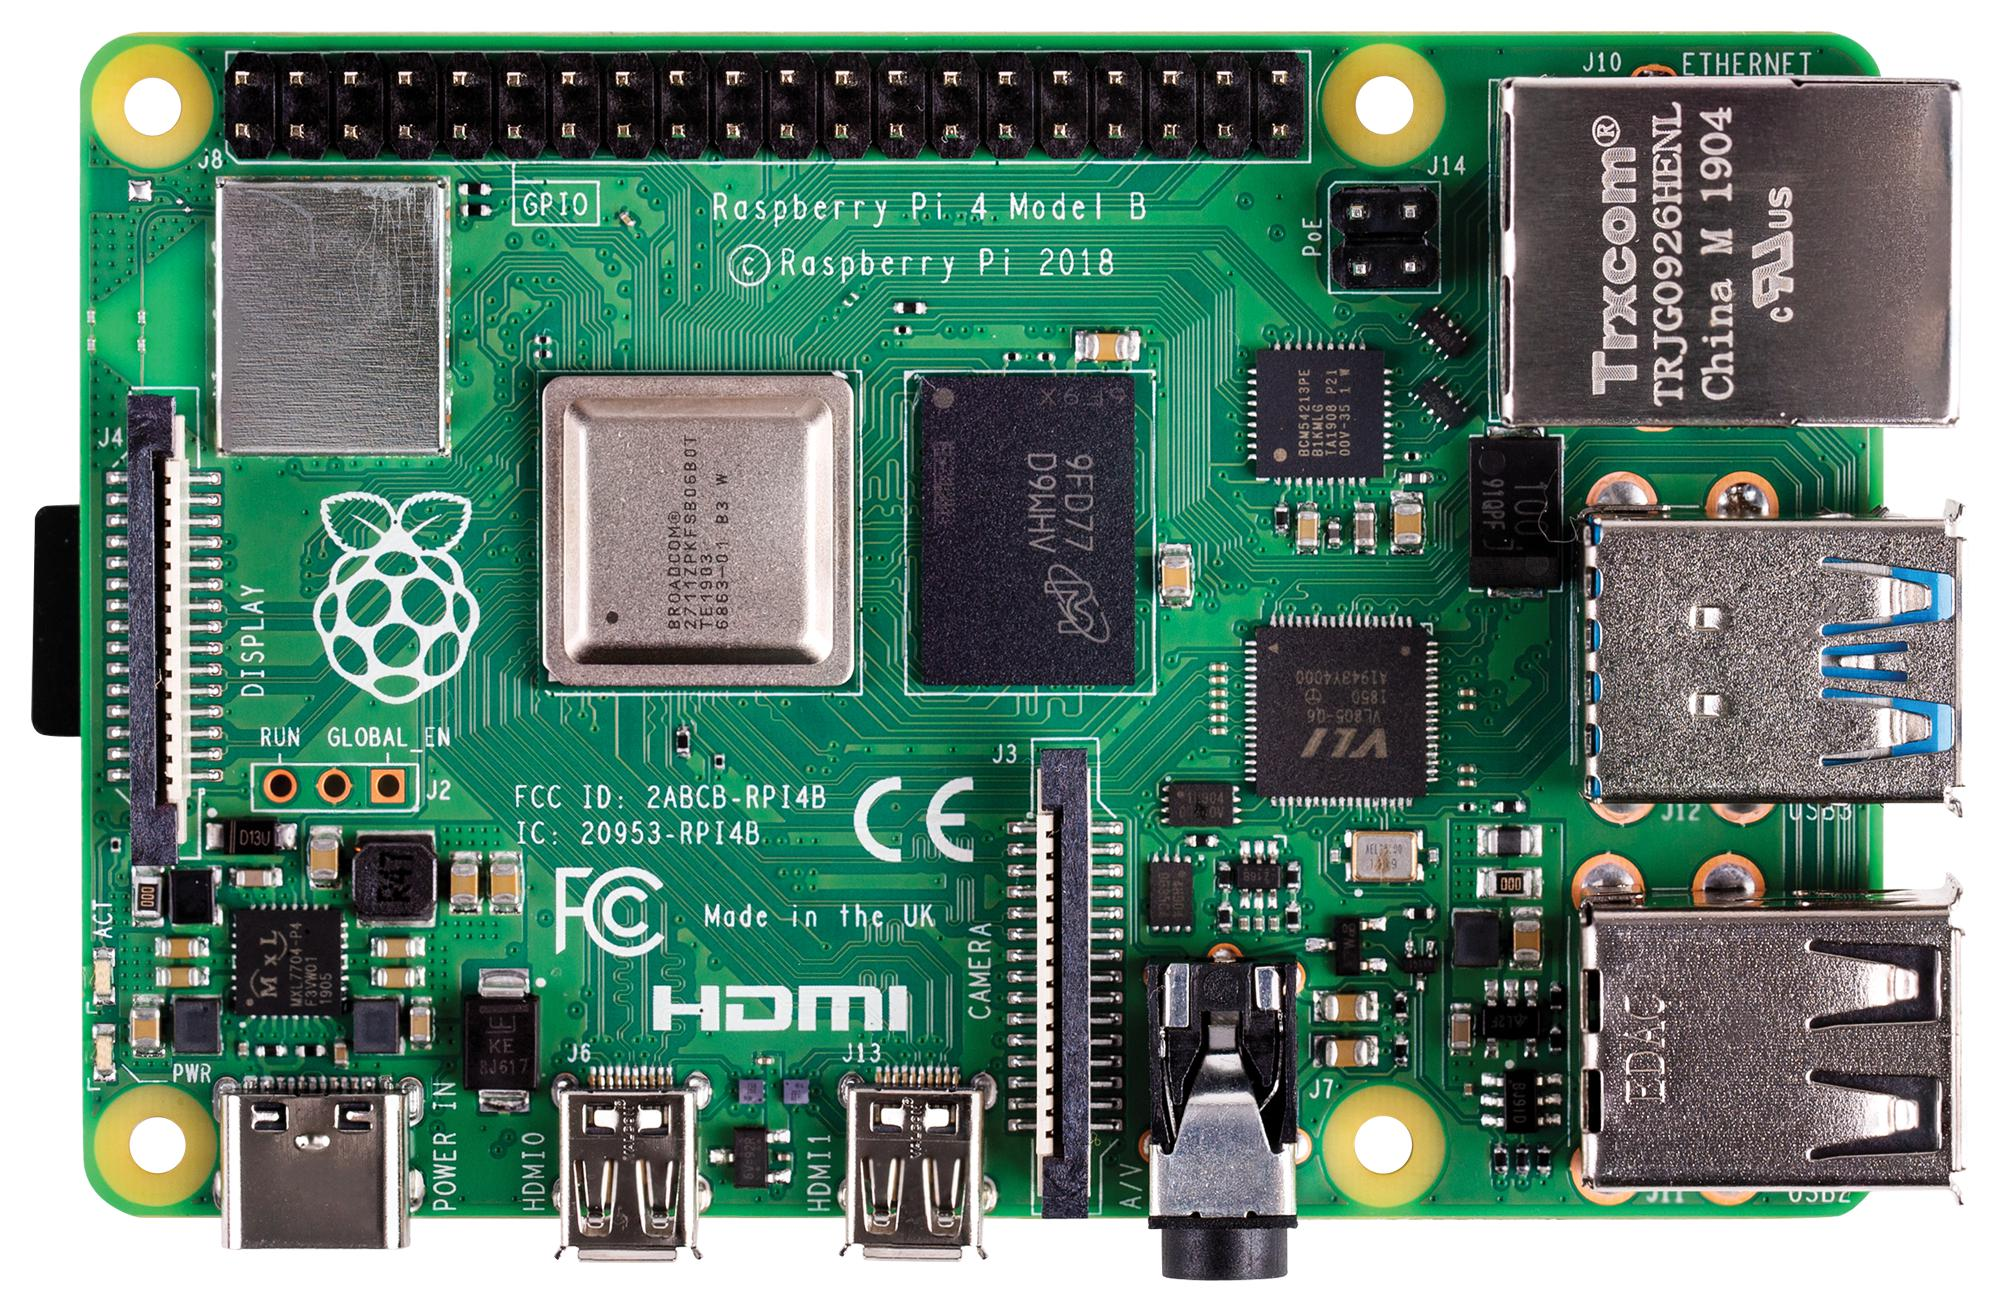
\includegraphics[width=8.5cm]{images/rpi4.jpg}
    \caption{Raspberry Pi 4 Model B\citep{RPi4Img}}
    \label{fig:rpi4}
\end{figure}

\subsubsection{Raspberry Pi Pico}
Raspberry Pi Pico\citep{RPiPico} je malo integrirano računalo s mikrokontrolerom niske cijene. Pico koristi RP2040 mikrokontroler čime se uvelike smanjuje potrošnja energije, ali i procesorska snaga samog računala čija radna frekvencija iznosi 133MHz s dvije jezgre. Sadrži 264KB SRAM-a te 2MB brze memorije čime je veličina izvršavajućih programa uvelike ograničena. Pico je veličine 21x51mm te tako uz svoju malu potrošnju energije dozvoljava da bude korišten za mobilne potrebe, a sa svojim 26 priključnih pinova dopušta visoku razinu modularnosti. Pristup uređaju se izvodi putem jednog micro-USB 1.1 priključka ili putem UART pinova, ali nema ugrađenih komunikacijskih modula te ako se želi omogućiti pristup mreži potrebno je koristiti zasebne module. Napajanje se provodi putem USB priključka ili putem vanjske baterije spojene na odgovarajuće pinove. Raspberry Pi Pico je ograničen na jednostavne senzorske i aktuatorske primjene zbog svoje ograničene procesorske brzine i kapaciteta pohrane podataka. Podrška za programske jezike koji se koriste za razvoj uređaja je ograničen na MicroPython, CircuitPython, C/C++ te Arduino programski jezik. Uređaj je prikazan na sljedećoj slici.
\begin{figure}[htb]
    \centering
    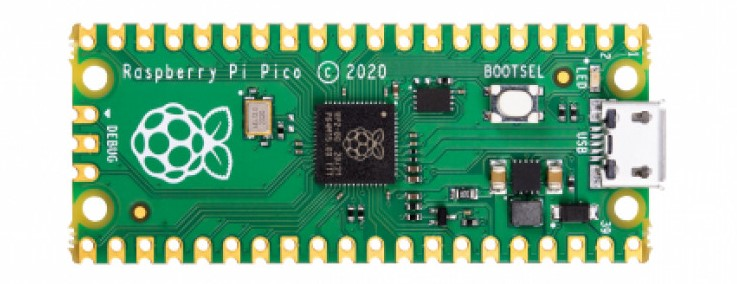
\includegraphics[width=5cm]{images/rpipico.jpg}
    \caption{Raspberry Pi Pico\citep{RPiPicoImg}}
    \label{fig:rpipico}
\end{figure}

\subsubsection{Arduino Uno Rev3}
Arduino je jedan od najvećih proizvođača malih razvojnih integriranih računala s mikrokontrolerom koji sadrži različite vrste tih računala koja se razlikuju u dimenzijama, priključcima i cijeni. Arduino Uno Rev3\citep{ArduinoUno} je jedno od tih integriranih računala koje je u svojoj prvoj verziji populariziralo i omogućilo jednostavan i jeftin razvoj za Internet stvari sustave. Shema cijele pločice je sklopovlje otvorenog izvora te je moguće pronači taj isti uređaj od drugih proizvođača. Treća revizija donosi 8 bitni ATmega328P mikrokontroler koji radi na frekvenciji od 16MHz sa 2KB SRAM-a te 32KB programabilne brze memorije. Na pločici se nalazi 20 priključnih pinova od kojih je 14 digitalnih te 6 analognih, uz jedan USB priključak putem kojeg se napaja i jedan zaseban priključak za napajanje. Zbog svoje otvorene i dobro dokumentirane sheme za ovaj uređaj postoji mnoštvo različitih senzorskih pločica i komunikacijskih modula koje je potrebno priključiti ako želimo povezati uređaj na mrežu. Glavna namjena Arduino Una je za brz razvoj jednostavnih Internet stvari rješenja te zbog svoje pristupačnosti je moguće pronaći mnoštvo gotovih projekta kako za senzorska tako i za aktuatorska rješenja. Podrška za programske jezike koji se koriste za razvoj uređaja je ograničen na C/C++ te Arduino programski jezik. Na sljedećoj slici je prikazan uređaj. 
\begin{figure}[htb]
    \centering
    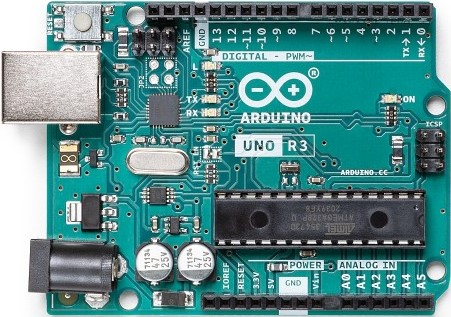
\includegraphics[width=6.8cm]{images/arduinouno.jpg}
    \caption{Arduino Uno Rev3\citep{ArduinoUno}}
    \label{fig:arduinouno}
\end{figure}

\subsubsection{Libelium Waspmote}
Waspmote\citep{Waspmote} je bežična senzorska platforma otvorenog koda posebno usmjerena na implementaciju načina rada s malom potrošnjom koja omogućuje čvorovima senzora da budu potpuno autonomni s prispojenom baterijom. Životni vijek jednog čvora može trajati od 1 do 5 godina, ovisno o radnom ciklusu i korištenim komunikacijskim modulima. Waspmote se temelji na modularnoj arhitekturi gdje je ideja integrirati samo module potrebne kako bi se optimizirao rad uređaja. Podržani moduli čine mnoštvo komunikacijskih, podatkovnih modula te senzorskih pločica. Waspmote sadrži 8-bitni ATmega1281 mikrokontroler koji radi na frekvenciji od 14.74MHz, SRAM od 8KB, 128KB programibilne brze memorije te podršku za SD kratice i mini USB priključak. Jedini programski jezik za razvoj je C++. Na sljedećoj slici je prikazan Libelium Waspmote.
\begin{figure}[htb]
    \centering
    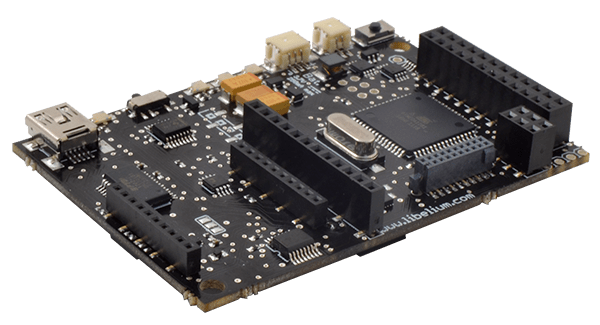
\includegraphics[width=8.9cm]{images/waspmote.png}
    \caption{Libelium Waspmote\citep{Waspmote}}
    \label{fig:waspmote}
\end{figure}

\subsubsection{ESP32}
Razvijen od strane Espressif Systema, ESP32\citep{ESP32} je malo integrirano računalo s mikrokontrolerom niske cijene. ESP32 dolazi s integriranim komunikacijskim modulima za Wi-Fi 802.11 b/g/n i Bluetooth s podrškom za BLE(Bluetooth Low Energy). Na pločici se nalazi dvojezgreni Tensilica Xtensa LX6 mikroprocesor s radnom frekvencijom do 240MHz, SRAM od 512KB, 4MB programabilne memorije, jedan micro USB priključak te 34 priključnih pinova. Napajanje se provodi putem USB priključka ili putem vanjske baterije spojene na odgovarajuće pinove. ESP32 je kod primjene najviše zastupljen kod mobilnih primjena zbog svoje niske potrošnje energije i malih dimenzija. Podrška za programske jezike koji se koriste za razvoj uređaja je ograničen na  MicroPython, CircuitPython, Lua, C/C++ te Arduino programski jezik. Prikaz ESP32 računala proizvedenog od strane Joy-IT-a je prikazan na sljedećoj slici.
\begin{figure}[H]
    \centering
    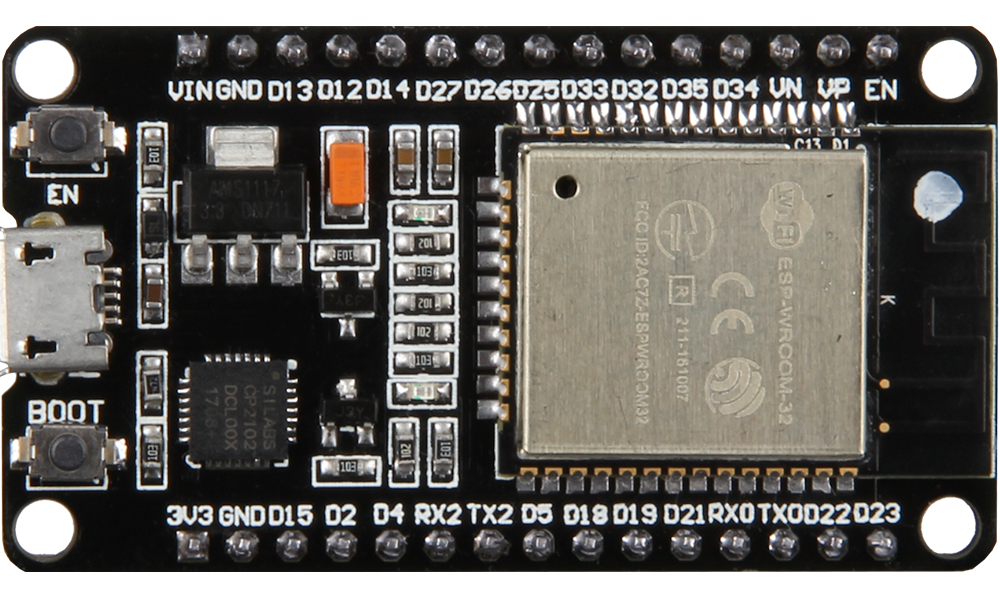
\includegraphics[width=4.8cm]{images/esp32.png}
    \caption{Joy-IT NodeMCU-ESP32\citep{ESP32Img}}
    \label{fig:esp32}
\end{figure}

\subsubsection{Pycom FiPy}
Pycom FiPy\citep{Fipy} je malo integrirano računalo temeljeno na ESP32 integriranom računalu. Uz sve prije navedene karakteristike i funkcionalnosti ESP32, FiPy sadrži 8MB programabilne memorije i integrirane komunikacijske module za LoRa, Sigfox i LTE-M. Kao i ESP32 FiPy se koristi za pretežito mobilne primjene zbog velikog broja integriranih bežičnih komunikacijskih modula koji dozvoljavaju velike udaljenosti od baznih prilaza što je posebno izraženo ako se koristi komunikacija putem Sigfoxa čiji domet je do 50 kilometara, LoRa čiji domet je do 40 kilometara i LTE-M čiji domet je do 10 km. Na sljedećoj slici je prikazan Pycom FiPy.
\begin{figure}[htb]
    \centering
    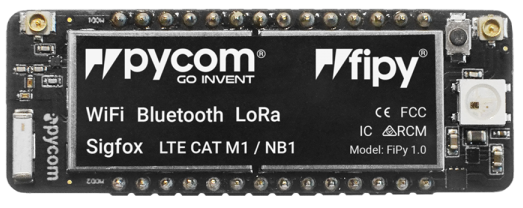
\includegraphics[width=5.5cm]{images/fipy.png}
    \caption{Pycom FiPy\citep{Fipy}}
    \label{fig:fipy}
\end{figure}


\subsection{Usporedba sigurnosnih mehanizama i primjena}
Kako bi komunikacija pristupnih uređaja prema vanjskim poslužiteljima bila sigurna potrebno je korištenje kriptografskih algoritama. Ti algoritmi zahtijevaju brzu procesnu snagu što nije slučaj za sve prije navedene uređaje osim Raspberry Pi 4 Model B koji ima četverojezgreni procesor radne frekvencije od 1.5GHz. Zato kao ispomoć u kriptografskim postupcima na pločicama se također nalazi i zasebni koprocesor za izvođenje kriptografskih algoritama ili podrška za sklopovsko ubrzanje određenih kriptografskih algoritama. Tako ESP32 i Pycom FiPy nude podršku za sklopovsko ubrzanje algoritama SHA, RSA i AES uz generator nasumičnih brojeva, Libelium Waspmote nudi podršku za kriptografske biblioteke za algoritme AES, RSA, MD5 i SHA iako nije navedena podrška za sklopovsko ubrzanje ili koprocesor. Arduino Uno Rev3 ne nudi nikakvu posebnu podršku za kriptografske algoritme iako neke verzije Una drugih proizvođača nude podršku za koprocesor za kriptografske algoritme. To je i slučaj s Raspberry Pi Picom gdje drugi uređaji temeljeni na Pico RP2040 mikroprocesoru imaju dodatan koprocesor na pločici. Raspberry Pi 4 Model B se približava poziciji stolnog računala te zbog svoje procesorske snage nema potrebe za dodatnim koprocesorima i na njemu se mogu izvoditi svi kriptografski postupci. Zato ako postoji potreba da uređaj samostalno obavlja zadatke i potrebno je osigurati komunikaciju između tog uređaja i bazne stanice ili poslužitelja najbolje je koristiti uređaje: Raspberry Pi 4 Model B, ESP32 i Pycom FiPy, dok Raspberry Pi Pico i Arduino Uno Rev3 je najbolje koristiti kao integrirano senzorsko računalo koje je dodatno putem priključnih pinova ili USB-a povezano sa snažnijim uređajem.

Primjena svih navedenih uređaja ovisi o njihovim izvorima napajanja, veličini, podršci za komunikacijske module i procesorskoj snazi. Ako gledamo procesorsku snagu i izvor napajanja tu dolazimo do pitanja energetske učinkovitosti uređaja koja ograničava mogućnost upotrebe baterija kao izvora napajanja. Tako će se Raspberry Pi 4 Model B koristiti kao stacionaran pametan uređaj s vanjskim napajanjem, dok ostali navedeni uređaji imaju mogućnost biti baterijski napajani što dozvoljava mobilnu primjenu. Zbog svoje velike procesorske snage Raspberry Pi 4 Model B može djelovati kao poslužitelj i prilaz za ostale pametne uređaje dok su ostali uređaji većinom ograničeni na jednostavne senzorske i aktuatorske primjene. Svi navedeni uređaji imaju podršku za vanjske komunikacijske module te nisu ograničeni na tom području iako neki od uređaja dolaze s već integriranim modulima što dozvoljava brz, jednostavan i jeftin razvoj.

\section{Fizički sloj i sloj podatkovne poveznice}
 Fizičkog sloj se definira fizičkim medijem kojem se prenose podaci. Postoje dvije vrste kategorije medija, žičani i bežični na kojima se zatim temelje protokoli podatkovne poveznice. Uloga fizičkog sloja je da definiraju fizički medij koji se koristi u komunikaciji, svojstva tog medija poput frekvencije koja će se koristiti u radiovalnoj komunikaciji, sinkronizaciju, pakete i linijske kodove dok sloj podatkovne poveznice definira strukturu paketa, automate stanja, adresiranje, sinkronizaciju, kontrolu protoka i korekciju grešaka. Na ovim slojevima se nalazi velika heterogenost protokola zbog različitih potreba u sustavima Interneta stvari. Heterogenost protokola je najizraženija u bežičnoj komunikaciji zbog različitih potreba u dometu komunikacije, brzini prijenosa informacija, latenciji i mobilnosti uređaja. Sve ove potrebe su posebno izražene jer upotrebom bežične komunikacije proširujemo mogućnosti primjena uređaja, dok žičane komunikacije uglavnom ograničavamo za potrebe komunikacije prilaza i vanjskih servisa zbog stabilne i brze komunikacije. U nastavku se analiziraju i uspoređuju samo neki od protokola fizičkog sloja i sloja podatkovne poveznice temeljenih na bežičnim tehnologijama.

\subsection{Analiza protokola}
\subsubsection{IEEE 802.11 Wi-Fi}
IEEE 802.11 Wi-Fi je porodica bežičnih komunikacijskih protokola temeljenih na radiofrekvencijskom prijenosu. Varijante protokola Wi-Fi su jedni od najbolje zastupljenih komunikacijskih protokola zbog svoje pojave na tržištu s uređajima kojima je cilj bio mobilna uporaba poput prijenosnih računala i mobilnih telefona. Kroz godine se počela pojavljivati potreba za bržim prijenosom podataka, manjom latencijom i mogućnošću povezivanja više uređaja na jednu baznu stanicu \engl{access point} što je dovelo i do razvoja različitih standarda koji svi čine jednu porodicu protokola. U tablici su prikazani različiti standardi te frekvencije koje koriste i maksimalna propusnost koja se može postići.
\begin{table}[H]
    \centering
    \caption{Varijante protokola Wi-Fi}
    \begin{tabular}{| c | c | c | c |} 
    \hline
    \textbf{Standard} & \textbf{Ime} & \textbf{Frekvencije} & \textbf{Maksimalna propusnost}\\
    \hline\hline
    802.11a & Wi-Fi 2 & 5 GHz & 54 Mbps\\
    \hline
    802.11b & Wi-Fi 1 & 2.4 GHz & 11 Mbps\\ 
    \hline
    802.11g & Wi-Fi 3 & 2.4 GHz & 54 Mbps\\ 
    \hline
    802.11n & Wi-Fi 4 & 2.4 i 5 GHz & 600 Mbps\\ 
    \hline
    802.11ac & Wi-Fi 5 & 2.4 u 5 GHz & 1.3 Gbps \\ 
    \hline
    802.11ax & Wi-Fi 6 & 2.4 i 5 GHz & 10-12 Gbps\\ 
    \hline
    802.11ah & Wi-Fi HaLow & EU: 866 MHz & 347 Mbps\\ 
    \hline
    \end{tabular}
    \label{tab:wifi}
\end{table}

IEEE 802.11i je dopuna na IEEE 802.11 \emph{Wired Equivalent Privacy} (WEP) sigurnosni mehanizam definiran u originalnom 802.11 standardu koji je zbog svoje slabih sigurnosnih svojstva neadekvatan standard. IEE 802.11i također nosi naziv i \emph{Wi-Fi Protected Access II} (WPA2). WPA2 je trenutno najkorišteniji za sigurnost komunikacija vezanih uz protokole Wi-Fi. Prethodni WPA je također uz WEP prestao biti korišten u široj upotrebi zbog pronađenih sigurnosnih propusta vezanih uz slabe kriptografske algoritme korištene u šifriranju prometa. WPA3 je zadnji sigurnosni standard koji nudi poboljšanja u autentifikacijskom postupku i šifriranju prometa te će biti zadani standard za Wi-Fi 6 komunikaciju. U nastavku je prikazana tablica koja prikazuje razlike u svim sigurnosnim mehanizmima. Zbog raširenosti u nastavku će se promatrati sigurnosni mehanizmi WPA2.
\begin{table}[H]
    \centering
    \caption{Usporedba sigurnosnih Wi-Fi standarda}
    \begin{tabular}{| M || S | S | X | X |} 
    \hline
                              & \textbf{WEP} & \textbf{WPA} & \textbf{WPA2} & \textbf{WPA3}\\
    \hline\hline
    \textbf{Razvijen godine}         & 1997. & 2003. & 2004. & 2018.\\
    \hline
    \textbf{Razina sigurnosti}& Jako niska & Niska & Visoka & Jako visoka\\ 
    \hline
    \textbf{{Šifriranje}}     &  RC4 & TKIP & AES-CCMP & AES-CCMP AES-GCMP\\ 
    \hline
    \textbf{Veličina ključa}  & 64 bita \hspace{0.2cm}128 bita & 64 bita\hspace{0.2cm} 128 bita &  128 bita & 128 bita \hspace{1cm}256 bita\\ 
    \hline
    \textbf{Autentifikacija}  & Otvoreni pristup Dijeljeni ključ & PSK AAAK & PSK \hspace{1cm}AAAK & AES-CCMP AES-GCMP\\ 
    \hline
    \textbf{Integritet}       & CRC-32 & 64 bitni MIC & AES-CCMP & SHA-2\\ 
    \hline
    \end{tabular}
    \label{tab:wpa}
\end{table}

WPA2 uvodi koncept \emph{Robust Security Network} (RSN), koji se definira kao bežična sigurnosna mreža koja omogućuje kreiranje sigurnih bežičnih konekcija naziva \emph{Robust Security Network Associations} (RSNA). RSNA omogućava sigurnosne mehanizme napredne autentifikacije korisnika, upravljanje kriptografskim algoritmima, povjerljivost podataka, autentifikacija i integritet izvora podataka te zaštitu od napada ponavljanjem. RSNA koristi dvije autentifikacijske metode koje se koriste kako bi se odvijalo izvođenje kriptografskih ključeva za autentifikacija i integritet podataka. \emph{Pre-Shared Key} (PSK) se koristi u nekomercijalnim mrežama gdje svi korisnici koji pristupaju mreži koriste jedan ključ, tj. lozinku. \emph{Authentication, Authorization, and Accounting Key} (AAAK) koji se pristupnoj točki dostavlja putem \emph{Extensible Authentification Protocol} (EAP) koji omogućuje autentifikaciju korisnika putem identiteta gdje svaki korisnik ima svoje pristupne podatke i koristi se većinom u komercijalnim mrežama. 

Tri različite komponente RSNA su: krajnji uređaji koji pristupaju mreži (STA) \engl{stations}, pristupna točka (AP) \engl{access point} i autentifikacijski poslužitelji (AS). U nastavku se promatraju pet faza za uspostavu i raskid veze, a na slici \ref{fig:psk} su prikazane faze korištenjem PSK autentifikacijske metode.
\begin{enumerate}
    \item\textbf{Otkrivanje:} STA identificira AP za mrežu s kojom želi uspostaviti komunikaciju. STA locira AP primanjem jednog od AP-ovih periodičnih \emph{Beacon} okvira ili slanjem \emph{Probe} zahtjeva. Nakon što STA identificira AP, dolazi do izmjenjivanja okvira za pregovor oko komunikacijskih parametara. Na kraju prve faze su uspostavljeni kriptografski protokoli za povjerljivost i integritet podataka, autentifikacijska metoda i način distribucije ključeva.
    \item\textbf{Autentifikacija:} U slučaju metode korištenjem AAAK u ovoj fazi se izvodi međusobna autentifikacija STA i AP-a. Autentifikacijski okviri prolaze kroz AP do AS-a kako bi se korištenjem EAP-a mogla odviti autentifikacija. AP blokira sve okvire STA koji nisu autentifikacijski dok se ne izvrši autentifikacija STA.Kada se autentifikacija izvrši AAAK se sprema na STA i AP. Metoda korištenjem PSK nema ovu fazu zbog korištenja jednog ključa za pristup.
    \item\textbf{Generiranje i distribucija ključeva:} Tijekom ove faze AP i STA izvode nekoliko operacija koje generiraju kriptografske algoritme za daljnju komunikaciju. To se izvodi kroz dvije vrste rukovanja: četverostruko rukovanje i rukovanje grupnim ključevima.
    \item\textbf{Zaštićeni prijenos podataka:} STA i AP izmjenjuje podatke sigurnim putem korištenjem sigurnosnih politika i kriptografskih ključeva uspostavljenih tijekom prve tri faze. Jer se sigurni prijenos odvija samo između STA i AP-a, potrebno je zasebno zaštiti podatke tijekom ostatka prijenosa.
    \item\textbf{Raskid konekcije:} STA i AP prekidaju svoju sigurnu vezu i brišu podatke o svojoj međusobnoj povezanosti\citep{NIST}.
\end{enumerate}
\begin{figure}[H]
    \centering
    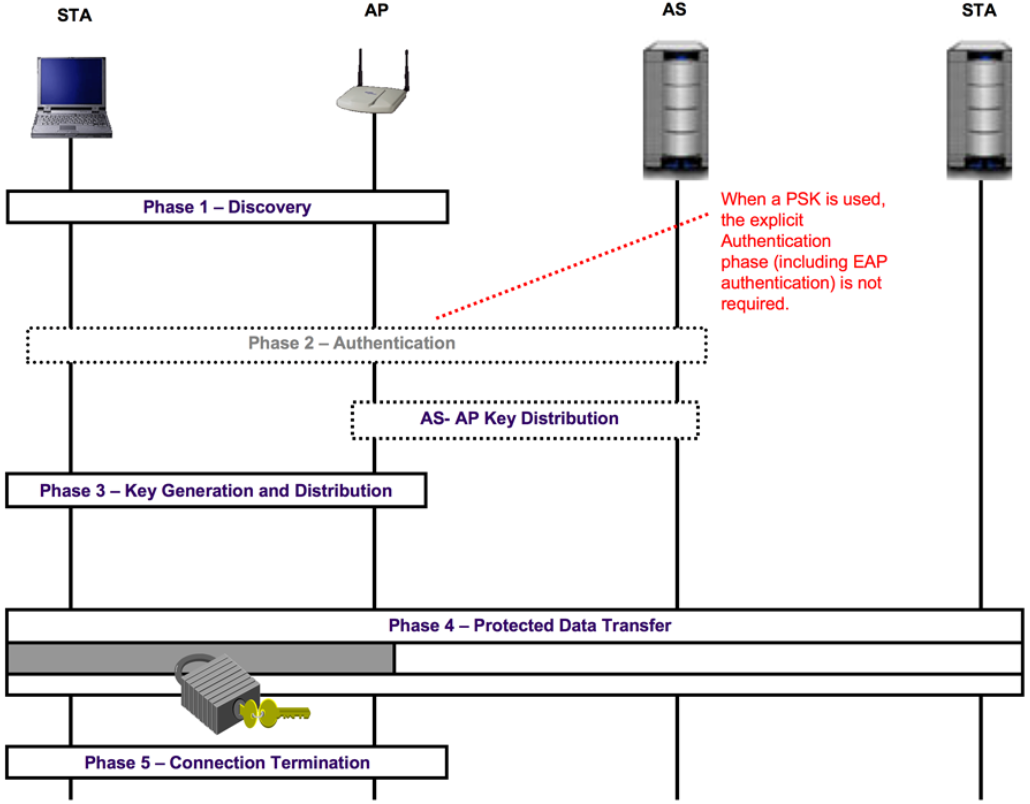
\includegraphics[width=11cm]{images/psk.png}
    \caption{Faze uspostava i raskida veze korištenjem PSK metode\citep{NIST}}
    \label{fig:psk}
\end{figure}

\subsubsection{Bluetooth Low Energy}
\emph{Bluetooth Low Energy} (BLE) je bežični protokol male snage te je jedan od dva protokola pod Bluetooth nazivom. Drugi protokol je Bluetooth Classic koji se koristi za kontinuiranu komunikaciju velikog skupa podataka na maloj udaljenosti te kao takav je korišten u Internetu stvari, ali za potrebe stacionarnih uređaja sa stalnim izvorom napajanja koji kontinuirano šalju podatke. BLE koristi periodični prijenos manjih podatkovnih paketa te u trenucima kada ne sudjeluje u razmjeni podataka je u stanju mirovanja što uvelike doprinosi smanjenju potrošnje energije. Tako se omogućuje razvoj manjih mobilnih uređaja koji mogu biti pokretani duže vrijeme na maloj bateriji. 

Na fizičkom sloju BLE koristi ISM \engl{Industrial, Scientific, and Medical} radiofrekvencijski pojas na frekvenciji od 2.4GHz. Brzina podatkovnog prijenosa je 1Mbps za verzije 4.2 ili starije, a za verzije 5 i novije može postići do 2Mbps. Udaljenost na kojoj uređaji mogu komunicirati ovisi o preprekama koje se nalaze, vrsti antene, kućištu i orijentaciji uređaja, ali teoretska maksimalna udaljenost je između 100 i 400 metara.

Topologija BLE mreže podrazumijeva dvije vrste uređaja:
\begin{description}
    \item[Centralni uređaji:]imaju veću procesnu snagu i odgovorni su za kontroliranje perifernih uređaja. Na njima se izvode aplikacije posebno izrađene za interakciju s perifernim uređajima. Neki od primjera centralnih uređaja su: pametni telefoni, tableti i računala. 
    \item[Periferni uređaji:]mala integrirana računala koja obnašaju zadaću opažanja koristeći senzore te prikupljene podatke šalju na centralne uređaje za obradu. Neki od primjera perifernih uređaja su: pametni satovi, nosivi medicinski uređaji i industrijski termostati.
\end{description}

Kako bi se mogla odvijati komunikacija između centralnih i perifernih uređaja prvo je potrebno uspostaviti konekciju postupkom koji se naziva uparivanje \engl{pairing}. Uparivanje se odvija u dvije ili tri faze, tijekom koji uređaji izmjenjuju podatke potrebne za autentifikaciju, poput ključeva i ulazno/izlaznih sposobnosti. Treća faza je neobavezna te se dešava u slučaju da će uređaji uspostaviti vezu \engl{bond}. Vezivanje \engl{bonding} je proces u kojem uređaji spremaju autentifikacijske podatke koje su izmijenili tijekom prvobitnog uparivanja kako bi se uklonila potreba za ponovnim uparivanje tijekom ponovne uspostave komunikacije. Tijekom prve faze uređaji razmjenjuju informacije o identitetu i sposobnostima uređaja i komunikacija nije šifrirana. Druga faza je posvećena generiranje i izmjeni ključeva te je tijekom ove faze moguć napad \emph{man-in-the-middle} napad gdje napadač može preuzeti kontrolu nad uređajem i podacima koje se prenose. Kod treće faze uparivanja uređaji generiraju set ključeva za autentifikaciju kod budućih uspostava veza. Ti ključevi mogu biti par potpisnih ključeva za razlučivanje konekcije \engl{Connection Signature Resolving Keys}, koji se koriste za digitalni potpis podataka, te ključevi za razlučivanje identiteta \engl{Identity Resolving Keys}, koji se koriste za generiranje privatnih MAC adresa i pretraživanje. Kriptografski algoritam koji se koristi za šifriranje prometa je AES \engl{Advanced Encryption Standard} sa 128 bitnim ključem izveden tijekom postupka uparivanja. Prikaz postupka uparivanja je prikazan na sljedećoj slici.
\begin{figure}[H]
    \centering
    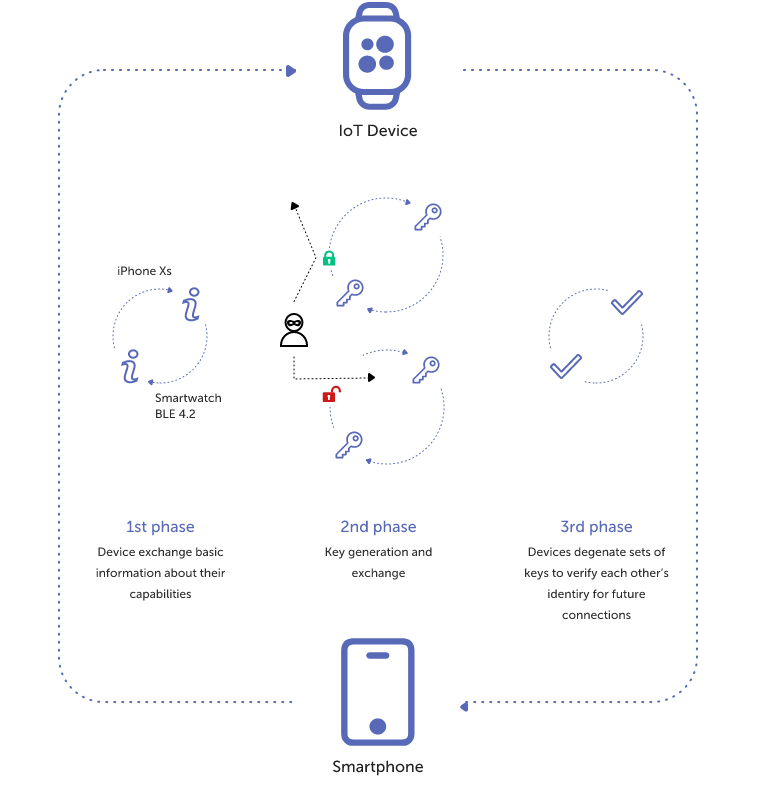
\includegraphics[width=13cm]{images/ble.png}
    \caption{Uparivanje uređaja protokolom BLE \citep{Kacherovska2019Aug}}
    \label{fig:ble}
\end{figure}

BLE podržava dvije vrste konekcija \emph{Legacy} i \emph{Secure}. Legacy konekcije mogu biti implementirane za verzije 4.0, 4.1 i 4.2. Uređaji razmjenjuju vrijednost privremenog ključa \engl{Temporary Key} i koriste tu vrijednost kako bi generirali kratkoročni ključ \engl{Short Term Key} koji se zatim koristi za autorizaciju konekcije. BLE Legacy konekcije su nesigurne, ali mogu biti osigurane s određenim metodama uparivanja. Secure konekcije su predstavljane s verzijom 4.2 i nisu kompatibilne sa starijim verzijama protokola. Ove konekcije implementiraju algoritam eliptičke krivulje Diffie-Hellman (ECDH) za generiranje ključeva i donose kompleksniji proces autentifikacije ključima. Tako se sprječava napad prisluškivanjem i uređaji mogu biti dodatno osigurani s određenim metodama uparivanja opisanim u nastavku.

\emph{Just Works} metoda uparivanja je zadana metoda za većinu BLE mreža. Kod Legacy konekcija vrijednost privremenog ključa tijekom druge faze uparivanja je postavljena na 0 i uređaji generiraju kratkoročni ključ na temelju te vrijednosti. Takva vrsta sparivanja je jako nesigurna i ne nudi nikakvu vrstu zaštite, već samo način za uspostavu veze. Ova vrsta uparivanja može biti kompleksna i pouzdana za osnovnu sigurnost konekcije kroz sljedeće korake:
\begin{enumerate}
    \item Korištenjem kriptografskog algoritma ECDH, oba uređaja generiraju privatni i javni par ključeva i izmjenjuju javni ključ.
    \item Uređaj koji prima zahtjev za konekcijom generira nasumičnu vrijednost i koristi tu vrijednost kako bi generirao potvrdnu vrijednost. Uređaj šalje obje vrijednosti uređaju koji je inicirao konekciju.
    \item Uređaj koji inicira konekciju generira vlastitu potvrdnu vrijednost s nasumičnom vrijednosti koju je primio od drugog uređaja. Uspoređuje vlastitu potvrdnu vrijednost s potvrdnom vrijednosti koju je dobio od drugog uređaja.
    \item Ako su vrijednosti identične, uređaji uspostavljaju vezu.
\end{enumerate}
Ova metoda nudi zaštitu od pasivnog prisluškivanja, ali ne i od \emph{man-in-the-middle} napada te se ne preporučuje za primjene gdje se razmjenjuju osjetljivi podaci. 

\emph{Out of Band} metoda uparivanja dozvoljava da se određeni podaci tijekom druge faze uparivanja šalju putem nekog drugog bežičnog protokola kako se ključevi ne bi razmjenjivali putem manje sigurnog protokola BLE ili kada uređaji razmjenjuju osjetljive podatke. Krajnja sigurnost ove metode ovisi o protokolu koji se koristi te se na taj način može spriječiti napadi pasivnim prisluškivanjem i \emph{man-in-the-middle} napadi.

\emph{Passkey} metoda uparivanja koristi korisnike kao dio procesa. Postoje različiti načini implementacije ove metode. Jedan od primjera je da uređaj generira lozinku od šest znamenki, koju tada korisnik treba unijeti na drugom uređaju. Na ovaj način se svaki uređaj ručno verificira od strane korisnika što zahtjeva da uređaji imaju neki oblik unošenja i prikazivanja podataka. Ovim načinom se sprječavaju napadi pasivnim prislušikavnjem i \emph{man-in-the-middle} napadi.

Metoda uparivanja numeričkom usporedbom je dostupna samo za Secure konekcije te također zahtjeva sudjelovanje korisnika. Nakon druge faze uparivanja uređaji koriste nasumične vrijednosti koje su prije razmijenili kako bi generirali šesteroznamenkastu vrijednost koju korisnik treba usporediti na oba uređaja. Ova metoda nudi zaštitu od \emph{man-in-the-middle} napada jer nijedan uređaj se ne može povezati na mrežu bez ručne verifikacije\citep{Kacherovska2019Aug}.


\subsubsection{LoRaWAN}
LoRaWAN \engl{Long Range Wide Area Network} je standard za bežičnu komunikaciju koji dozvoljava komunikaciju uređaja Interneta stvari preko velikih udaljenosti s minimalnom energetskom potrošnjom. LoRa i LoRaWAN su pojmovi koji se koriste naizmjenično iako definiraju različite slojeve Internet stvari složaja. LoRa definira fizički sloj dok LoRaWAN definira protokol i arhitekturu sustava. LoRa definira različite radiofrekvencijske pojase koji pripadaju ISM pojasevima. U Europi LoRa koristi frekvencije na pojasu oko 869MHz, dok u Sjevernoj Americi koristi 923MHz čime se javlja nekompatibilnost uređaja proizvedenih za ta dva tržišta. Domet komunikacije ovisi o monogo parametara poput naseljenosti područja u kojem se odvija komunikacija. Za urbana područja domet je oko 5km, predgrađa 10km, a u nenaseljenim područjima može dostići i do 80km.
LoRaWAN arhitektura se sastoji od: krajnjih čvorova (uređaja), LoRa prilaza, mrežnog poslužitelja i krajnjih aplikacija. Prikaz topologije LoRaWAN arhitekture je na sljedećoj slici.
\begin{figure}[H]
    \centering
    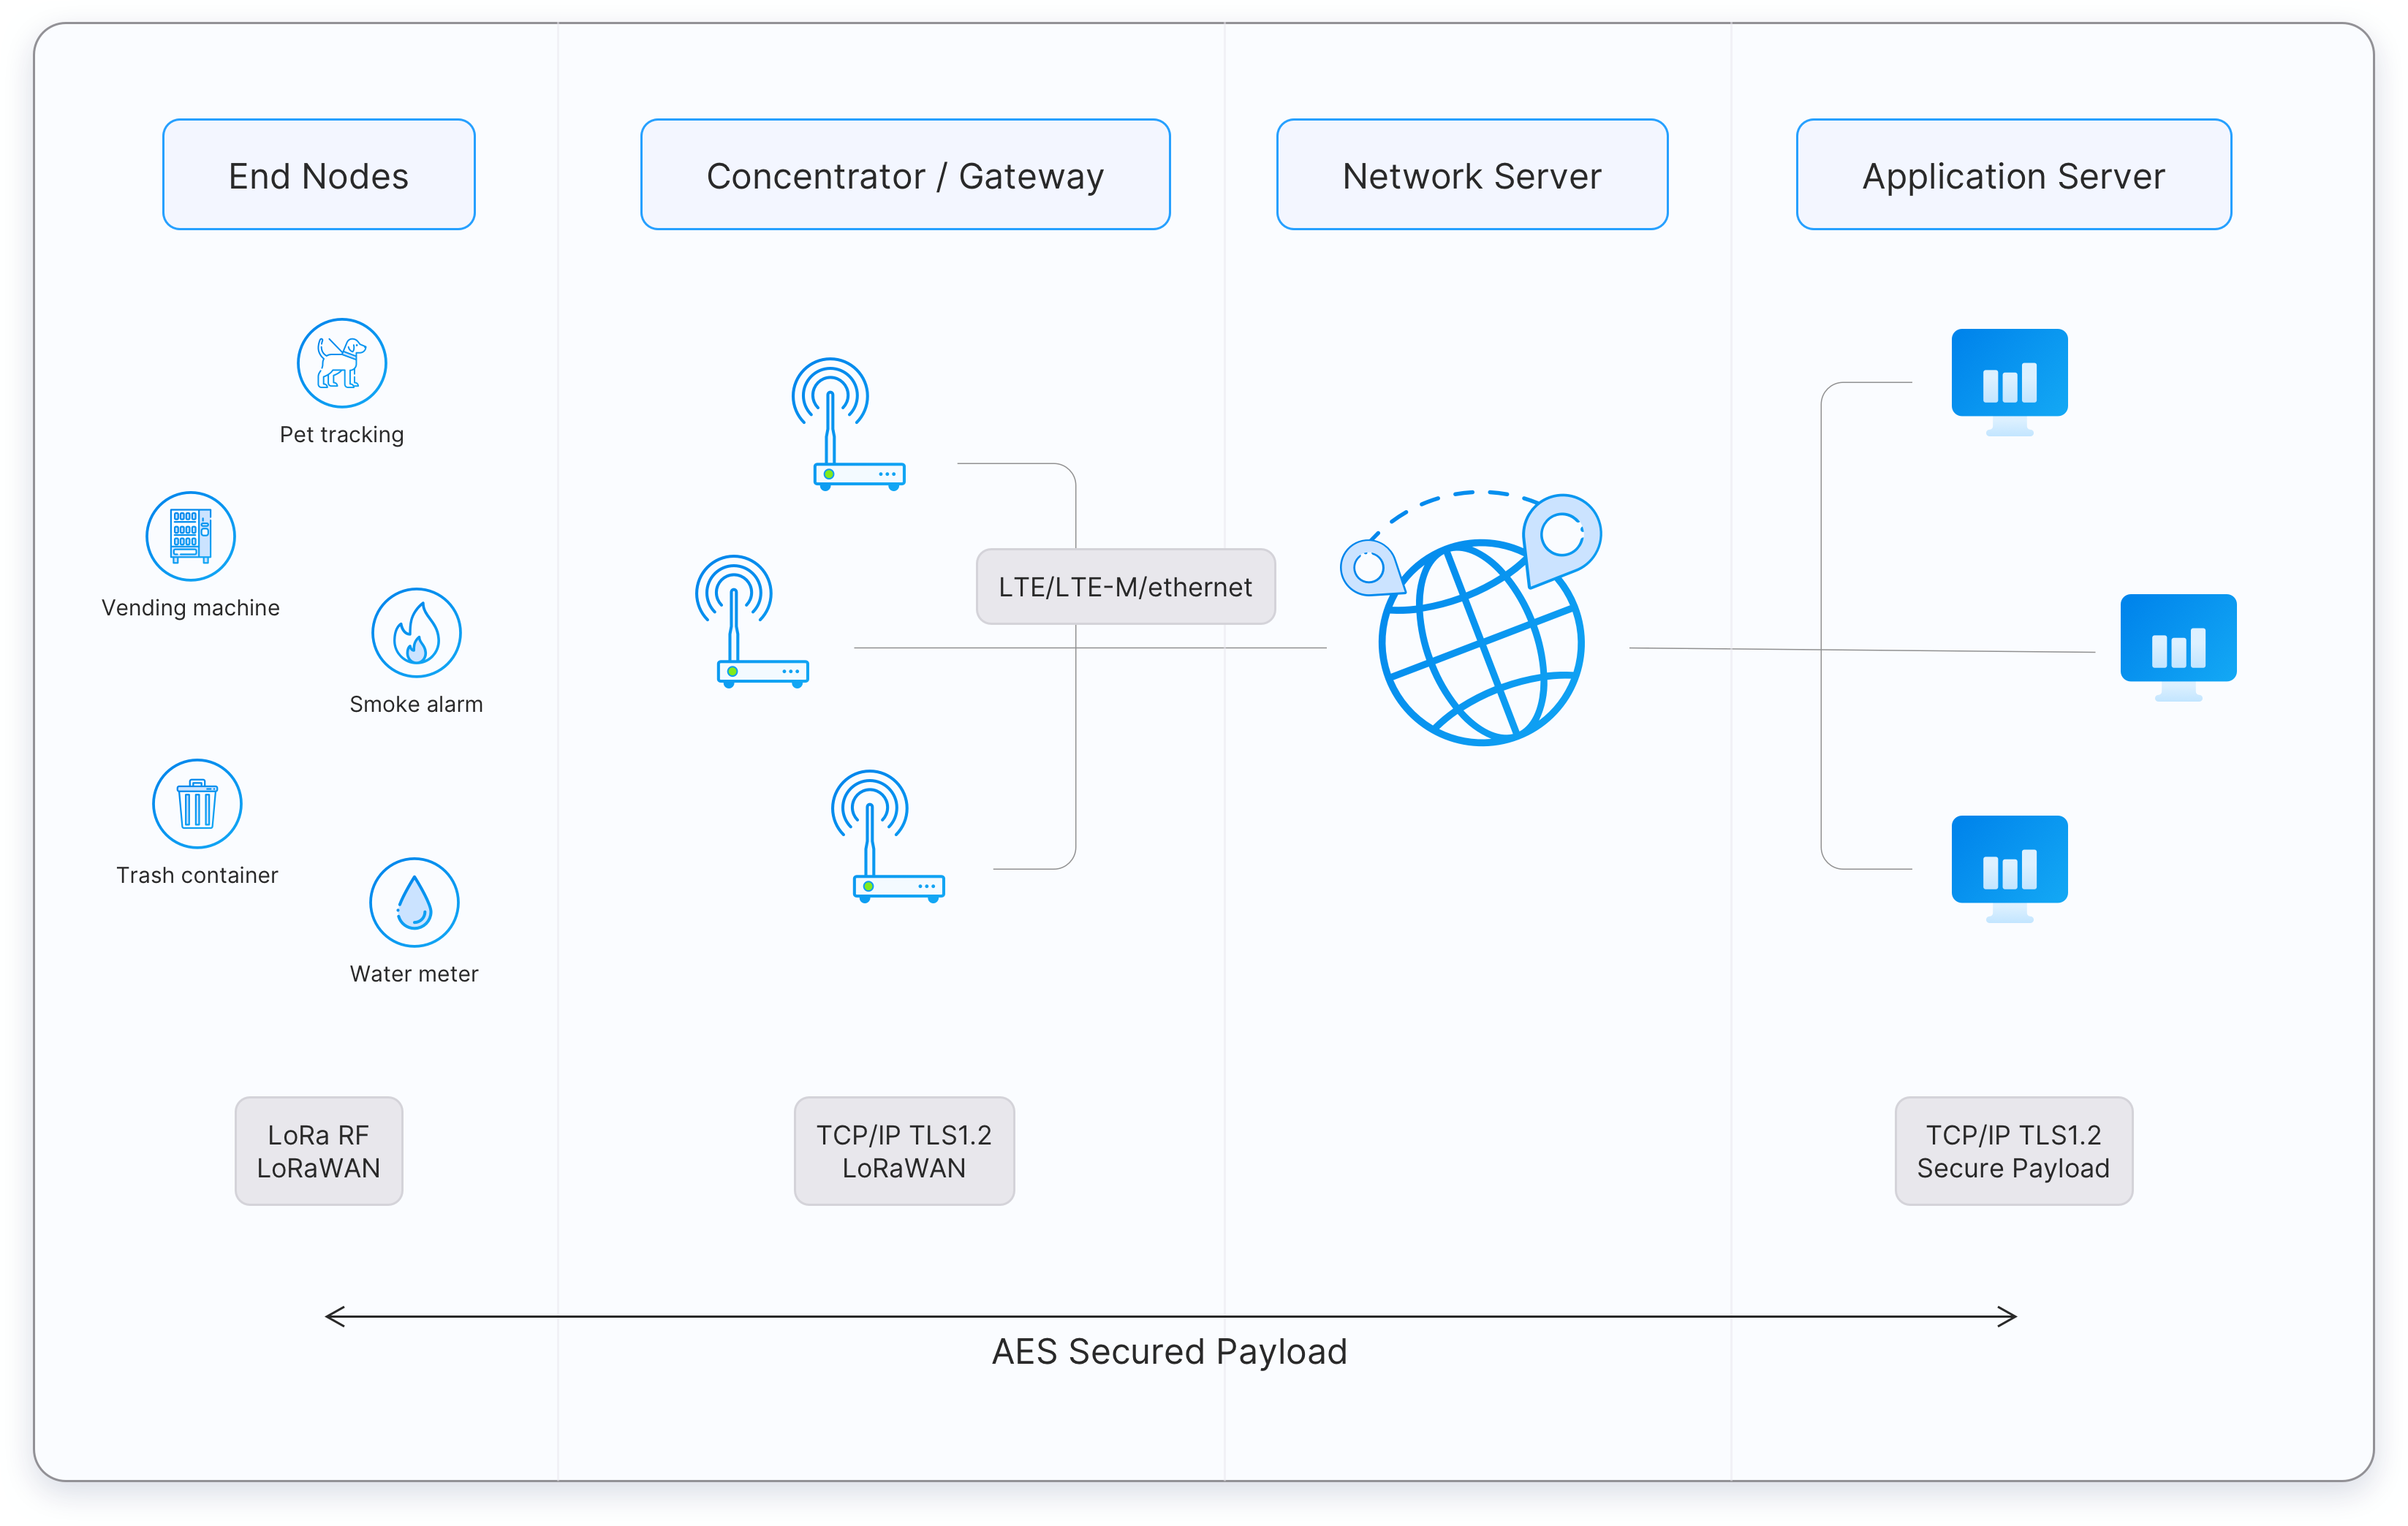
\includegraphics[width=11cm]{images/lorawan.png}
    \caption{Topologija LoRaWAN arhitekture\citep{LoraWANImg}}
    \label{fig:lorawan}
\end{figure}

Krajnji čvorovi mogu biti senzori ili aktuatori, često su napajani baterijama i imaju visoku razinu energetske učinkovitosti te tako mogu dugo funkcionirati na jednom punjenju. Postoje 3 kategorije čvorova. Klasa A je najučinkovitija te može primati poruke samo nakon uspješnog slanja poruke s uređaja. Klasa B nadograđuje klasu A i dodaje mogućnost primanja poruka u predodređenim intervalima. Klasa C može primati podatke samo kada ih ne šalje. Uređaji na mreži koriste sljedeće vrste adresa i identifikatora:
\begin{description}
    \item[DevEUI:]Jedinstveni identifikator formata EUI64 \engl{Extended Unique Identifier} adrese veličine 64 bita. Usporedivo s MAC adresama za TCP/IP uređaje.
    \item[DevAddr:]Adresa uređaja veličine 32 bita dodijeljena ili odabrana na mreži. Usporedivo s IP adresama za TCP/IP uređaje.
    \item[AppEUI:]Aplikacijski identifikator formata EUI64 adrese. Jedinstveno identificira aplikacijskog davatelja usluga uređaja. AppEUI se sprema na krajnji čvor prije nego se izvodi aktivacijski postupak za verzije prije 1.1.
    \item[JoinEUI:]Identifikator pristupnog poslužitelja formata EUI64 adrese. Jedinstveno identificira pristupnog poslužitelja. JoinEUI se sprema na krajnji čvor prije nego se izvodi aktivacijski postupak za verziju 1.1.
    \item[Fport:]Identificira vrata aplikacijskog procesa. Usporedivo sa TCP/UDP vratima za TCP/IP uređaje.
\end{description}

LoRa prilazi primaju LoRa poruke od krajnjih uređaja te samo prosljeđuju te podatke na mrežne poslužitelje. Prilazi su povezani na Internet putem drugih protokola poput Wi-Fi-a, Etherneta ili mobilnih mreža.

Mrežni poslužitelji upravljaju cijelom LoRaWAN mrežom. Zadaće poslužitelja su:
\begin{itemize}
    \item agregiranje svih dolaznih podataka s LoRa prilaza,
    \item usmjeravanje poruka na aplikacijske poslužitelje,
    \item konfiguraciju prilaza,
    \item optimiziranje brzine prijenosa podataka, vremena emitiranja i potrošnje energije na mreži,
    \item aktivaciju krajnjih uređaja,
    \item slanje potvrda o primljenim porukama.
\end{itemize}

Pristupni poslužitelj obrađuju pristupne zahtjeve krajnjih uređaja. Poslužitelj obavlja funkcije spremanja root kriptografskih ključeva, generira ključeve sjednice i prijenosi ključeve sjednice mrežnim i aplikacijskim poslužiteljima. Pristupni poslužitelj je uveden u LoRaWAN mrežu od verzije 1.0.4 i 1.1.

LoRaWAN 1.1 nudi nekoliko razina sigurnosti. Mrežni poslužitelj ne treba imati informaciju o sadržaju poruke koja se usmjeruje, a da nije relevantna za mrežu ili infrastrukturu. Zato postoje dva različita kriptografska 128 bitna ključa koji koriste algoritam za šifriranje AES i 2 ključa za provjeru integriteta poruka kod uređaja kako bi se postigla zaštita podataka na dvije razine. Ključevi korišteni nakon povezivanja uređaja na mrežu su sljedeći:
\begin{description}
    \item[SNwkSIntKey:]Ovo je ključ mrežne sjednice koji koristi uređaj za potvrdu integriteta svake primljene poruke putem \emph{Message Integrity Code} (MIC) provjere i za izračun MIC-a za pola odlazne poruke.
    \item[FNwkSIntKey:]Ovo je ključ mrežne sjednice koji koristi uređaj za izračun MIC-a cijelog ili dijela odlazne poruke.
    \item[NwkSEncKey:]Ovo je ključ mrežne sjednice koji koristi uređaj za šifriranje i dešifriranje dolaznih i odlaznih poruka MAC naredbi.
    \item[AppSKey:]Ovo je ključ aplikacijske sjednice koji koriste aplikacija i uređaj za šifriranje i dešifriranje poruka koje izmjenjuju.
\end{description}
Mrežni ključ sjednice (NwkSEncKey) se koristi za komunikaciju između krajnjeg čvora i mrežnog poslužitelja. Ključ potvrđuje integritet svake poruke putem \emph{Message Integrity Code} (MIC) provjere. Ta provjera je slična provjeri koristeći kontrolnu sumu uz razliku da onemogućuje neautorizirane promjene sadržaja poruke. Ova provjera se također koristi za mapiranje DevAddr na jedinstvene DevEUI i AppEUI. NwkSEncKey se nakon aktivacije čvora dijeli s mrežom.

Aplikacijski ključ sjednice (AppSKey) se koristi za šifriranje i dešifriranje sadržaja poruka. Sadržaj poruke je šifriran cijelim putem između čvora i aplikacijskog poslužitelja. Ovaj ključ se generira kao i NwkSkey nakon aktivacije čvora, ali samo čvor i aplikacijski poslužitelj imaju taj ključ, što omogućava potpunu tajnost podataka dok ne stigne do aplikacije.

Za aktivaciju čvora i pristupanje mreži kako bi se mogla odvijati komunikacija i kako bi se stvorili kriptografski ključevi se može odviti s dva različita postupka: ABP \engl{Activation By Personalization} i OTAA \engl{Over The Air Activation}.

ABP je najjednostavniji način za aktivaciju i pristup LoRa uređaja na mrežu. Dobavljač uređaja od davatelja mrežne usluge otkupi određeni raspon DevAddr adresa i opskrbi svoje uređaje s tim adresama. Nakon što se uređaj upali odmah je spreman za komunikaciju s prilazima. Koraci u postupku aktivacije su:
\begin{enumerate}
    \item Dobavljač uređaja otkupi mogućnost povezivanja od davatelja mrežnih usluga. AppSKey je generiran unaprijed.
    \item Davatelj mrežnih uređaja dostavlja NwkSkey i DevAddr za svaki DevEUI.
    \item Prije uporabe uređaja se opskrbljuje uređaje s: NwkSkey, AppSKey i DevAddr
    \item Kod prvog korištenja uređaja, nema nikakvog koraka za aktivacijom i pristupa uređaja mreži jer uređaji već mogu komunicirati s mrežom jer imaju sve potrebne informacije.
\end{enumerate}

OTAA je za razliku od ABP postupka kompliciraniji, ali dopušta pristup bilo kojoj mreži u blizini i ne zahtijeva poseban dogovor između dobavljača uređaja i davatelja mrežnih usluga. Postupak je različit za verziju 1.1 i ranije verzije, a ovdje će se gledati postupak aktivacije za verziju 1.1. Kako bi se sigurnim putem dobavili potrebni ključevi i adresa uređaja postupak koristi dva dodatna kriptografska ključa naziva AppKey i NwkKey koji uz DevEUI trebaju biti spremljeni na uređaju prije postupka aktivacije. To su kriptografski ključevi od 128 bita korišteni za kriptografski algoritam AES. Na pristupnom poslužitelju su spremljeni AppKey, NwkKey i DevEUI. Koraci u postupku aktivacije su prikazani na sljedećoj slici i opisani u nastavku.
\begin{figure}[H]
    \centering
    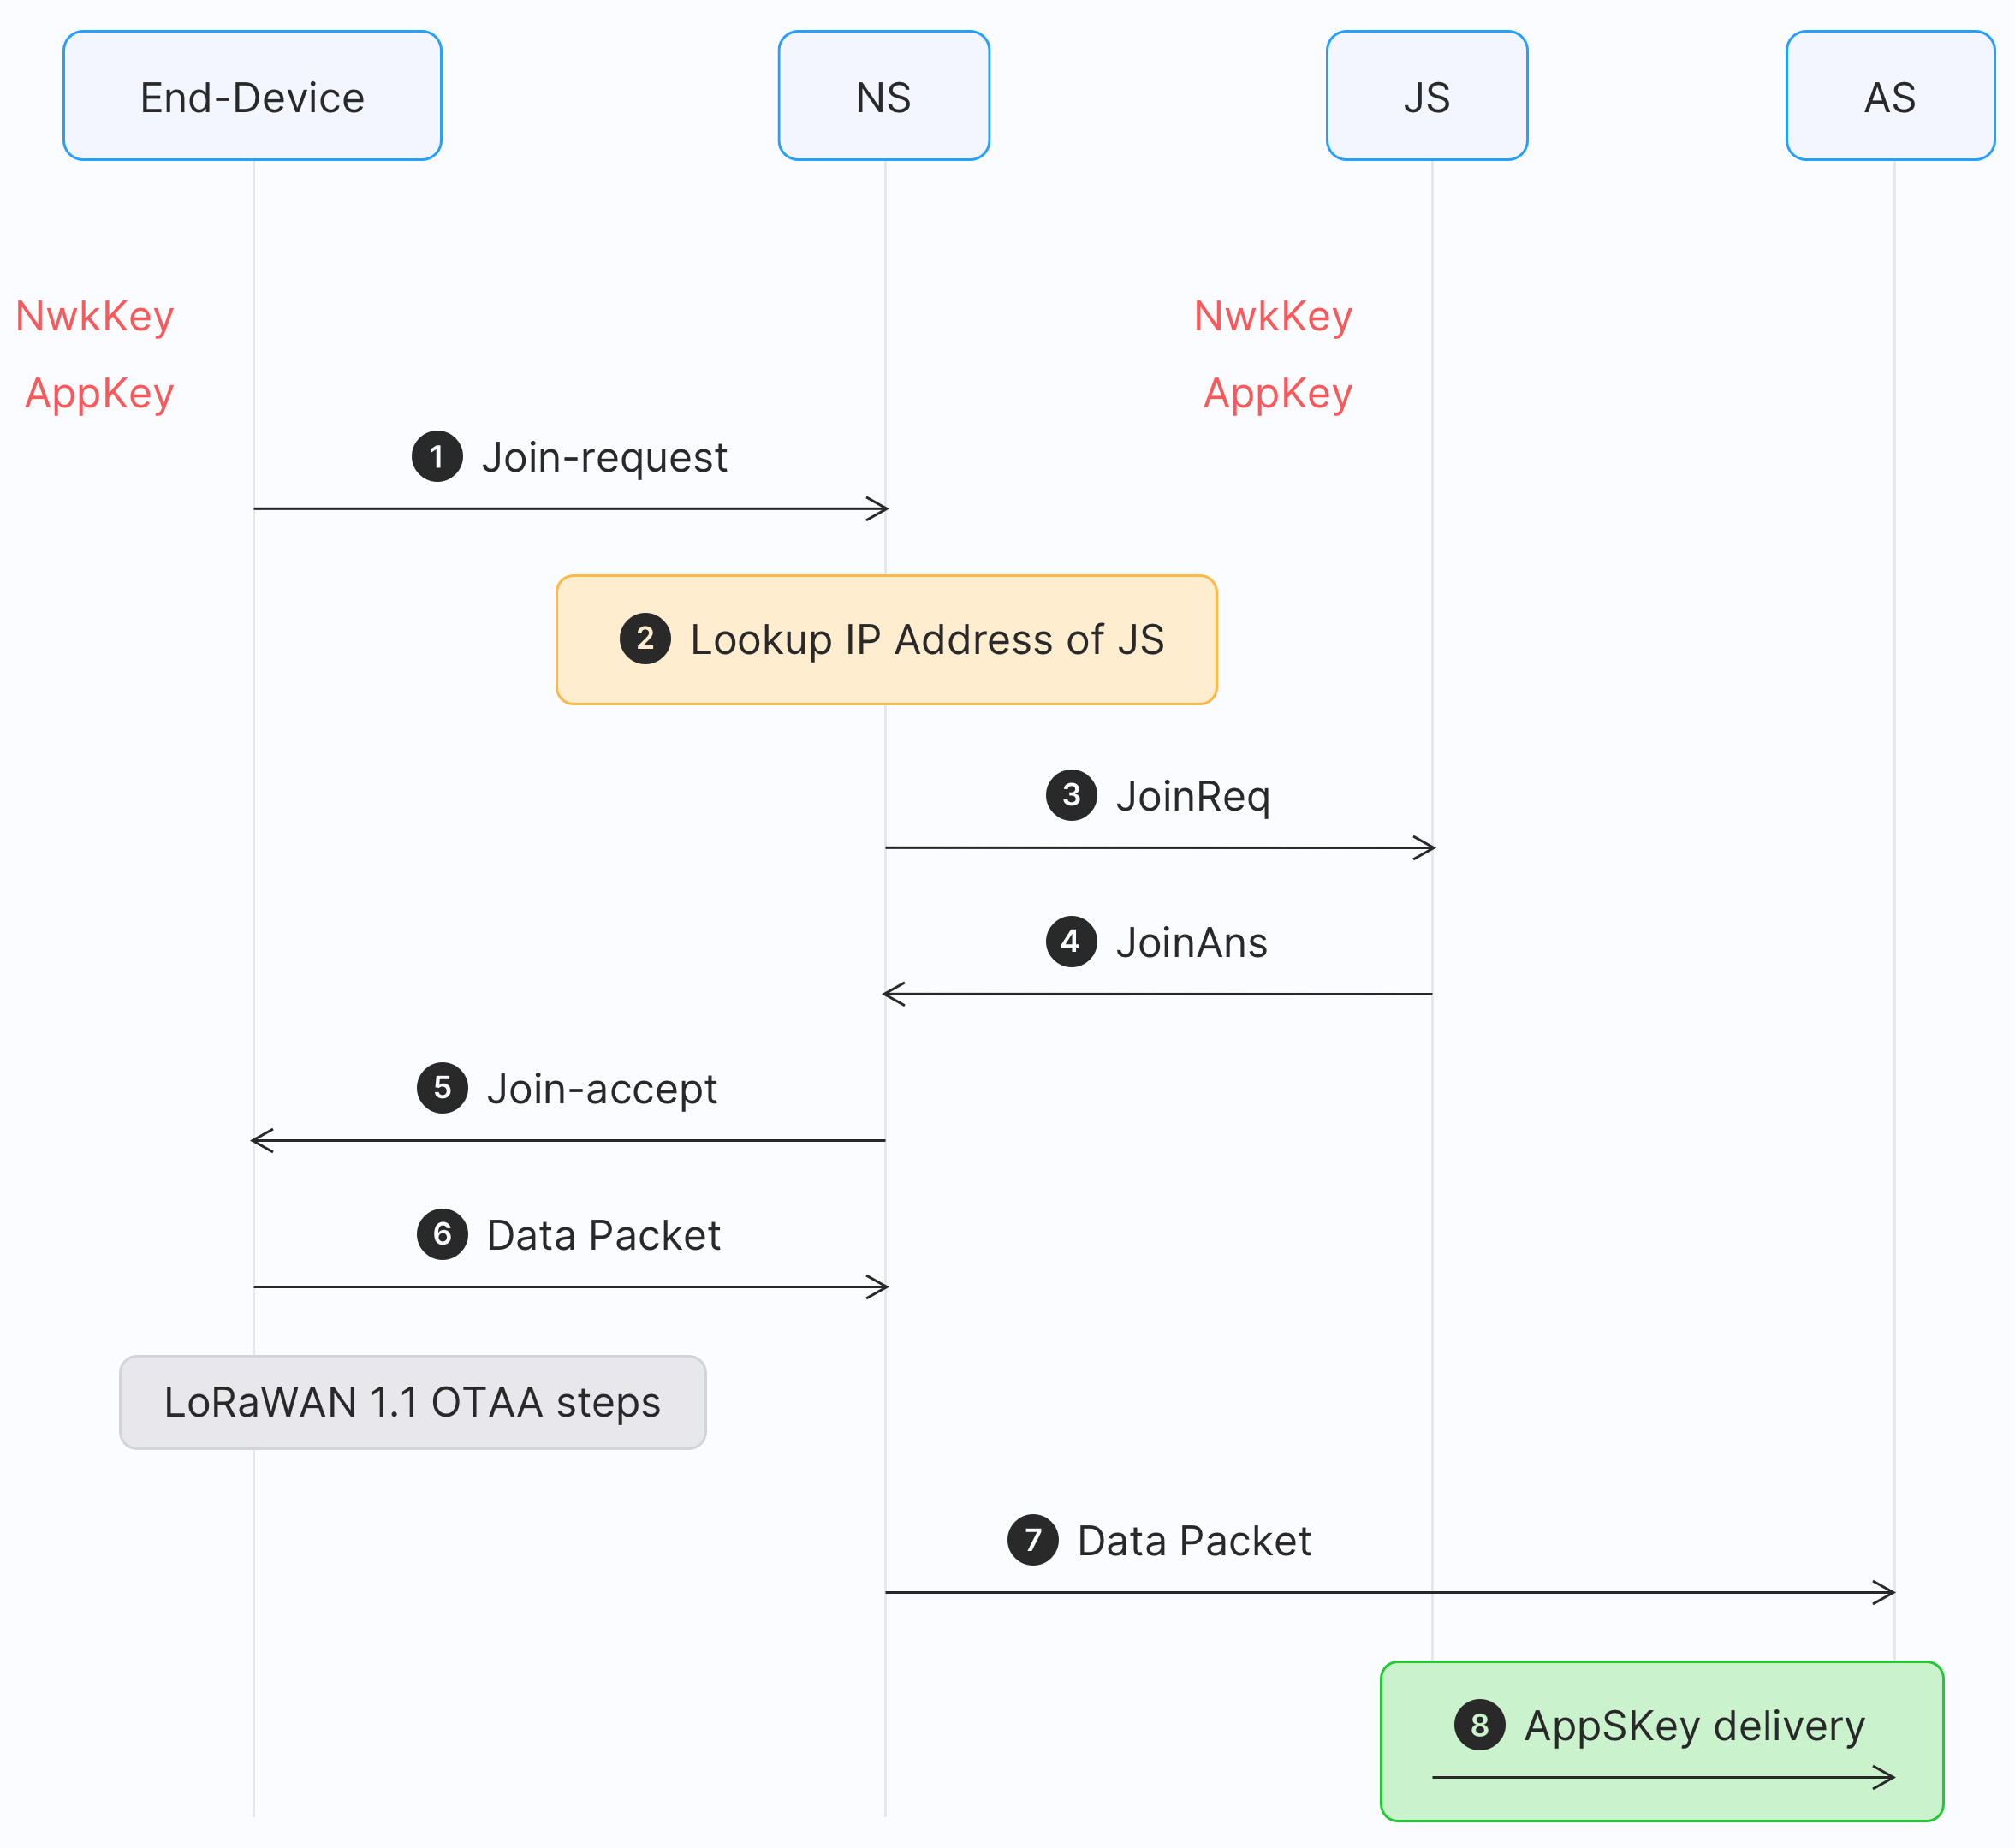
\includegraphics[width=8.8cm]{images/otaa.png}
    \caption{Tijek LoRaWAN 1.1 OTAA postupka\citep{LoRaWAN}}
    \label{fig:otaa}
\end{figure}
\begin{enumerate}
    \item LoRa uređaj šalje Join-request zahtjev potpisan s NwkKey. Zahtjev za pristup mreži sadrži JoinEUI, DevEUI i DevNonce. DevNonce je dvobitni brojač koji počinje s vrijednošću 0 i inkrementira se sa svakim Join-request zahtjevom, a koristi se za sprječavanje napada ponavljanjem. Ovaj zahtjev nije šifriran. Zahtjev LoRa prilazi prosljeđuju na mrežni poslužitelj.
    \item Mrežni poslužitelj koristi DNS kako bi doznao IP adresu pristupnog poslužitelja iz JoinEUI polja.
    \item Mrežni poslužitelj šalje JoinReq zahtjev na pristupni poslužitelj. Zahtjev sadrži Join-request zahtjev, MAC verziju, DevAddr i druge servisne informacije.
    \item Pristupni poslužitelj obrađuje Join-request zahtjev i šalje JoinAns poruku mrežnom poslužitelju. Poruka sadrži Join-accept poruku, NwkSkey, \emph{Serving Network session integrity key} (SNwkSIntKey), \emph{Forwarding Network session integrity key} (FNwkSIntKey), \emph{Network session encryption key} (NwkSEncKey) i šifrirani AppSKey.
    \item Mrežni poslužitelj prosljeđuje primljenu Join-accept poruku krajnjem uređaju. Uređaj izračunava MIC i generira mrežne ključeve sesije i AppSKey. FNwkSIntKey, SNwkSIntKey i NwkSEncKey se izvode iz NwkKey.
    \item Mrežni poslužitelj prima odgovor od uređaja te šalje DevEUI i šifriran AppSKey s porukom aplikacijskom poslužitelju. 
    \item Aplikacijski poslužitelj prima šifriran AppSKey s porukom i dešifrira AppSKey koristeći tajni ključ izmijenjen između pristupnog i aplikacijskog poslužitelja. Tada koristi AppSKey za dešifriranje poruke. Ako šifrirani AppSKey nije primljen tada se dovija još jedan korak.
    \item Aplikacijski poslužitelj zahtijeva AppSKey izravno od pristupnog poslužitelja slanjem AppSKeyReq zahjeva koji sadrži DevEUI uređaja. AppSKey je šifriran koristeći zajedničku tajnu pristupnog i mrežnog poslužitelja. Pristupni poslužitelj šalje šifrirani AppSKey i DevEUI aplikacijskom poslužitelju u AppSKeyAns poruci. Aplikacijski poslužitelj dešifrira AppSKey i pomoću njega dešifrira poruku uređaja.
    \item Nakon aktivacije uređaj ima spremljen DevAddr, FNwkSIntKey, SNwkSIntKey, NwkSEncKey i AppSKey\citep{LoRaWAN}.
\end{enumerate}

LoRaWAN mreže se u načinu pristupa i potrebne implementacije dijele u tri skupine: komercijalne, gdje mrežu pružaju operateri i naplaćuju pristup, javne, u koje se može bilo tko uključiti i pružati pristup te privatne u kojima svatko može pokrenuti svoju vlastitu privatnu mrežu.

\subsection{Usporedba sigurnosnih mehanizama i primjena}
Protokoli navedeni u analizi koriste bežičnu komunikaciju između krajnjih uređaja i bazne stanice ili prilaza. Važno je zaštititi podatke koji se prenose u komunikaciji kako bi se spriječio napad pasivnim prisluškivanjem. Pasivno prisluškivanje se zbog bežične prirode komunikacije može lako izvesti nad nešifriranim podacima. LoRaWAN i BLE koriste algoritam AES sa 128 bitnim ključem koji nudi visoku razinu zaštite. Wi-Fi nudi nekoliko različitih kriptografskih algoritama ovisno o korištenom sigurnosnom standardu. WEP koristi algoritam RC4 sa 64 ili 128 bitnim kriptografskim ključem, WPA koristi algoritam TKIP sa 64 ili 128 bitnim kriptografskim ključem, WPA2 koristi algoritam AES sa 128 bitnim ključem, dok WPA3 koristi AES sa 128 ili 256 bitnim ključem ovisno o načinu rada algoritma AES. \emph{Man-in-the-middle} napadi su također prisutni u bežičnoj komunikaciji u kojoj se napadač može naći kao posrednik u komunikaciji. Kako bi se spriječila ta vrsta potrebna je sigurna implementacija postupka pristupa mreži. BLE nudi metode poput \emph{Passkey}, \emph{Out of Band} i uparivanje numeričkom usporedbom koji sprječavaju tu vrstu napada. LoRaWAN 1.1 donosi unaprjeđenja nad prijašnjim verzijama korištenjem ABP i OTAA metoda. Wi-Fi sigurnosni standardi WEP, WPA i WPA2 imaju otkrivene sigurnosne propuste koji omogućuju tu vrstu napada, dok WPA3 donosi sigurnosne mehanizme koji to sprječavaju.  

Wi-Fi je najpristupačniji protokol za razvoj Internet stvari rješenja zbog svoje raširenosti pristupnih točaka koje se koriste u različitim prostorima poput domova, ureda i javnim prostorima. Domet komunikacije ovisi o varijanti protokola, ali većinom se kategoriziraju kao protokol srednje udaljenosti uz Wi-Fi HaLow koji dozvoljava veće udaljenosti do 1km. BLE je drugi najpristupačniji protokol za razvoj također zbog svoje raširenosti u mobilnim telefonima i osobnim računalima. Primjena protokola je zbog svog kratkog dometa najprisutnija u rješenjima koje se nalaze na ljudskom tijelu poput medicinskih i \emph{fitness} uređaja koji se lako povezuju s mobilnim telefonima. LoRaWAN je protokol najvećeg dometa te se najviše koristi u senzorskim i aktuatorskim primjenama poput senzora požara i brojila. Uređaji većinom dolaze s podrškom za Wi-Fi i BLE komunikacijske module dok LoRaWAN zahtjeva zaseban modul što uz neraširenost protokola često nije pristupačno za razvoj.

\section{Mrežni sloj}
Mrežni sloj u složaju Interneta stvari omogućava prijenos informacija od prilaza do servisa koji se nalaze u vanjskoj mreži. Glavni način za komunikaciju između mreža je Internet protokol(IP). 

\subsection{Analiza protokola}
\subsubsection{IP}
IP definira adresu uređaja kako bi paketi koji se šalju mogli biti usmjereni na taj uređaj. IP se dijeli na protokole IPv4 i IPv6. Ta podjela postoji zbog ograničenosti IPv4 na 32 bitne adrese koje dozvoljavaju oko 4.2 bilijuna ($2^{32}$) adresa od kojih su neke rezervirane za posebne potrebe. IPv4 je postao usko grlo na mrežnom sloju, posebice razvitkom Interneta stvari te sve većem broju umreženih mobilnih uređaja. IPv6 donosi 128 bitne adrese koje dozvoljavaju oko $3.4*10^{38}$ adresa. Obje verzije protokola sadrže i proširenje pod nazivom IPSec \engl{Internet Protocol Security} koji vrši autentifikaciju i šifriranje paketa kako bi se osigurala komunikacija između dva računala preko različitih mreža. Glavna namjena ovog protokola je za uspostavu virtualnih privatnih mreža(VPN) te kao takav je rijetko u uporabi u Internet stvari sustavima već se autentifikacija i šifriranje podataka vrši na aplikacijskom sloju i sloju podatkovne poveznice te ne će biti obrađen u sklopu ovog rada. 

\subsection{Usporedba sigurnosnih mehanizama i primjena}
IP ne donosi nikakve sigurnosne mehanizme osim kontrolne sume kod IPv4. Razlog nepostojanja dodatnih mehanizama je postojanje podrške za šifriranjem na slojevima podatkovne poveznice i aplikacijskog sloja te postojanje kontrolne sume na tim slojevima uključujući i transportni sloj. Iako IPv4 sadrži kontrolnu sumu, ta opcija u zaglavlju je izostala iz IPv6 kako bi se smanjila potrebno vrijeme za procesiranjem s obzirom na to da protokoli viših i nižih slojeva već sadrže tu mogućnost. Nepostojanje sigurnosnih mehanizama kod ovih protokola je najizraženije u takozvanim \emph{IP spoofing} napadima. Taj napad se izvodi promjenom izvorišne adrese kako bi se najčešće izveo DDOS \engl{Distributed denial-of-service} napad. Napadač mijenja izvorišnu adresu u IP zaglavlju te radi veliki broj zahtjeva na različite servise s odredišnom adresom žrtve koja tada dobiva odgovor od svih servisa na koje su poslani zahtjevi kako bi zagušio i blokirao valjan promet. Obrana od takve vrste napada se najčešće provodi na usmjerivačima analizom prometa kako bi se utvrdili nevažeći paketi. 

Primjena protokola IPv4 je još uvijek u velikoj upotrebi usprkos tome što je broj dostupnih adresa davno iscrpljen. Daljnja upotreba protokola je omogućena zbog upotrebe NAT-a \engl{Network Address Translation}. IPv6 nudi poboljšanja nad IPv4 mogućnošću jedinstvenog adresiranja više uređaja te podrškom da jedan uređaj istovremeno može pripadati više mreža upotrebom više IP adresa. Mogućnošću jedinstvenog adresiranja zbog većeg broja adresa jednostavnija je implementacija sustava s ravnopravnim sudionicima \engl{Peer-to-peer network}.

\section{Transportni sloj}
Transportni sloj je odgovoran za komunikaciju između dva aplikacijska procesa preko mreže. Transportni protokoli definiraju vrata \engl{port} koja služe za identifikaciju aplikacijskih procesa na računalima. Najkorišteniji protokoli na transportnom sloju su UDP \engl{User Data Protocol} i TCP \engl{Transmission Control Protocol} od kojih svaki imaju određena vrata predefinirana za određene protokole aplikacijskog sloja. U nastavku su analizirani i uspoređeni protokoli TCP i UDP.

\subsection{Analiza protokola}
\subsubsection{TCP}
TCP je konekcijsko orijentirani protokol koji za uspostavu konekcije koristi trosmjerno rukovanje. Neka od glavnih svojstva TCP-a su pouzdani prijenos paketa, detekcija pogrešaka, ponovni prijenos kod isteka vremena te kontrola toka i zagušenja. Pouzdani prijenos paketa se postiže korištenjem sekvencijskih brojeva koji identificiraju svaki bajt podataka. Nakon slanja paketa pošiljatelj čeka na potvrdu od primatelja da je primio poslani paket. Detekcija pogrešaka je vezana uz potvrdu primatelja jer se tako može detektirati ako je neki od paketa izgubljen te se ponovno šalje. Pogreške se također detektiraju pomoću kontrolne sume u zaglavlju čime se utvrđuje ispravnost paketa. Ponovnim prijenosom kod isteka vremena se čeka određeno vrijeme na potvrdu primatelja o primljenom paketu te ako dođe do isteka vremena se paket ponovno šalje. Kontrolom toka i zagušenja se upravlja brzinom i veličinom slanja paketa kako bi se pouzdano mogli pošiljati paketi bez preopterećenja primatelja u slučaju male propusnosti mreže ili opterećenja primatelja.

\subsubsection{UDP}
UDP je za razliku od TCP-a beskonekcijski protokol koji ne sadrži svojstva TCP-a za pouzdani prijenos paketa osim detekcije pogrešaka korištenjem kontrolne sume. UDP sadrži četiri polja zaglavlja: izvorišna i odredišna vrata, duljina paketa i kontrolna suma. UDP je namijenjen brzim i vremenski osjetljivim namjenama.

\subsection{Usporedba sigurnosnih mehanizama i primjena}
Svojstva TCP-a omogućava pouzdani prijenos podataka između dvije krajnje točke. Tako se osigurava da informacije budu dostavljene bez pogrešaka i u cijelosti. Za razliku UDP nema mehanizme pouzdanog prijenosa podataka što rezultira brzom prijenosu jer ne postoji potreba za dodatnom obradom i kontrolom paketa. 

Područja primjene UDP-a je u aplikacijama kojima je brzina prijenosa važnija od cjelovitosti i točnosti informacija poput video poziva, mrežnih igara i reprodukciji video snimaka. Područja primjene TCP-a je u aplikacijama gdje je pouzdanost informacija ključna poput bankovnih sustava, internet trgovini i elektroničkoj pošti.

\section{Aplikacijski sloj}
Aplikacijski sloj je zadnji sloj složaja Interneta stvari preko kojeg se izvodi izravna komunikacija između aplikacija. Protokoli ovog sloja omogućuju postavljanje komunikacijskih pravila između aplikacija kako bi način razmijene podataka bio standardiziran. Aplikacijski sloj sadrži jako veliki broj protokola čija namjena je s obzirom na primjenu jako različita. U nastavku su analizirana i uspoređena tri protokola aplikacijskog sloja koja su najviše zastupljena u Internetu stvari.

\subsection{Analiza protokola}
\subsubsection{HTTP}
HTTP \engl{Hypertext Transfer Protocol} je protokol na aplikacijskom sloju za distribuirane, kolaborativne, hipermedijske sustave te koristi TCP kao bazu za komunikaciju između poslužitelja i klijenta. HTTP je u svom začetku bio osmišljen kao protokol za razmjenu hiperteksta, dok je danas zaslužan za razmjenu raznih hipermedijskih sadržaja, tj. teksta, slike, zvuka i videa te kao takav ima najveći udio prometa na Internetu među aplikacijskim protokolima. HTTP koristi URI \engl{Universal Resource Identifier} shemu za identificiranje resursa na mrežnoj lokaciji te koristi vrata 80 TCP-a. HTTP djeluje na temelju zahtjeva i odgovora gdje klijent zahtjeva resurs koristeći URI i definirane HTTP metode te na temelju zahtjeva dobiva odgovor od poslužitelja koji sadrži status odgovora, neobavezna polja zaglavlja te zahtijevani resurs u tijelu poruke ako status odgovora poprima format \emph{2XX}. 

Zahtjevi osim tijela poruke također mogu sadržavati neobavezna polja zaglavlja koja daju više informacija vezana uz zahtjev poput zaglavlja koja imaju sigurnosne mehanizme: \emph{Content-MD5} polje koje služi za provjeru integriteta poruke korištenjem algoritma MD5 za izračunavanje kontrolne sume, \emph{Authorization} polje koje omogućuje autorizaciju korisnika na poslužitelju korištenjem korisničkog imena i lozinke kodirane \emph{Base64} kodnom stranicom ili neke druge vrste autorizacije. HTTP ima nekoliko verzija protokola od kojih su trenutno najzastupljenije HTTP/1.1 i HTTP/2 koje u suštini ne nude prevelike razlike osim veće brzine verzije dva zbog boljeg upravljanja zahtjevima, kompresijom zaglavlja i bolje upotrebe TCP konekcija. Trenutno je u razvoju treća verzija protokola koja kao protokol transportnog sloja koristi UDP i kao zadano donosi šifriranje podataka.

HTTP/S \engl{Hypertext Transfer Protocol Secure} je nadogradnja HTTP-a uz korištenje kriptografskog protokola TLS \engl{Transport Layer Security} za šifriranje i autentifikaciju. HTTPS kao i HTTP koristi URI shemu za identificiranje resursa na mrežnoj lokaciji, a umjesto vrata 80 koristi vrata 443 TCP-a. TLS podržava razne kriptografske algoritme za šifriranje te digitalne certifikate za autentifikaciju. Verzija TLS-a koja se preporučuje za korištenje je TLS 1.3 zbog pronađenih sigurnosnih propusta u prijašnjim verzijama. Postupak kojim se omogućava šifriranje i autentifikacija TLS-om se naziva rukovanje i dolazi nakon uspostava TCP konekcije te se izvodi u sljedećim koracima\cite{TLS}:
\begin{enumerate}
    \item\textbf{"Client hello" poruka:} Klijent inicira rukovanje slanjem "hello" poruke poslužitelju. Poruka sadržava verzije TLS-a i kriptografske algoritme koje klijent podržava te slučajno generirani niz znakova.
    \item\textbf{"Server hello" poruka:} Poslužitelj odgovara klijentu s vlastitom "hello" porukom koja sadrži poslužiteljev digitalni certifikat, odabrani kriptografski algoritam i novi slučajno generirani niz znakova.
    \item\textbf{Autentifikacija:} Klijent autentificira poslužitelja koristeći certifikacijsko tijelo koje je izdalo certifikat. Tako klijent potvrđuje da je poslužitelj onaj koji tvrdi da je i da klijent komunicira sa stvarnim vlasnikom domene.
    \item\textbf{Tajna koja prethodi glavnoj:} Klijent ponovno šalje novi slučajno generirani niz znakova, takozvana tajna koja prethodi glavnoj. Taj niz znakova je šifriran javnim ključem poslužitelja koji je bio dostavljen u digitalnom certifikatu.
    \item\textbf{Korištenje privatnog ključa:} Poslužitelj dešifrira primljeni šifrirani niz znakova koristeći vlastiti privatni ključ.
    \item\textbf{Kreiranje ključa sjednice:} Klijent i poslužitelj kreiraju simetrični ključ sjednice iz prvog klijentskog slučajnog niza znakova, poslužiteljevog slučajnog niza znakova i tajne koja prethodi glavnoj.
    \item\textbf{Klijent je spreman:} Klijent šalje "finished" poruku koja je šifrirana s ključem sjednice.
    \item\textbf{Poslužitelj je spreman:} Poslužitelj šalje "finished" poruku koja je šifrirana saključem sjednice.
    \item\textbf{Postignuto je sigurno simetrično šifriranje:} Rukovanje je dovršeno i dalje se može izvoditi šifrirana komunikacija korištenjem simetričnog šifriranja.
\end{enumerate}
Na sljedećoj slici je prikazan postupak TCP i TLS rukovanja potreban kako bi se uspostavila HTTP/S sjednica.
\begin{figure}[htb]
    \centering
    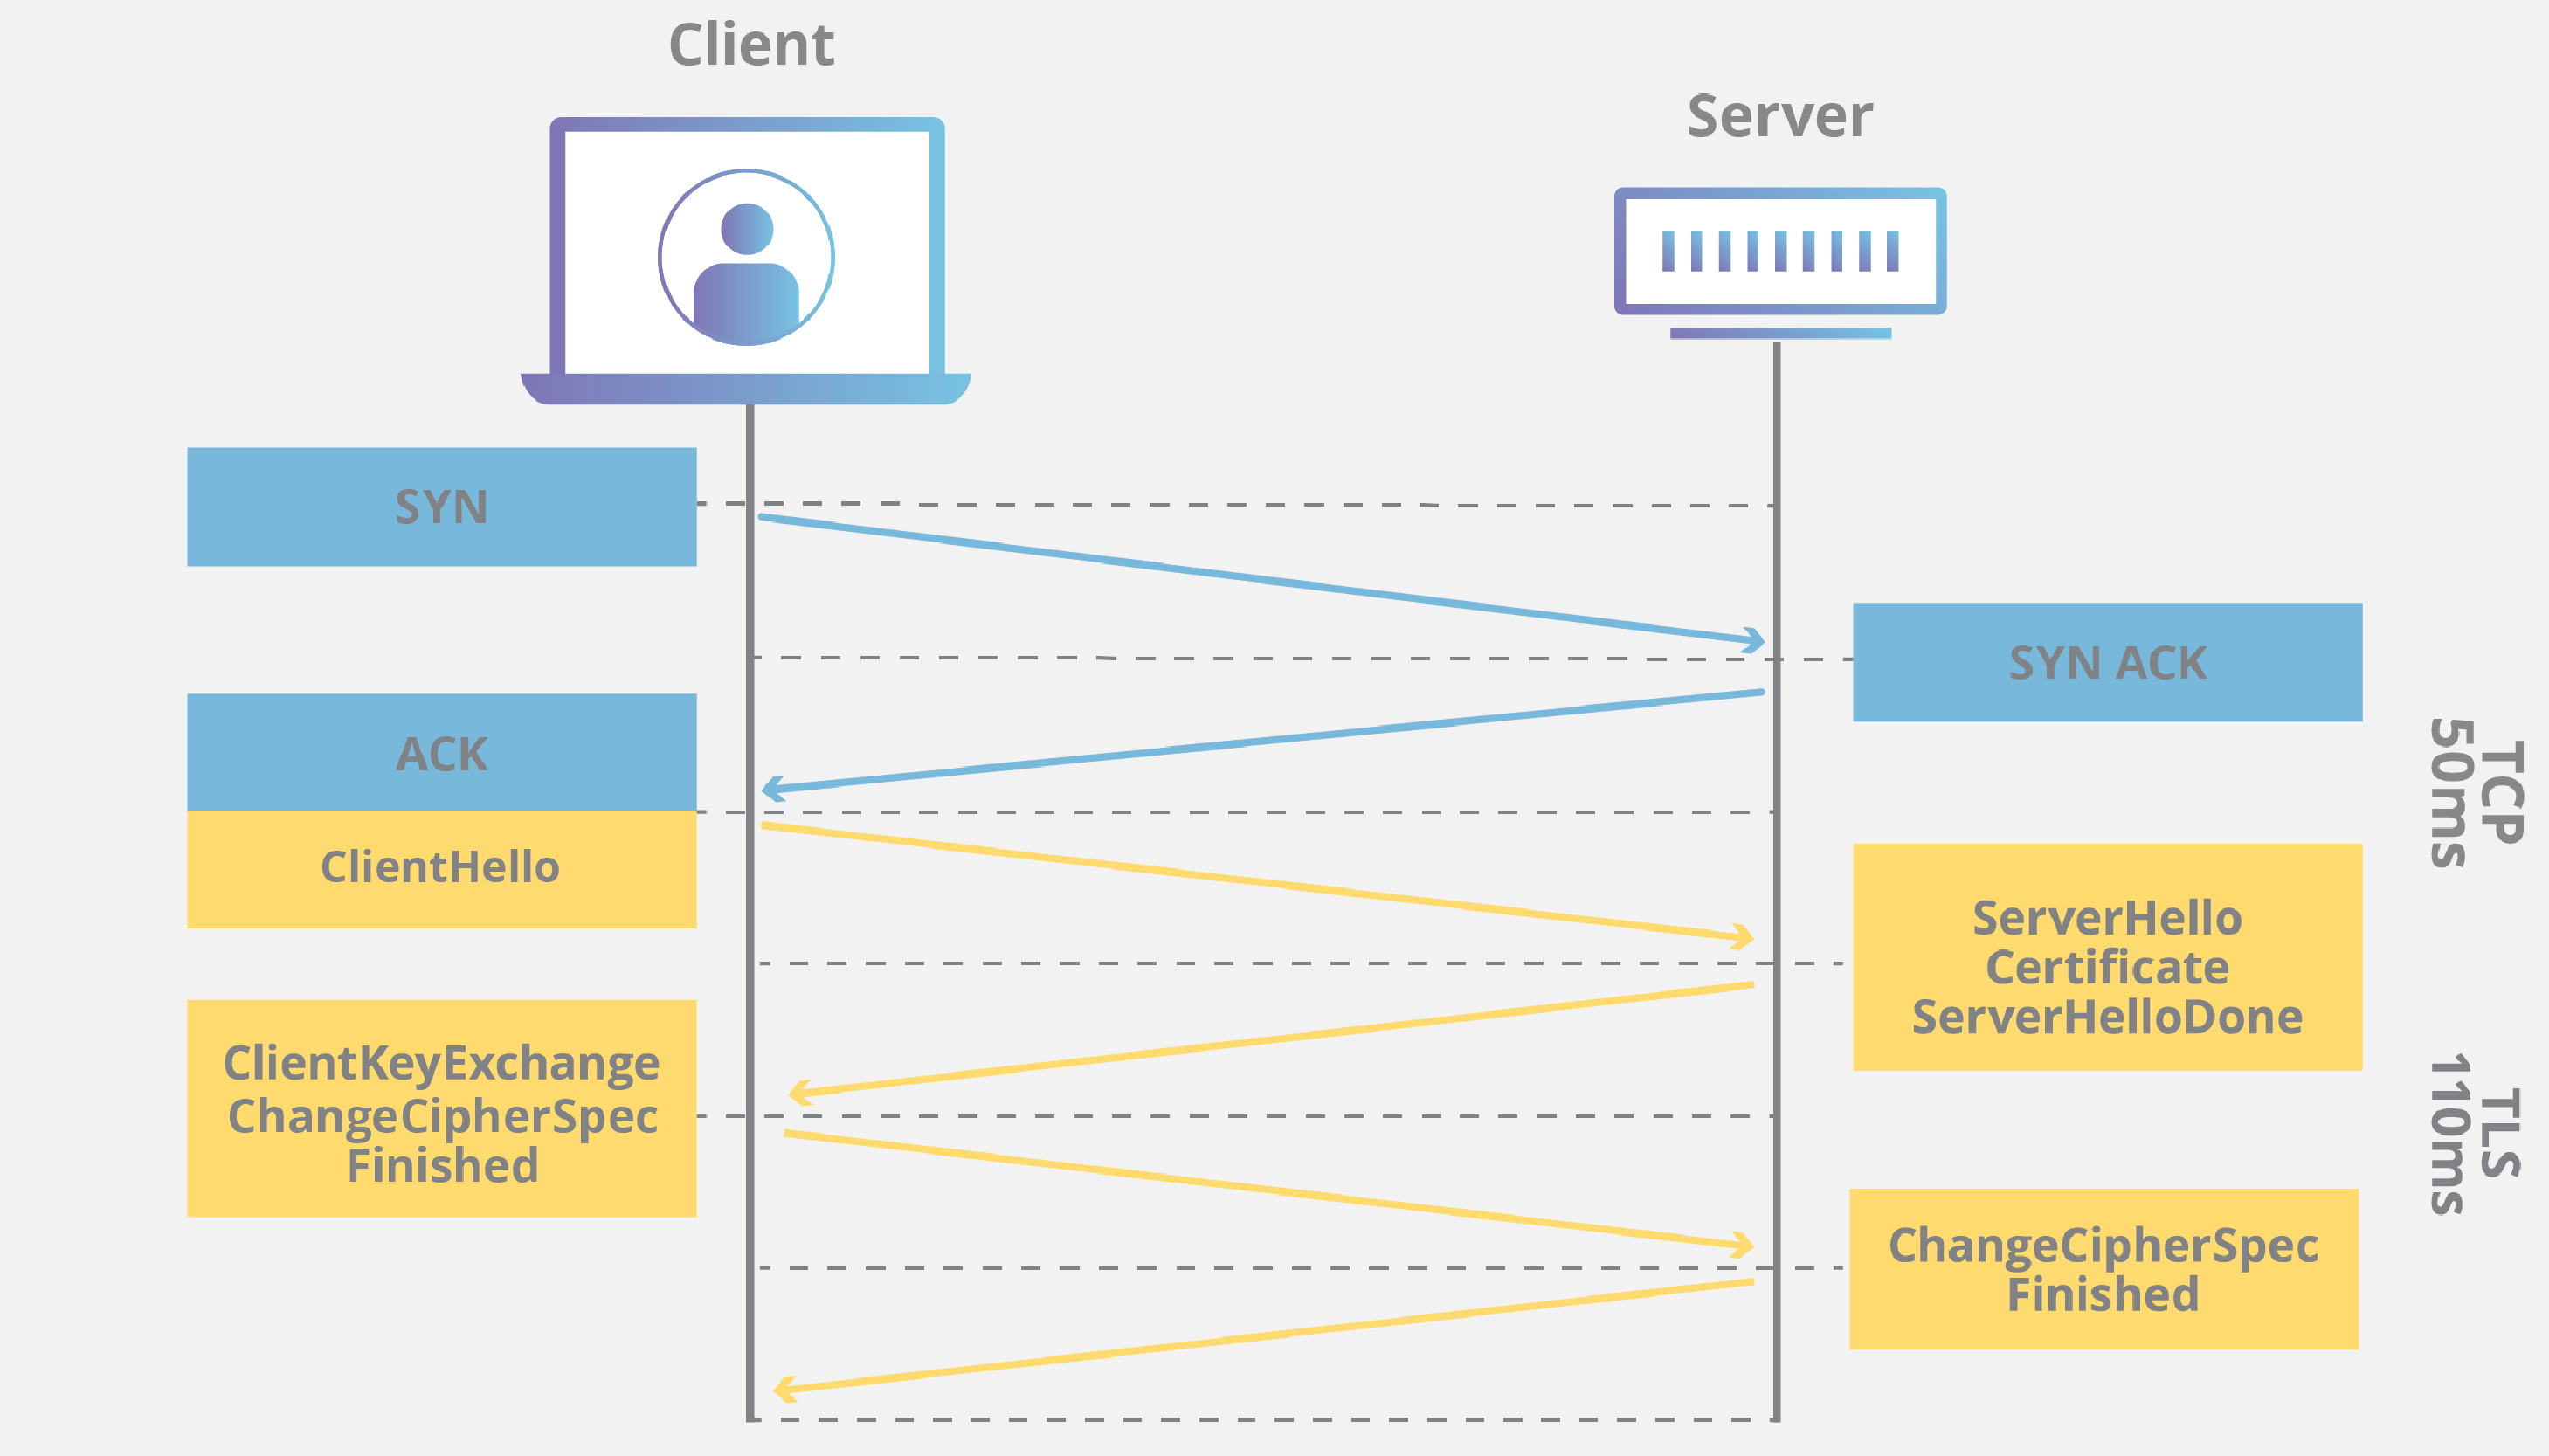
\includegraphics[width=14.5cm]{images/tls.png}
    \caption{Prikaz TCP i TLS rukovanja\citep{TLS}}
    \label{fig:tls}
\end{figure}

\subsubsection{CoAP}
CoAP \engl{Constrained Application Protocol}\citep{COAP} je specijalizirani protokol za uređaje ograničenih resursa te kao protokol transportnog sloja koristi UDP na vratima 5683. Protokol je dizajniran za pouzdani prijenos podataka u okolinama male propusnosti i visoke razine zagušenja prometa upotrebom malih zaglavlja paketa i potrebi za maloj procesnoj snazi za obradu zahtjeva. CoAP kao i HTTP djeluje na temelju zahtjeva i dogovora između klijenta i poslužitelja, a koristi URI shemu za identificiranje resursa na mrežnoj lokaciji. Metode koje se koriste u zahtjevima su identične HTTP-u te se temelje na REST \engl{Representational State Transfer} arhitekturi. Metode zahtjeva su definirane kodnim brojem u zaglavlju poruke koje definira i kodni broj statusa odgovora. Kodni broj je veličine 8 bitova. Podržane metode su prikazane u tablici.
\begin{table}[H]
    \centering
    \caption{Podržane metode CoAP zahtjeva}
    \begin{tabular}{| L | L | M |} 
    \hline
    \textbf{Metoda} & \textbf{Funkcionalnost} & \textbf{Svojstva}\\
    \hline\hline
    GET & dohvaća resurs na navedenom URI-u & sigurna, idempotentna \\
    \hline
    POST & stvara priloženi resurs na navedenom URI-u & nije sigurna ni idempotentna \\ 
    \hline
    PUT & ažurira ili stvara priloženi resurs na navedenom URI-u & nije sigurna, idempotentna \\ 
    \hline
    DELETE & briše resurs na navedenom URI-u & nije sigurna, idempotentna \\ 
    \hline
    \end{tabular}
    \label{tab:coap}
\end{table} 

CoAP podržava četiri vrste poruka:
\begin{description}
    \item[CON(Confirmable Message):]Svaka poruka treba dobiti odgovor ACK ili RESET kao potvrdu.
    \item[NON(Non-Confirmable Message):]Poruke ne trebaju dobiti potvrdu primitka.
    \item[ACK(Acknowledgement Message):]Potvrda da je specifična CON poruka zaprimljena.
    \item[RESET(Reset Message):]Potvrda da je specifična CON ili NON poruka zaprimljena, ali je kontekst poruke nedovoljan da bi se poruka obradila.
\end{description}

CoAP nudi mogućnost promatranja resursa temeljen na pretplati i objavi arhitekturi. Klijent registrira pretplatu na određeni resurs korištenjem zaglavlja opcija u kojem postavlja opciju \emph{Observe:0}. Nakon toga se svakim ažuriranjem resursa šalje poruka na pretplaćenog klijenta sve dok klijent ne otkaže pretplatu slanjem opcije \emph{Observe:1}. Na ovaj način se smanjuje broj potrebnih razmijenjenih poruka jer se izbjegava periodično slanje zahtjeva klijenta.

Kao što se HTTP osigurava upotrebom TLS-a preko TCP-a, tako CoAP koristi DTLS \engl{Datagram Transport Layer Security} za šifriranje i autentifikaciju. DTLS funkcionira na istom principu kao i TLS koji je objašnjen u HTTP odjeljku. CoAP s uključenim DTLS-om za razliku od HTTPS-a koristi UDP kao protokol transportnog sloja na vratima 5684.

\subsubsection{MQTT}
MQTT \engl{Message Queuing Telemetry Transport} je lagani protokol temeljen na porukama, koristi TCP kao protokol transportnog sloja na vratima 1883 te se bazira na topologiji PUSH/SUBSCRIBE. Arhitektura protokola MQTT sadrži dvije vrste sudionika: klijente i posrednike \engl{broker}.Posrednik je poslužitelj s kojim klijenti komuniciraju putem poruka te posrednik prosljeđuje te poruke na ostale klijente. Tako klijenti ne komuniciraju s ostalim klijentima već putem posrednika. Svaki klijent može biti izdavač \engl{publisher}, pretplatnik \engl{subscriber} ili oboje. 

MQTT je protokol temeljen na događajima te tako nema periodičnog ili stalnog prijenosa podataka čime se smanjuje količina prijenosa. Izdavač šalje poruke jedino kada ima informacije za slanje, a posrednik prosljeđuje poruke pretplatnicima kada primi nove informacije. Još jedan način smanjenja količine prijenosa podataka je korištenjem strogo definiranom, malom konstrukcijom poruka. Svaka poruka sadrži zaglavlje od samo dva bajta, ali može sadržavati i dodatno neobavezno zaglavlje, dok je sadržaj poruke ograničen na 256MB. 

Tri različite razine kvalitete usluge su dostupne kako bi se moglo odabrati između smanjenja količine i osiguravanja pouzdanosti prijenosa podataka. Nulta razina definira slanje poruka pretplatnicima bez potvrde je li poruka primljena, kod prve razine posrednik čeka potvrdu poruke te ako dođe do isteka vremena poruka se ponovno šalje te tako pretplatnik može poruku primiti više puta. Druga razina koristi četverostruko rukovanje između klijenta i posrednika kako bi se osiguralo da je poruka primljena i to točno jedan put. Za prvu i drugu razinu poruke se spremaju za klijente koji nisu trenutno dostupni te se ponovno šalju kada klijent postane ponovno dostupan. Na sljedećoj slici je prikazana topologija sudionika protokola MQTT.
\begin{figure}[htb]
    \centering
    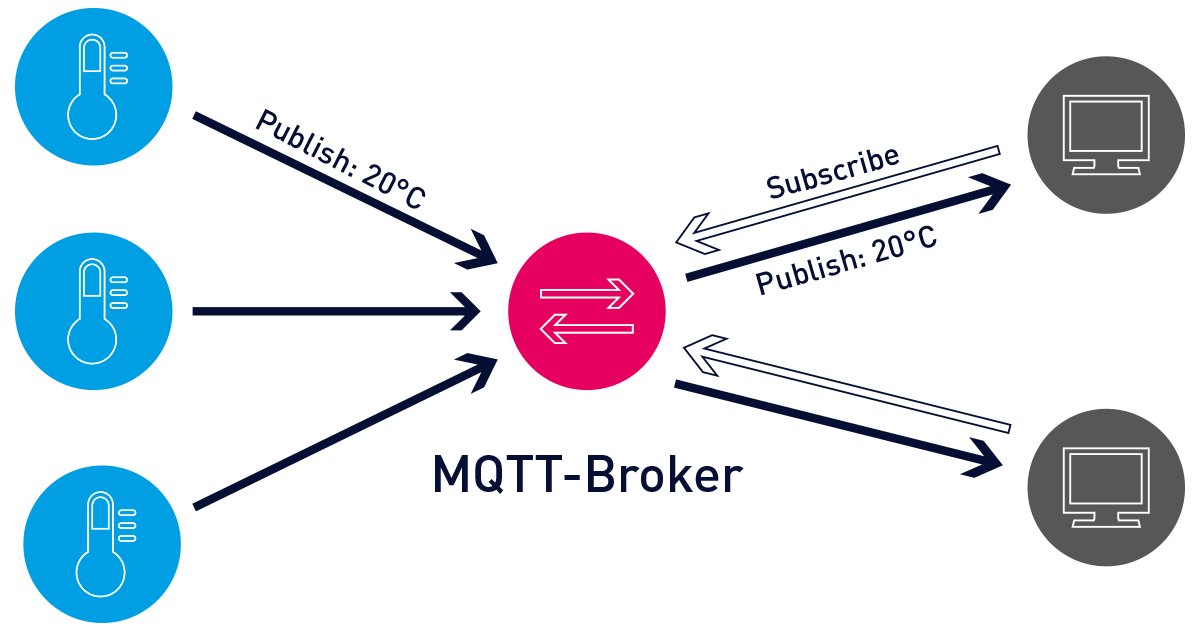
\includegraphics[width=11cm]{images/mqtt.png}
    \caption{Topologija sudionika protokola MQTT\citep{MQTT}}
    \label{fig:mqtt}
\end{figure}

Poruke koje izdavači objave se temelje na temama. Teme su strukturirane u hijerarhiju koja teme odvaja znakom "/" kao i kod datotečnih sustava. Primjer takve strukture je \textbf{"FER/zgrada-C/kat-7/soba-04/senzor/temperatura"} koja dozvoljava pretplatniku da navede kako želi primati samo informacije o temperaturi sobe četiri sedmog kata FER-ove C zgrade ili da se želi pretplatiti na sve senzore na FER-u koristeći sintaksu "FER/+/+/+/senzor/+". Kod objave prve poruke na temu koja ne postoji ta tema se automatski definira na posredniku bez prethodne konfiguracije.

MQTT podržava 14 vrsta poruka od kojih su osam potvrde, a šest zahtjevi opisani u nastavku.
\begin{description}
    \item[PUBLISH:]izdavač šalje podatke teme na posrednika. Ako tema ne postoji, ona se stvara na posredniku. Ovisno o definiranoj razini kvalitete usluge posrednik šalje potvrdu o primitku poruke.
    \item[SUBSCRIBE/UNSUBSCRIBE:]pretvara klijenta u pretplatnika na temu ili uklanja pretplatu na temu. Pretplate mogu biti vezane uz specifičnu temu, sve teme određene razine hijerarhije ili samo određene dijelove određenih razina hijerarhije tema. Kao odgovor klijent dobiva potvrdu od posrednika.
    \item[PING:] Klijent provjerava je li TCP konekcija prema posredniku još uvijek živa. Kao odgovor se dobiva potvrda ako je posrednik dostupan i TCP konekcija živa.
    \item[CONNECT/DISCONNECT:] Klijent šalje poruku posredniku za otvaranje ili zatvaranje konekcije. Kao odgovor se dobiva potvrda od posrednika o uspostavi konekcije, a kod zatvaranja konekcije se ne šalje potvrda.
\end{description}

Originalan cilj protokola MQTT je bilo smanjenje količine i efikasnost prijenosa podataka kako bi se mogla omogućiti komunikacija putem skupih i nepouzdanih komunikacijskih kanala poput satelitskog prijenosa. Tako kod razvoja protokola sigurnost nije bila primarna briga. Unatoč tome MQTT nudi nekoliko sigurnosnih mehanizama poput korištenje korisničkog imena i lozinke za autorizaciju klijenta kod posrednika. Nedostatak kod implementacije autorizacije je što se korisničko ime i lozinka prenose u nešifriranom tekstualnom formatu. Problem šifriranja i autentifikacije je riješeno korištenjem protokola TLS te se tada protokolu pristupa putem TCP vrata 8883. 

\subsection{Usporedba sigurnosnih mehanizama i primjena}
Sva tri navedena protokola nemaju vlastite mehanizme koji bi omogućavali šifriranje podataka i autentifikaciju te za to koriste protokol TLS kao nadogradnju. HTTP i MQTT koriste TLS s TCP-om kao protokol transportnog sloja dok CoAP koristi DTLS koji koristi UDP za protokol transportnog sloja. TLS i DTLS su funkcijski identični protokoli s jedinom razlikom u korištenom transportnog protokolu. HTTP i MQTT također imaju neobaveznu podršku za autorizacijom klijenta korištenjem korisničkog imena i lozinke.

HTTP je u svojoj primjeni puno fleksibilniji zbog mogućnosti prijenosa bilo koje vrste podataka koji uključuju hipertekstualne datoteke, slike, video i audio zapisa te kao takav je najzastupljeniji protokol aplikacijskog sloja na Internetu. Za razliku protokoli MQTT i CoAP su dizajnirani kao lagani protokoli za uređaje i mreže ograničenih resursa. Tako je glavna namjena tih protokola kod praćenja očitanja i jednostavnih događaja pretežito prisutnih u Internetu stvari.

\chapter{Sustav za praćenje tjelesne temperature}
Kako bi se olakšalo praćenje kretanja tjelesne temperature te smanjila potreba za ručnim mjerenjem korištenjem termometara, razvijen je sustav za praćenje tjelesne temperature. Cilj ovog sustava je omogućiti korištenje prijenosnog termometra koji se nalazi prilijepljen uz tijelo korisnika kako bi se mogao pratiti trend tjelesne temperature u razmaku minutnog intervala. Pregled podataka i upravljanje uređajima se odvija putem internet preglednika kako bi se s udaljenog mjesta mogao imati nadzor nad temperaturom korisnika.

\section{Korišteni razvojni alati i uređaji}
\subsection{Golang}
Golang\citep{Golang} je proceduralno i statičko pisani programski jezik sa sintaksom sličnom programskom jeziku C. Nudi bogati izbor standardnih biblioteka, dinamičko upravljanje memorijom i mogućnosti za visoku razinu konkurentnosti. Jezik je razvijen 2007. godine u Googleu te je 2009. objavljen kao jezik otvorenog koda, a zadnja verzija je 1.16.5 te je jedan od programskih jezika koji je u zadnjih nekoliko godina dosegao visoku razinu popularnosti. Golang se najaviše koristi kao HTTP poslužitelj i jedan je od jezika koji je popularizirao razvoj aplikacija temeljenih na mikroservisnoj arhitekturi.

\subsection{Fiber}
Fiber\citep{Fiber} je Golang razvojni okvir namijenjen za HTTP poslužitelje. Dizajniran je za jednostavan i brz razvoj HTTP poslužitelja s naglaskom na performansama i velikom broju konkurentnih korisnika. 

\subsection{React}
React\citep{React} je JavaScript biblioteka za razvoj korisničkih sučelja. Omogućuje jednostavan razvoj interaktivnih sučelja temeljenih na komponentama koje upravljaju vlastitim stanjima i na temelju promjena stanja reagiraju na promjene kako bi se ažurirali ili prikazali potrebni dijelovi sučelja.

\subsection{PostgreSQL}
PostgreSQL\citep{PostgreSQL} je objektno-relacijska baza podataka otvorenog koda. PostgreSQL je u razvoju više od 30 godina te ima reputaciju kao pouzdana, robusna baza podataka visokih performansi s velikim brojem značajki. 

\subsection{Docker}
Docker\citep{Docker} je platforma za kreiranje i pokretanje aplikacija na ponovljiv način korištenjem kontejnera. Kontejneri dozvoljavaju pakiranje aplikacija sa svim bibliotekama, ovisnostima i programskim kodom potrebnim da se aplikacija izvršava kao jedan paket, tj. slika. Kontejneri su lagani virtualni operativni sustavi koji umjesto korištenja cijelog operativnog sustava kao jedan paket iskorištavaju jezgru operativnog sustava domaćina te tako smanjuju veličinu slike potrebne za pokretanje.

\subsection{Nginx}
Nginx\citep{NGINX} je HTTP i zastupnički \engl{reverse proxy} poslužitelj, raspodjelitelj opterećenja i priručno spremište \engl{cache}. Nginx je programska podrška otvorenog koda te je jedan o najpopularnijih \emph{web} poslužitelja na Internetu gdje se najčešće koristi kao raspodjelitelj opterećenja.

\subsection{ESP32}
Joy-IT NodeMCU-ESP32\citep{ESP32Img} je varijanta ESP32 integriranog računala s mikrokontrolerom od proizvođača Joy-IT. ESP32 nudi dva komunikacijska modula za Wi-Fi 802.11 b/g/n i Bluetooth s podrškom za BLE. Priključni pinovi dozvoljavaju laku integraciju analognih senzora, a micro USB priključak omogućuje lako priključivanje vanjskih prijenosnih baterija za napajanje uređaja. ESP32 je energetski učinkovito računalo s podrškom za duboki san kako bi se uvelike smanjila potrošnja energije kada uređaj ne treba vršiti nikakvu funkciju.

\newpage
\section{Arhitektura i dizajn sustava}
Sustav za praćenje tjelesne temperature se sastoji od 4 glavne komponente: 
\begin{itemize}
    \item baze podataka,
    \item back-end aplikacije,
    \item front-end aplikacije,
    \item uređaja.
\end{itemize}
Baza podataka, back-end i front-end aplikacije se izvršavaju u zasebnim docker kontejnerima kako bi se olakšalo postavljanje u produkciju. Docker kontejneri dozvoljavaju da se sve komponente izvršavaju u jednakoj okolini neovisno o računalu na kojem se izvršavaju te se tako izbjegavaju nekompatibilnosti koje pojavljuju kada se program izvršava u različitim operacijskim sustavima. Pristup front-end i back-end aplikacijama se izvodi preko Nginx-a kao zastupničkog poslužitelja koji preusmjerava zahtjeve na određenu aplikaciju ovisno o URL-u te omogućuje uspostavljanje sigurne HTTPS veze između klijenta i aplikacija. Arhitektura sustava je prikazana na sljedećoj slici.
\begin{figure}[H]
    \centering
    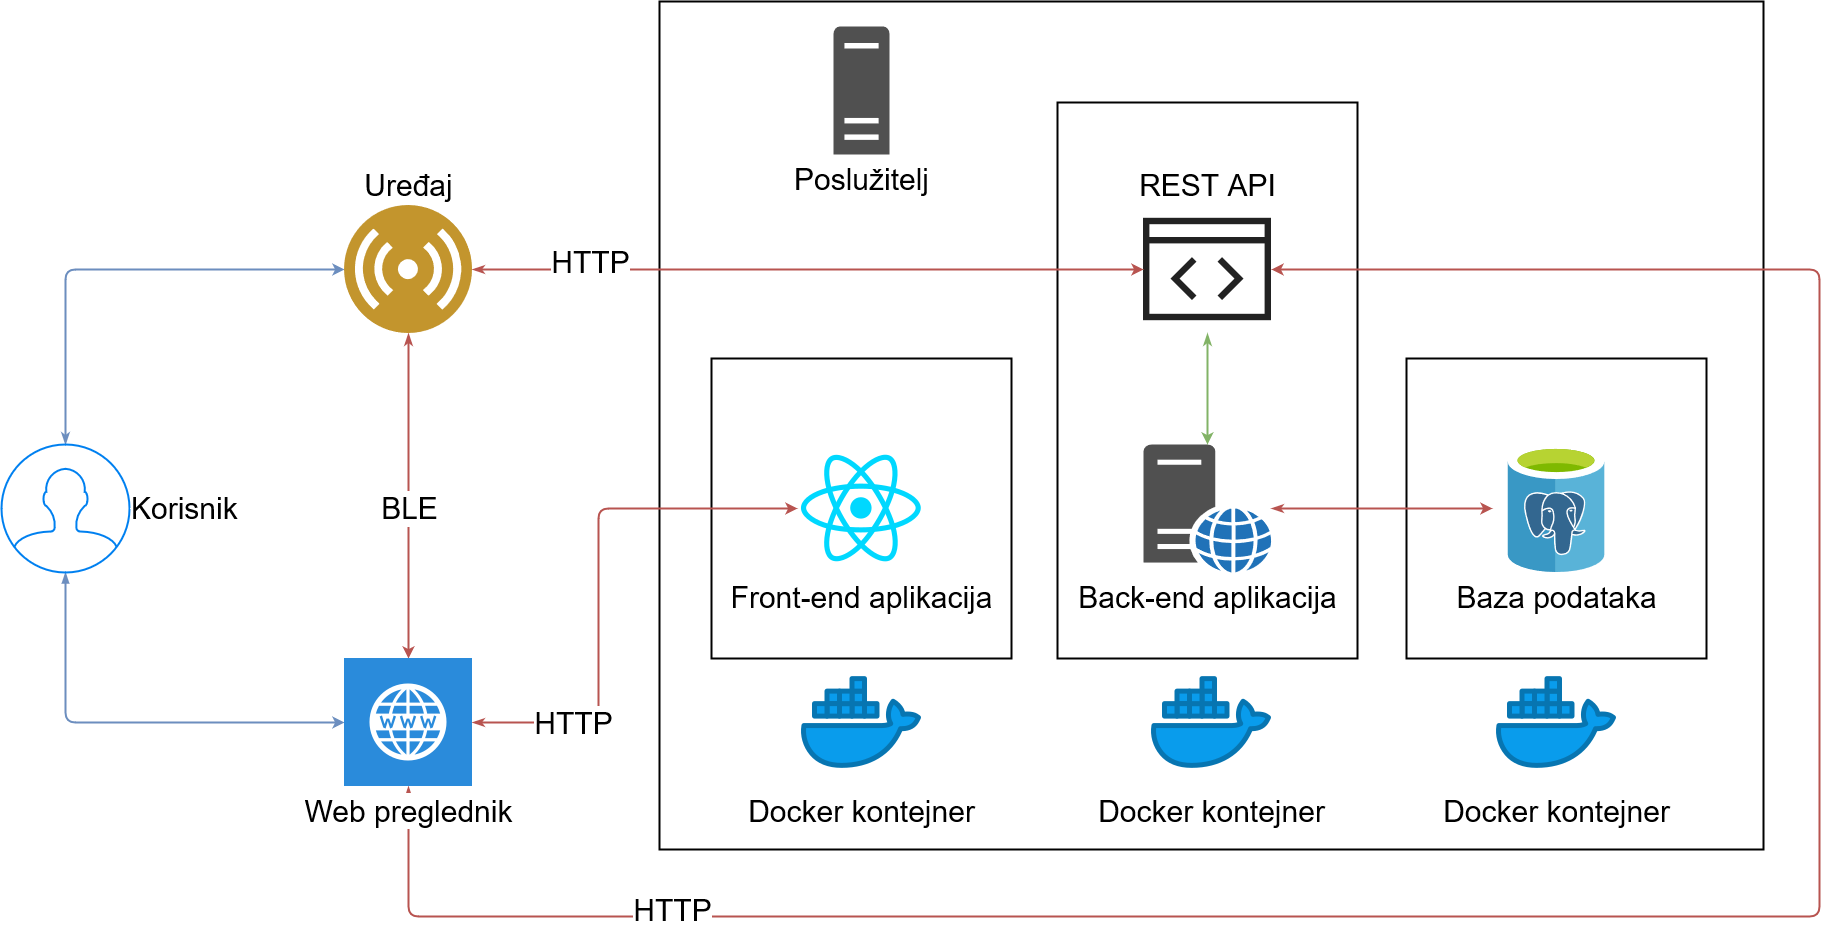
\includegraphics[width=14.5cm]{images/arh.png}
    \caption{Arhitektura sustava}
    \label{fig:architecture}
\end{figure}

Pristup svim funkcionalnostima sustava se izvodi preko internet preglednika putem kojeg se radi pregled informacija i upravljanje korisnicima te konfiguracija i upravljanje uređajima.

\subsection{Baza podataka}
Podaci sustava se spremaju u PostgreSQL bazu podataka koja se izvršava u Docker kontejneru. Baza se sastoji od 4 tablice te je relacijska shema baze prikazana na sljedećoj slici.
\begin{figure}[H]
    \centering
    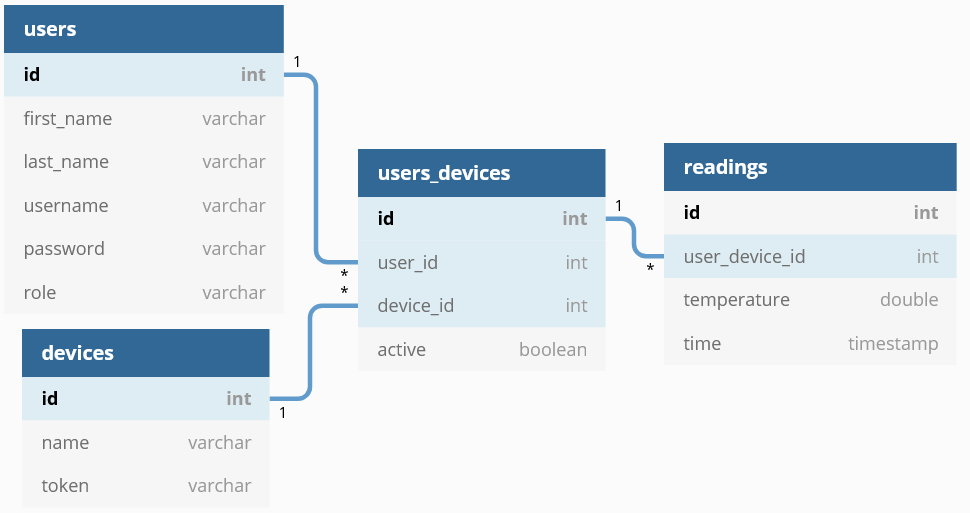
\includegraphics[width=14.5cm]{images/baza.png}
    \caption{Baza podataka}
    \label{fig:baza}
\end{figure}

Tablica \emph{users} predstavlja korisnike sustava te ovisno o ulozi \engl{role} definira administratore i korisnike za koje se promatra temperatura. Tablica \emph{devices} predstavlja uređaje koji se koriste za opažanje temperature te je definirano ime i pristupni \emph{token} uređaja. Tablica \emph{users\_devices} predstavlja vezu između korisnika i uređaja kod koje stupac \emph{active} određuje za koji uređaj je trenutno pridijeljen korisnik. Jedan uređaj ima pridijeljenog jednog korisnika te je tada stupac \emph{active} istinit. Tablica \emph{readings} predstavlja očitanja koja uređaj opaža te su definirani stupci koji predstavljaju temperaturu i vrijeme kada je temperatura očitana. Definicija tablica i relacijskih veza se nalazi u datoteci: \path{implementation/database/db.sql}

\subsection{Back-end aplikacija}
Back-end aplikacija je pisana u Golang programskom jeziku te se koristi Fiber razvojni okvir za razvoj HTTP poslužitelja. Aplikacija se izvršava u Docker kontejneru te se zahtjevi na poslužitelj preusmjeravaju s Nginx-a. Zahtjevi na aplikaciju dolaze s dva izvora: front-end aplikacije koja se izvršava u internet pregledniku i uređaja. Aplikacija je dizajnirana po REST arhitekturi gdje se pristup određenim resursima odvija na temelju URL-a definiranog u zahtjevu. Aplikacija obrađuje zahtjeve te komunicira s bazom podataka kako bi dohvatila ili spremila potrebne podatke. Programska podrška aplikacije se sastoji od sljedećih datoteka koje se nalaze na putanji: \path{implementation/backend/}

\begin{description}
    \item[go.mod:] definira verziju Golanga i sve vanjske biblioteke potrebne za izvršavanje i prevođenje programske potpore.
    \item[go.sum:] definira URL, verzije i identifikacijske oznake biblioteka koje su potrebne za izvršavanje i prevođenje programske potpore.
    \item[main.go:] predstavlja prvobitni dio aplikacije u kojem se inicijaliziraju svi potrebni dijelovi poput konekcija s bazom podataka, HTTP poslužitelj, rute koje obrađuju određene funkcije na temelju REST arhitekture i posrednička funkcija za autorizaciju korisnika. 
    \item[routes.go:] definira rute i funkcije koje obrađuju zahtjeve na određenom URL-u.
    \item[auth.go:] Definira funkcije za logiranje i registraciju korisnika te posredničku funkciju za autentifikaciju i autorizaciju korisnika kada pristupa određenim resursima sustava.
    \item[handlers.go:] definira sve funkcije REST arhitekture koje obrađuju zahtjeve za određenim resursima sustava.
    \item[models.go:] definira strukture tablica baze podataka i svih zahtjeva i odgovora.
\end{description}

\subsection{Front-end aplikacija}
Front-end aplikacija je pisana u JavaScript razvojnom okviru React. Sama aplikacija se izvršava u internet pregledniku dok se u zasebnom docker kontejneru na poslužitelju odvija dohvat potrebnih datoteka. Datoteke aplikacije se nalaze na putanji: \path{implementation/frontend/}. U \emph{package.json} datoteci se nalaze definirane biblioteke koje aplikacija koristi, podržani internet poslužitelji i skripte za izvršavanje. U \path{src} mapi se nalazi sva potrebna programska podrška koja se izvršava u internet pregledniku. Neke od datoteka i mapa u \path{src} folderu su opisane u nastavku.
\begin{description}
    \item[index.js:] pristupna datoteka aplikacije koja enkapsulira ostatak aplikacije.
    \item[index.css:] definira CSS stilove za osnovne HTML klase.
    \item[App.js:] glavni dio aplikacije koji definira usmjeritelj na ostale komponente ovisno o URL-u i o tome je li korisnik prijavljen.
    \item[App.css:] definira CSS stilove za HTML klase komponenata.
    \item[components/*:] ova mapa definira komponente koje se koriste u aplikaciji poput komponenti za prijavu, registraciju, navigacijsku traku, konfiguraciju uređaja i prikaz grafa i tablice očitane temperature.
\end{description}

Aplikacija komunicira s back-end aplikacijom putem protokola HTTP kako bi dohvatila potrebne podatke te je potrebno prvobitno biti prijavljen kako bi se dohvaćanje podataka moglo odvijati. Za potrebe konfiguracije uređaja koristi se komunikacija protokolom BLE. Konfiguracija uređaja se može odvijati samo putem internet preglednika koji podržavaju protokol BLE i koji se izvršavaju na računalu s kompatibilnim Bluetooth komunikacijskim modulom.

\subsection{Uređaj za mjerenje temperature}
Za potrebe mjerenja temperature se koristi Joy-IT NodeMCU-ESP32 integrirano računalo s Velleman VMA320 analognim senzorom za toplinu. Napajanje uređaja se vrši putem vanjske prijenosne baterije koja je priključena na micro USB priključak. Analogni senzor je povezan s uređajem putem 3 priključnih pinova za ulaz, napajanje i uzemljenje. Shema spajanja uređaja sa senzorom i baterijom je prikazana na sljedećoj slici.
\begin{figure}[H]
    \centering
    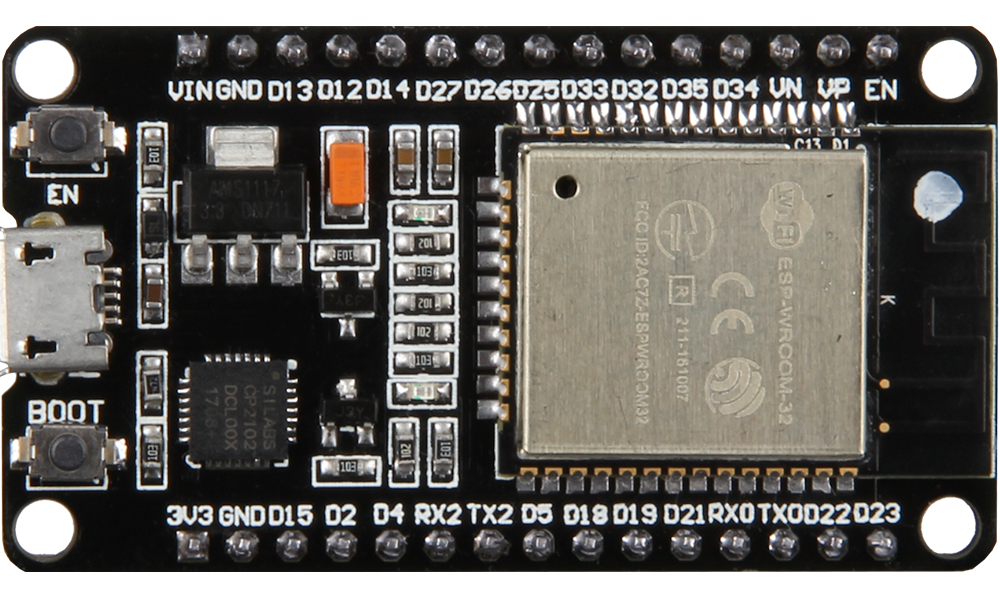
\includegraphics[width=6.5cm, angle=90]{images/esp32.png}
    \caption{Shema spajanja}
    \label{fig:device}
\end{figure}

Uređaj komunicira putem dva komunikacijska protokola. Putem protokola Wi-Fi komunicira s internet poslužiteljem na kojem se izvršava back-end aplikacija kako bi poslao očitanja temperature. Putem protokola BLE komunicira s internet preglednikom na kojem se izvršava front-end aplikacija za potrebe konfiguracije uređaja. Kako bi uređaj mogao komunicirati s back-end aplikacijom potrebno je konfigurirati parametre opisane u nastavku.
\begin{description}
    \item[ID:] identifikator uređaja.
    \item[Token:] pristupni token kojim se autentificira uređaj.
    \item[Host:] domena internet poslužitelja na kojem se izvršava back-end aplikacija.
    \item[SSID:] identifikator pristupne Wi-Fi točke.
    \item[Password:] lozinka za pristupnu Wi-Fi točku.
\end{description}

Programska podrška uređaja se nalazi u datoteci: \path{implementation/esp32/module.ino}


\section{Opis rada sustava}
Sustav za praćenje tjelesne temperature sadrži sedam glavnih obrazaca uporabe koji su opisani u nastavku.

\subsection{Registracija korisnika}
Kako bi korisnik dobio pristup sustavu potrebno je da se prvo registrira. Registraciji je moguće pristupiti ako korisnik nije već prijavljen na sustav. Registracija se provodi upisivanjem željenog korisničkog imena, imena i prezimena korisnika te željene lozinke. Kada korisnik ispuni podatke obrasca i pritisne gumb \emph{Registriraj} podaci se šalju na back-end aplikaciju gdje se spremaju u bazu podataka.

\subsection{Prijava korisnika}
Nakon registracije korisnika potrebno je da se korisnik prijavi kako bi mogao pristupiti sustavu. Prijava se vrši ispunjavanjem obrasca u koji je potrebno unijeti korisničko ime i lozinku. Nakon pritiska na gumb \emph{Prijavi} podaci obrasca se šalju na back-end aplikaciju gdje se odrađuje autorizacija korisnika na temelju podataka iz baze. Ako su podaci točni korisnik se uspješno prijavio na sustav te ga se preusmjerava na dio sustava koji je dostupan samo prijavljenim korisnicima. 

\subsection{Kreiranje korisnika}
Kreiranje korisnika se odvija unošenjem podataka o imenu i prezimenu korisnika. Tako se kreira korisnik uloge \emph{Pacijent} koji nema pristup sustavu nego mu se samo može dodjeliti uređaj i pratiti podaci o njegovoj temperaturi.

\subsection{Uređivanje korisnika}
Uređivanje korisnika se odvija promjenom podataka i dodjeljivanjem uređaja koji će daljnje biti povezan s tim korisnikom.

\subsection{Konfiguracija uređaja}
Konfiguracija uređaja se odvija prvo povezivanjem putem protokola BLE s uređajem. Kako bi se mogao konfigurirati uređaj potrebno je unijeti pristupnu lozinku za uređaj. U obrazac se upisuju pristupni token, domena poslužitelja, SSID i lozinka Wi-Fi pristupne točke koje se zatim šalju na uređaj s identifikatorom uređaja. Osim na uređaj ti podaci se šalju i na back-end aplikaciju. Konfiguracijom uređaja počinje očitavanje tjelesne temperature.

\subsection{Očitavanje tjelesne temperature}
Uređaj svake minute očitava temperaturu sa senzora te šalje zahtjev s podacima o identifikatoru uređaja, očitanoj temperaturi i pristupnom tokenu na back-end aplikaciju. Aplikacija provjerava token i identifikator u bazi podataka i ako podaci zahtjeva odgovaraju podacima u bazi, aplikacija sprema podatke o izmjerenoj temperaturi i vrijeme mjerenja u bazu.

\subsection{Pregled trenda kretanja temperature}
Prijavljeni korisnik može pregledavati trend kretanja temperature za korisnike koji postoje u sustavu. Kod pregleda se prikazuje linijski graf gdje x-os predstavlja vrijeme, a y-os temperaturu. uz graf se prikazuje i tablica s vremenom i temperaturnim očitanjima.

\section{Sigurnosna analiza sustava}
Analiza sustava će se provoditi kroz zahtjeve vezane uz sigurnost i privatnost koji su definirani u odjeljku 3.1.

\subsection{Tajnost}
Tajnost podataka je očuvana korištenjem autentifikacije i autorizacije korisnika na sustavu. To se provodi prijavom korisnika na sustav kako bi mogao imati uvid u podatke o ostalim korisnicima i temperaturnim očitanjima. Kako bi se očuvala tajnost podataka u prijenosu koristi se protokol HTTP/S za komunikaciju između internet preglednika i poslužitelja te uređaja i poslužitelja. Komunikacija između internet preglednika i uređaja je također šifrirana korištenjem BLE sigurnosnih mehanizama, a postupak uparivanja se provodi \emph{Passkey} metodom kod koje je potrebno unijeti pristupnu lozinku koja je definirana na uređaju.

\subsection{Cjelovitost}
Cjelovitost informacija se omogućava korištenjem protokola HTTP/S koji uporabom transportnog protokola TCP omogućuje komunikaciju bez gubitka informacija, a korištenjem kriptografskog protokola TLS se osigurava točnost podataka.

\subsection{Raspoloživost}
Raspoloživost cijelog sustava ovisi o dostupnosti poslužitelja na kojem se izvršava cijeli sustav. Ako dođe do prekida rada poslužitelja tada nije moguće pristupiti podacima i spremati podatke o očitanjima. Veći stupanj raspoloživosti se može ostvariti korištenjem dodatne redundancije poslužitelja.

\subsection{Vjerodostojnost}
Vjerodostojnost poslužitelja se postiže korištenjem certifikata pomoću kojeg se autentificira poslužitelj. Vjerodostojnost uređaja se utvrđuje pomoću pristupnog tokena koji se nalazi u zahtjevu, a dodijeljen mu je od sustava. Vjerodostojnost korisnika se utvrđuje korištenjem pristupnog korisničkog imena i lozinke.

\subsection{Neporicanje}
Neporicanje se postiže bilježenjem izvršenih aktivnosti u sustavu. Bilježi se vrijeme, korisnik i podaci kojima je korisnik pristupao. Tako se naknadno mogu utvrditi aktivnosti korisnika.

\subsection{Odgovornost}
Odgovornost u sustavu se postiže istim mehanizmom bilježenja kao i neporicanje. Tako se postiže odgovornost korisnika o provođenim aktivnostima.

\subsection{Pouzdanost}
Konzistentno ponašanje sustava se postiže uporabom REST arhitekture za dohvat podataka koja omogućava korištenje jednostavnih funkcija za obradu svih zahtjeva. Pouzdanost kod uređaja se postiže jednostavnom logikom koja obavlja očitavanja, povezivanje i prijenos informacija na poslužitelj.

\chapter{Zaključak}
Razvoj pristupnih mreža i energetski učinkoviti uređaji malih dimenzija omogućili su pojavu Interneta stvari u našoj svakodnevici. Pametni uređaji su sve više dio naših života te nam nude uvid u informacije i automatizaciju različitih procesa s kojima se svakodnevno susrećemo. 

Dostupnost informacija o razvojnim alatima i niska cijena uređaja omogućuju jednostavan i brz razvoj pametnih uređaja i sustava Interneta stvari čime se proširuje broj različitih primjena. Tako se međuostalom dobiva konkurentnost na tržištu i veća integracija pametnih uređaja u živote korisnika.

Razvoj Interneta stvari donosi i mnoge izazove koji su vezani uz prirodu takvih sustava među kojima su raspodijeljenost, heterogenost, integracija, sigurnost i privatnost. Svi ti izazovi su međusobno povezani te je kod planiranja i razvoja sustava potrebno obratiti pažnju na njih, što se nekada očituje u zanemarivanju nekih od tih izazova.

Sigurnost i privatnost korisnika su izazovi s kojima se proizvođači najčešće susreću. Brz razvoj rješenja Internet stvari kako bi se proizvod prvi stavio na tržište uzrokuje razne sigurnosne propuste u sustavima čime se izravno ugrožava sigurnost i privatnost korisnika. Nedovoljna informiranost razvijatelja oko sigurnosnih praksi uz brz razvoj također utječe na krajnju sigurnost sustava.

Sigurnosni propusti ne utječu samo na privatnost korisnika već i na sigurnost šire zajednice. Napadi na sustave Interneta stvari omogućuju onesposobljavanje raznih industrijskih postrojenja čiji sigurnosni mehanizmi sprječavaju nastanak ekoloških katastrofa.

Kako bi se osigurala sigurnost sustava i privatnost podataka potrebna je dostupnost informacija vezanih uz uređaje i servise Interneta stvari. Dostupnošću informacija poput otvorenih i dostupnih implementacijskih detalja dozvoljava široj razvojnoj zajednici istraživanje i konačno obznanjenje otkrivenih propusta u sustavima. Informiranjem javnosti omogućuje se korisnicima da donesu informiranu odluku o proizvodima koje koriste i tako zaštite sebe i svoju okolinu.  

\bibliographystyle{fer}
\bibliography{literatura}
\listoffigures
\listoftables

\begin{sazetak}
Internet stvari je sve rašireniji u svakodnevici ljudi u kojoj pametni uređaji dozvoljavaju automatizaciju i kreiranje novih procesa. Stoga je sustave Interneta stvari potrebno osigurati dostupnim sigurnosnim mehanizmima. Kroz rad se obrađuju definicija, referentni model koji opisuje slojeve sustava, područja primjene i trendovi Interneta stvari. Definiraju se zahtjevi vezani uz sigurnost i privatnost sustava i korisnika te najčešći sigurnosni propusti u takvim sustavima. Provodi se analiza i komparacija sigurnosnih mehanizama određenih uređaja i protokola složaja Interneta stvari. Opisuje se implementacija sustava za praćenje kretanja tjelesne temperature, njegova arhitektura, dijelovi sustava te se provodi sigurnosna analiza cijelog sustava.  

\kljucnerijeci{Internet stvari, Informacijska sigurnost, ESP32, Wi-Fi, Bluetooth Low Energy, LoRaWAN, IP, TCP, UDP, HTTP, TLS, CoAP, MQTT, Analiza, Usporedba}
\end{sazetak}

\newpage
\engtitle{Analysis and comparison of IoT security mechanisms}
\begin{abstract}
The Internet of Things is becoming more widespread in people's everyday lives, where smart devices allow automation and the creation of new processes. Therefore, IoT systems need to be secured with available security mechanisms. The paper deals with the definition, the reference model that describes the layers of the system, areas of application and trends of the Internet of Things. The requirements related to the security and privacy of systems and users and the most common security failures in such systems are defined. The analysis and comparison of security mechanisms of certain devices and protocols of the Internet of Things protocol stack is performed. The implementation of the system for monitoring the change of body temperature, its architecture, parts of the system is described, and a safety analysis of the entire system is performed.

\keywords{Internet of Things, Information security, ESP32, Wi-Fi, Bluetooth Low Energy, LoRaWAN, IP, TCP, UDP, HTTP, TLS, CoAP, MQTT, Analysis, Comparison}
\end{abstract}

\end{document}